% ==== BEGIN OF PREAMBLE =======================================================
% ---- document class (use appropriate driver for DIV to PS/PDF conversion):
\documentclass[12pt,a4paper]{book}

% ---- my packages
\usepackage{datetime}
\newdateformat{monthyeardate}{\monthname[\THEMONTH] \THEYEAR}
\usepackage{listings}  % pretty print code lines
% Default fixed font does not support bold face
\DeclareFixedFont{\ttb}{T1}{txtt}{bx}{n}{12} % for bold
\DeclareFixedFont{\ttm}{T1}{txtt}{m}{n}{12}  % for normal
\lstset{language=Python, basicstyle=\ttm}
\usepackage{amsmath}  % standard math package
\usepackage{mathtools}
\usepackage{siunitx}  % display numbers and units
\sisetup{per-mode = reciprocal}
\DeclareSIUnit\year{yr}

% ---- graphicx package:
\usepackage{graphicx}


% ---- natbib package:
\usepackage{natbib}
\bibpunct{(}{)}{;}{a}{}{,}  % adjust author-year citation format 


% ---- hyperref package for cross-references:
\usepackage{hyperref}
% -- USE BLACK LINKS IN PRINTOUT (uncomment the following lines if necessary):
%\hypersetup{colorlinks,%
%            linktocpage,%
%            breaklinks,%
%            citecolor=black,%
%            filecolor=black,%
%            linkcolor=black,%
%            urlcolor=black,}
% -- use color links in pdf version (comment the following lines if necessary):
\hypersetup{colorlinks,
            linktocpage,%  make page number, not text, be link on TOC, LOF & LOT
            breaklinks,%
            citecolor=blue,%
            filecolor=blue,%
            linkcolor=blue,%
            urlcolor=blue,}


% ---- caption package:
\usepackage[font=small,labelfont=bf]{caption}


% ---- subfigure package:
\usepackage[tight,nooneline,FIGTOPCAP,bf]{subfigure}
% \setlength{\subfigcaptopadj}{-6pt}  % vertical position of subfigure labels
\renewcommand{\thesubfigure}{\alph{subfigure}}
\makeatletter
    \renewcommand{\@thesubfigure}{(\thesubfigure)}  % subfigure labels:     (a)
    \renewcommand{\@@thesubfigure}{\thesubfigure}   % produced by \subref:   a
    \renewcommand{\p@subfigure}{\thefigure}         % produced by \ref:   3.1a
\makeatother


% ---- fancyhdr package:
\usepackage{fancyhdr}


% ---- some other useful packages:
% \usepackage{showkeys}  % show all keys (labels)
% \usepackage{times}     % use times new roman instead of computer modern font


% ---- page layout:
\setlength{\textheight}{24cm}
\setlength{\textwidth}{15cm}
\setlength{\topmargin}{-0.9cm}
\setlength{\headheight}{0.6cm}
\setlength{\headsep}{1cm}
\setlength{\footskip}{1cm}
\setlength{\oddsidemargin}{9.1mm}
\setlength{\evensidemargin}{-0.2mm}
\setlength{\marginparwidth}{2cm}


% ---- paragraph and line properties:
\setlength{\parindent}{0.8cm}
\setlength{\parskip}{0pt}
\linespread{1.2}
\sloppy % reduce number of word divisions and use more space between words


% ---- header format: use fancyhdr page style:
\pagestyle{fancy}
\fancyhf{}
\renewcommand{\chaptermark}[1]{\markboth{#1}{}}
\renewcommand{\sectionmark}[1]{\markright{\thesection\ #1}}
\fancyhead[LE,RO]{\thepage}
\fancyhead[LO]{\slshape \small \rightmark}
\fancyhead[RE]{\slshape \small \leftmark}
\renewcommand{\headrulewidth}{0pt}


% ---- define label format for equations, figures, and tables:
\renewcommand{\theequation}{\thechapter.\arabic{equation}}
\renewcommand{\thefigure}{\thechapter.\arabic{figure}}
\renewcommand{\thetable}{\thechapter.\arabic{table}}


% ==== END OF PREAMBLE =========================================================


% ==== BEGIN OF BODY ===========================================================
\begin{document}

% ---- my commands
\newcommand{\vas}{volume/area scaling}
\newcommand{\Vas}{Volume/area scaling}
\newcommand{\tstar}{$t^*$}
\newcommand{\mustar}{$\mu^*$}
\newcommand{\bias}{$\beta^*$}


% ==== START FRONT MATTER (use ROMAN numerals) =================================
\frontmatter


% ==== TITLE PAGE ==============================================================
% ---- include tex-file (CHOOSE APPROPRIATE FILE):
%!TEX root = thesis.tex
\begin{titlepage}
\begin{center}

% ---- main title
~\\[15mm]
{\Huge  {\bf Testing the importance of explicit glacier dynamics for
future glacier evolution in the Alps}}\\[5mm]


% ---- subtitle (if necessary):
% {\LARGE {\bf Subtitle}\\[15mm]


% ---- type of thesis:
{\Large \textsc{Master's Thesis}} \\[15mm]


% ---- field of study:
{\large in Atmospheric Sciences} \\[15mm]


% ---- institution:
{\large Submitted to the} \\[2mm]
{\Large \textsc{Department of Atmospheric and Cryospheric Sciences}} \\[2mm]
{\large of the} \\[2mm]
{\Large \textsc{University of Innsbruck}} \\[15mm]


% ---- degree:
{\large in Partial Fulfillment of the Requirements for the Degree of} \\[2mm]
{\Large \textsc{Master of Science}} \\[15mm]


% ---- author:
{\large by} \\[2mm]
{\Large \textsc{Moritz Oberrauch}} \\[15mm]


% ---- advisor:
{\large Advisor} \\[2mm]
{\large Fabien Maussion, PhD} \\[15mm]


% ---- location, date:
{\large Innsbruck, \monthyeardate{\today}}


\end{center}
\end{titlepage}

\newpage
~\thispagestyle{empty}
\newpage
% ---- start page numbering again:
\setcounter{page}{1}


% ==== DEDICATION ==============================================================
% ---- include tex-file:
%!TEX root = thesis.tex
% \addcontentsline{toc}{chapter}{Dedication}
\thispagestyle{plain}

\begin{flushright}
 \Large\em\null\vskip5cm To Psycho \\
 \large And all others who try to move their toes individually
\end{flushright}

\newpage
\thispagestyle{plain}


% ==== PREFACE =================================================================
% ---- include tex-file:
% %!TEX root = thesis.tex
\chapter*{Preface}
\addcontentsline{toc}{chapter}{Preface}
\thispagestyle{plain}

If I need a preface, I'll come back here later...

\begin{flushright}
\textit{Moritz Oberrauch}

\textit{Innsbruck, \monthyeardate{\today}} 
\end{flushright}

% \newpage
% \thispagestyle{plain}


% ==== ABSTRACT ================================================================
% ---- set some counters to zero:
\setcounter{equation}{0}
\setcounter{table}{0}
\setcounter{figure}{0}
% ---- include tex-file:
%!TEX root = thesis.tex
\chapter*{Abstract}
\addcontentsline{toc}{chapter}{Abstract}
\thispagestyle{plain}

% The abstract is a short summary of the thesis. It announces in
% a brief and concise way the scientific goals, methods, and most important
% results. The chapter ``conclusions'' is not equivalent to the abstract!
% Nevertheless, the abstract may contain concluding remarks. The abstract
% should not be discursive. Hence, it cannot summarize all aspects of the thesis
% in very detail. Nothing should appear in an abstract that is not also
% covered in the body of the thesis itself. Hence, the abstract should be the
% last part of the thesis to be compiled by the author.

% A good abstract has the following properties: \emph{Comprehensive:} All major
% parts of the main text must also appear in the abstract. \emph{Precise:}
% Results, interpretations, and opinions must not differ from the ones in the main
% text. Avoid even subtle shifts in emphasis. \emph{Objective:} It may contain
% evaluative components, but it must not seem judgemental, even if the thesis
% topic raises controversial issues. \emph{Concise:} It should only contain the
% most important results. It should not exceed 300--500 words or about one page.
% \emph{Intelligible:} It should only contain widely-used terms. It should
% not contain equations and citations. Try to avoid symbols and acronyms (or at
% least explain them). \emph{Informative:} The reader should be able to quickly
% evaluate, whether or not the thesis is relevant for his/her work.

% An Example: The objective was to determine whether \dots (\emph{question/goal}).
% For this purpose, \dots was \dots (\emph{methodology}). It was found that \dots
% (\emph{results}). The results demonstrate that \dots (\emph{answer}).

Global glacier models are imperative to project future glacier ice mass loss and the accompanied sea level rise. Glaciers are controlled by their mass balance and the resulting ice flow.
The scarcity of ice volume observations makes the calibration, and especially validation, of geometry models difficult. As a consequence, most global model use \vas{} relations instead of a dedicated ice physic model. Over the last years, the increasing accuracy and coverage of global data inventories, in combination with new and automated methods, as well as increased computing power allowed for the development of more sophisticated models. This study compares the global glacier model based on scaling relations by \citet{Marzeion2012b} to the globally applicable flowline model based on the Shallow Ice Approximation by \citet{Maussion2019} under controlled boundary conditions.

The reimplemented \vas{} model is able to correctly simulate glacier changes in response to various climatic forcings. The results are conceptually correct and comparable to those of the flowline model. The 21st century projection for South Asia West (RGI region 14) forced by CMIP6 data estiamtes an ice loss relative to 2020 between -27\SI{\pm3}{\percent} under SSP1-2.6 and -37\SI{\pm4}{\percent} under SSP5-8.5 for the \vas{} model, and -26\SI{\pm8}{\percent} under SSP1-2.6 and -48\SI{\pm10}{\percent} under SSP5-8.5 for the flowline model. For Central Europe the projected ice loss is much higher with up to -84\SI{\pm5}{\percent} estimated by the \vas{} model and -98\SI{\pm2}{\percent} estimated by the flowline model for SSP5-8.5, and the differences between the models are larger. The differences between \vas{} model and flowline model are eventhe introduction of ice physics modules does not devalue more pronounced for idealized equilibrium experiments and can be attributed to a missing mass-balance-elevation feedback and the overestimation of model-internal time scales. Additionally, these too long time scales result in oscillating adjustments of glacier geometries to step changes in climate. Nevertheless, the \vas{} model performane is still competitive for global applications and the introduction of ice physics modules does not complete devalue the scaling approach.


\newpage
\thispagestyle{plain}


% ==== TABLE OF CONTENTS =======================================================
~
\newpage
\addcontentsline{toc}{chapter}{Contents}
\tableofcontents
\newpage
\thispagestyle{plain}


% ==== START MAIN MATTER (use ARABIC numerals) =================================
\mainmatter


% ==== INTRODUCTION (CHAPTER 1) ================================================
% ---- set some counters to zero:
\setcounter{equation}{0}
\setcounter{table}{0}
\setcounter{figure}{0}
% ---- include tex-file:
%!TEX root = thesis.tex
\chapter{Introduction}\label{chap:introduction}
\thispagestyle{plain}

% ====SECTION 1 ================================================================
\section{Motivation} % (fold)
\label{sec:motivation}

    % The chapter Introduction leads the reader into the subject matter
    % of the thesis. It is sometimes called Statement/Formulation/Definition/
    % Presentation of the Problem. It may start with a so-called Motivation. It also
    % contains the State of Knowledge or State of Research which is based on a
    % literature survey (see section 2). Further, it contains the Scientific
    % Questions and/or the Goals that are addressed in the main part of the thesis
    % (see section 3). Finally, it provides an Outline of the science thesis (see
    % end of section 3).

    Past and ongoing global warming is labeled as \emph{virtually certain}, \emph{unequivocal} and \emph{unprecedented} in the latest assessment report (AR5) of the Intergovernmental Panel on Climate Change \citep{IPCC2013}. 
    One of many effects of rising global air temperature is the increased melt of snow and ice in polar and high mountain regions. Glaciers and ice caps outside the major ice sheets in Greenland and Antarctica (hereafter simply referred to as \emph{glaciers}) make up less than \SI{1}{\percent} of the global land ice mass \citep[cf.][]{Farinotti2019, Vaughan2013}. However, the direct and indirect effects of changes in mountain cryosphere are disproportional and reach from the mountain regions themselves over the surrounding plains all the way to the oceans \citep{IPCC2019_TS}: destabilization of slopes by retreating glaciers and thawing permafrost affects the frequency and severity of geohazards \citep[e.g.,][]{Richardson2000, Deline2015, Haeberli2017}; changes in seasonal melt-water runoff impact water availability for consumption, agriculture and hydropower \citep[e.g.,][]{Farinotti2016,Huss2018, Ali2018, Immerzeel2020}; biodiversity and ecosystems are affected by changes in mountain habitats \citep[e.g.,][]{Milner2017}; tourism and mountain sports have to adapt to a decline in snow cover and glacier area \citep[e.g.,][]{Stewart2016, Lemieux2018, Mourey2019}. To cap it all, the contribution of melting glaciers to sea level rise is probably the most relevant effect on a global scale---yet possibly the least perceivable one.

    Despite their almost negligible share in global land ice volume, glaciers have contributed significantly to the observed sea level rise over the 20th century \citep[e.g.,][]{Marzeion2015, Bamber_2018}. Up to \SI{30}{\percent} of the current global sea level rise can be attributed to mass loss of glaciers, which is equivalent to the contribution of the Greenland ice sheet and even exceeds the contribution of the Antarctic ice sheet \citep{Zemp2019}. Thereby, most of the mass loss over the industrial era---if not all of it---can be attributed to anthropogenic forcings \citep{Marzeion2014a, Roe2020}, given that the central estimate of anthropogenic contribution to the industrial era temperature rise is basically \SI{100}{\percent} \citep{Allen2018}. Projections of future mass loss show a continued significant contribution of glaciers over the entire 21st century, even though the absolute amount is highly dependent on the chosen emission scenario \citep{Hock2019a, Marzeion2020}.

    As seen by their widespread effects, glaciers and their changes are integral parts of the climate system and therefore imperative to be observed and investigated. Estimations of past changes in global glacier ice mass are difficult due to the comparably scarce data availability. Numerical glacier models can improve the accuracy and precision of such estimates. But more importantly, glacier models are indispensable for global projections that go beyond simple extrapolations. Despite all that, there are currently only a handful of models capable of estimating future changes in global glacier ice mass as a response to climate input data. All except one were developed in the last ten years and most of them rely on volume/area scaling relations to represent glacier geometry changes \citep[e.g.,][]{VanDeWal2001,Marzeion2012b,Radic2014a}. Only the Open Global Glacier Model \citep[OGGM,][]{Maussion2019} implements a flowline model based on the shallow ice approximation \citep[SIA e.g.,][]{Hutter1983}. The following section provides an overview over the current state of research, including a brief history of global glacier modeling and the accompanied sea level rise projections.

% section motivation (end)


% ==== SECTION 2 ===============================================================
\section{A brief history of global glacier modeling} % (fold)
\label{sec:history_of_glacier_modeling}
    
    % Based on the literature survey, the writer draws a picture of the existing
    % knowledge in a specific field and points to open questions. Hence, after this
    % survey the Introduction will ultimately culminate in the formulation of
    % specific scientific questions/goals addressed in the thesis (see section 3).

    Computer models are widely used in all earth sciences, providing a valuable part to the scientific process and a viable addition to classical observations and experiments. In meteorology and climatology for example, general circulation models (GCM) date back to the 1960s (see \citep{Williamson2007} for an overview), and are imperative for daily weather forecast as well as for century-scale climate projections \citep[e.g.,][]{Cote2015, Lauritzen2011}. And while ice sheet models have a longstanding tradition in cryospheric research \citep[e.g.,][]{Pattyn2012, Nowicki2016}, the most glacier models---especially on a global scale---have emerged only over the past few years. This may be due to the lack of observational data when compared to atmospheric processes and/or the higher complexity of glacier ice dynamics when compared to ice sheets. The following section provides a brief overview over the evolution of global glacier models over the last twenty years. Hereby, the focus is on the general complexity of the dynamic model core, the spatial and temporal resolution, the resolved, parametrized and neglected processes, and the data used for calibration and validation. Additionally, the performance differences between temperature-index and energy balance mass balance models is noted, but not discussed in more depth. A good overview over all assessments of global glacier mass change (from in-situ observations over satellite gravimetry up to recent modeling approaches) can be found in \citet{Radic2014}.

    % Initial glacier models
    Numerical models for single glaciers date back to the late 20th century \citep[e.g.,][]{Budd1975, Bindschadler1982, Oerlemans1997}, while global applications were heavily hampered by a lack of observational data at the time (and to some degree they still are today). \citet{VanDeWal2001} pioneered the usage of \vas{} models for global sea level rise projections. Their model resolves fifteen glacier size classes within one-hundred individual glaciated regions and is forced by GCM data. Building on the mass balance sensitivity parametrization of \citet{Gregory1998}, yearly ice volume changes are computed for each size class within each region. Glacier area is then updated using the \vas{} relation for each region, depending on its characteristic size distribution. Incomplete inventories and a lack of observational data at the time of publication made assumptions and extrapolations necessary: the mass balance sensitivities to temperature and precipitation were based on observations of only twelve glaciers; the size distribution was known for and extrapolated from only forty-one of the one-hundred regions; In the end, only about 100\,000 individual glaciers were explicitly considered. Despite that, the contribution of glaciers to projected sea level rise over a simulation period of 70 years could be corrected down by \SI{19}{\percent} in comparison to prior estimates performed with constant glacier area and/or constant mass balance sensitivities.

    A similar approach to estimate global glacier volume change and accompanied sea level rise over the 21st century was used by \citet{Raper2006}, by combining a degree-day model \citep{Braithwaite2003} and a geometric model based on scaling relations \citep{Raper2000}. While the model had a higher spatial resolution and ran on a $\SI{1}{\degree}\times\SI{1}{\degree}$ grid, the major problem at the time was still estimating the needed parameters for areas not sufficiently covered by inventories. The mass balance model could run only in seven regions who had sufficient data coverage. A multiple linear regression (with annual precipitation and summer temperatures as explanatory variables and mass balance gradient as dependent variable) was computed from the mass balance profiles of each single grid cell of these seven regions. This regression was then used to extrapolate the results to all other regions. Statistical glacier characteristics like volume and area distribution, area-elevation distribution and elevation range were also estimated from those seven regions and extrapolated into each grid cell. In addition to the aforementioned assumptions and extrapolations, the coarse grid creates multiple problems for the \vas{} model. On one hand, multiple glaciers are combined in a single cell, i.e., treated as glacier complexes, and on the other hand, single glaciers are subdivided along grid cell boundaries. According to \citet[Section 8.6]{Bahr2015}, \vas{} should not be applied to glacier complexes, nor to fractional parts of glaciers.

    The IPCC's fourth assessment report \citep{IPCC2007} estimated the sea level contribution of glaciers excluding any dynamic effects. The estimation was based on a consensus estimate by \citet{Kaser2006}, who in turn summarized three different publications which all used the same data. The use of a constant mass balance sensitivity results in a complete melt of glaciers for any warming, since no new equilibrium condition can be established \citep{Raper2006, Pfeffer2008}. Frontal ablation of water-terminating glaciers was not considered, despite its considerably fast ice discharge of ice directly into the ocean, which was obviously already known at the time \citep{Pfeffer2008}. Additionally, glaciers and ice caps on the periphery of the Greenland and Antarctic ice shield were still missing from inventories. Their respective sea level rise contribution was estimated by blatantly adding \SI{20}{\percent} to the global estimate. The general reasoning was that the relevant processes were not yet well enough understood to allow for reliable model estimates. In response, some studies circumvented the problems of direct modeling by e.g., extrapolating observed mass loss rates and their acceleration over the last decades \citep{Meier2007}, predefining low and high sea level rise projections and investigate the plausibility of climatic scenarios needed to meet them \citep{Pfeffer2008}, or projecting observed accumulation-area ratios (AAR) and their rate of change into the future \citep{Bahr2009}.

    Motivated by the discrepancies of the few 21st century projections of global mass loss of glaciers, \citet{Radic2011} published projections from a new model, which resolves each glacier individually. However, the scarcity of usable mass balance observations still hampered the model performance. The proposed calibration of the elevation dependent surface mass balance model with monthly temperature reanalysis and precipitation climatologies relied on observations of seasonal mass balance profiles of only thirty-six glaciers. Transfer functions based on a multiple linear regression were used to extrapolate the resulting mass balance calibration parameters to all glaciers in the global inventory. At the time this meant only about 120\,000 glaciers and 2600 ice caps, corresponding to about \SI{40}{\percent} of the total global glacier area. Area-averaged mass balance estimates for forty-one glacier regions (based on observations from only over 300 glaciers) were used to tune the model by an iterative process, which impeded an independent model validation with 20th century observations. The same area-averaged mass balance estimates were then used for initialization. The calibrated an initialized model ran with downscaled monthly temperature and precipitation projections of ten different GCMs, based on a mid-range emission scenario. Volume/area and volume/length scaling was used to update glacier geometries and allowed for a potential new equilibrium under a changed climate. While modeling each individual glacier was a step in the right direction there was still room for improvements, especially concerning the calibration and validation process.

    \citet{Marzeion2012b} described the construction, validation and application of a another new global surface mass balance model. This model will is implemented and discussed in detail in this study.The model includes a simple representation of glacier geometry change, based on a combination of volume/length, volume/area and response time scaling. It is able to simulate past and future glacier states using observed climate data, model based climate reconstruction and GCM projections. It is the first global glacier model that was independently validated, using a leave-one-glacier-out cross validation of all 255 globally available glaciers with sufficiently long mass balance records. Thanks to the back then new inventory of global glacier outlines---the first version of the Randolph Glacier Inventory \citep[RGI][]{Arendt2012_RGIv1.0}---each individual glacier and ice cap outside Antarctica could be modeled. The problem arising from the undersampling of mass balance observation was circumvented by a new calibration process: it is assumed that neighboring glaciers are most likely in an equilibrium state around the same time, while mass balance sensitivities of neighboring glaciers can be drastically different (due to different aspect, slope, shading, etc.). This means that instead of directly interpolating the mass balance sensitivities, the \textit{equilibrium years} are interpolated from the ten closest glaciers with mass balance observations (for details see Section~\ref{ssub:mb_calib}). The benefits of this technique are reflected in a decreased mass balance error, estimated by a leave-one-glacier-out cross validation. %TODO: summary and segue

    The latest IPCC assessment report \citep[AR5, Chapter 13]{Church2013} discusses the following 21st century sea level rise projections for global glaciers under different emission scenarios: \citet{Slangen2011} use an updated version of the model by \citet{VanDeWal2001} and provide additional uncertainty estimations for different sources; \citet{Marzeion2012b} as presented above; \citet{Giesen2013} also use a \vas{} model to account for geometry changes but include a simplified energy balance model with hourly resolution. However, only 89 glaciers are modeled explicitly (again due to missing input data) and the results are then upscaled to all other glacier grater than \SI{0.1}{\square\kilo\meter}; \citet{Radic2014a} use an updated version of the model by \citet{Radic2011} calibrated and validated with new data and applied to each individual glacier. The globally complete inventory of glacier location, area and hypsometry provided by the RGI drastically improved the projections made by all the above mentioned models. However, they all still rely on scaling relation to update glacier geometries and allow for new equilibrium states. Additionally, none of the models accounts for calving or other rapid dynamic responses.

    The increasing number of large scale datasets for all global glaciers over the last years---e.g., a satellite-borne digital elevation model \citep{Jarvis2008}, a distributed ice thickness and volume estimate \citep{Huss2012}, a consensus estimate of regionally distributed mass budget between 2003 and 2009 \citep{Gardner2013}, digital glacier outlines and areas \citep[RGI v4.0,][]{Pfeffer2014}---allows for new and more sophisticated models. The Global Glacier Evolution Model \citep[GloGEM,][]{Huss2015} computes each glacier's surface mass balance (including refreezing) with a temperature-index model on \SI{10}{\meter} elevation bands with monthly resolution, and frontal ablation of water-terminating glaciers with yearly resolution. The dynamic response of glacier geometry based on \citet{Huss2010} adjusts area, thickness and surface elevation of each elevation band. Thereby, a non-dimensional empirical function redistributes the total mass change to each individual band, assuming maximum ice thickness change at the glacier terminus and no thickness change at the glacier top. The parametrization of this so called $\Delta h$ function depends on the glacier size class. Glacier advance is accounted for by adding bands, if the thickness change exceeds a threshold. If the ice thickness of the lowest elevation band shrinks to zero, the band gets removed and the glacier retreats. Additionally, the computed sea level equivalent accounts for ice volume already below sea level, which systematically reduces the contribution of glaciers by about 11--\SI{14}{\percent}.

    The IPPC's most recent Special Report on the Ocean and the Cryosphere in a Changing Climate \citep[SROCC][]{IPCC2019_TS} includes updates of previous studies using new inventories and/or climate projections \citep{Bliss2014,Slangen2017,Hock2019a}. Additionally, the following two new models are included: GloGEM as described above, and HYOGA2 \citet{Hirabayashi2013}. HYOGA2 uses a temperature-index mass balance model and relies on volume/length scaling to update glacier geometries (only the area at the lowest elevation band is updated). As all IPCC report, SROCC does not provide much new information, but much rather summarizes established literature and provides an updated uncertainty analysis by adding new and updated models.

    The newest addition to the global glacier models is the OGGM \citep{Maussion2019}. The implemented temperature-index model and mass balance calibration is adapted from \citet{Marzeion2012b}, an added calving parametrization accounts for frontal ablation of water-terminating glaciers. Individual glaciers are represented by a depth integrated flowline, with the possibility of tributaries. Ice flow is computed by an explicit ice dynamics module, which solves the SIA equations on a staggered grid without converting them into a diffusion equation \citep{Maussion2019}. By doing so, the OGGM is the first and so far only globally applicable model using flowline representations of glaciers. 
    But much more importantly, it is open source (see the GitHub repository \url{https://github.com/OGGM/oggm}) and hence by design modular. This allows to compare the performance of various parameterizations of e.g., the mass balance model or downscaling procedures as well as the implementation of additional features to resolve new processes like e.g., the effect of debris cover. It is also a basic prerequisite for this study, since it enables the implementation of the original \citet{Marzeion2012b} model into the OGGM framework.

    Research involving global glacier models has come a long way in the last twenty years. In analogy to the Coupled Model Intercomparison Project \citep[CMIP, e.g.,][]{Eyring2016_CMIP} for atmospheric models, recent coordinated efforts for glacier models have been made, e.g., the Ice Thickness Models Intercomparison eXperiment \citep[\url{https://cryosphericsciences.org/activities/ice-thickness/}]{Farinotti2017, Farinotti2020} and the Glacier Model Intercomparison Project (GlacierMIP, \url{https://www.climate-cryosphere.org/mips/glaciermip}). Two recent studies on global sea level rise projections of glaciers are published as part of GlacierMIP. \citet{Hock2019a} provide a consensus estimate of glacier contribution to 21st century sea level rise projections. The results are based on the five global or nearly global (i.e., without Greenland and/or Antarctic periphery) models \citep{Slangen2012, Marzeion2012b, Giesen2013, Hirabayashi2013, Radic2014a, Huss2015} forced by multiple GMCs and emission scenarios. \citet{Marzeion2020} use four of those models and add the global model GLIMB \citep{Sakai2017}, the two nearly global models JULES \citep{Shannon2019} and OGGM, and four regional models to the ensemble to provide an updated uncertainty analysis. The new additional feature of both GLIMB and JULES is the implementation of an energy balance model to compute the surface mass balance (refer to the original publications for details about the individual models not discussed here). Seven of these thirteen models rely on some form of scaling relation to update glacier geometries while the OGGM is the only global model using a flowline model. It is therefore fair to say, that \vas{} based models were, and still are, the most broadly used type of models to estimate glacier geometry changes. Given their long tradition and broad application, several studies have investigated the performance, strength and weaknesses of scaling based models. An overview is given in the following paragraphs.

    \Vas{} is a simple power law relation $ V = c\,A^\gamma$, based on the empirical relationship between glacier volume $V$ and surface area $A$. The scaling constant $c$ is a random variable depending on glacier characteristics and needs calibration. The scaling exponent, $\gamma_\text{glacier} = 1.375$ for glaciers and $\gamma_\text{ice cap} = 1.25$ for ice caps, is a physically based constant and should not be changed \citep{Bahr1997b}. It can be formally derived by a dimensional analysis of the relevant continuum equations. The derivation does not rely on any assumptions like steady state conditions, perfect plasticity, plain strain or shallow-ice approximation, which is why \citet{Bahr2015} insist on the validity and viability of volume/area and similar scaling relations. Additionally, \vas{} has inherent benefits in dealing with the non-uniqueness and instabilities arising from the ill-posed nature of ice thickness inversions \citep{Bahr2014}. However, dimensional analysis do---by definition---only provide characteristic results, which should not be misunderstood as specific results for any specific state of the system. Such misconceptions and the accompanied successful and unsuccessful application of glacier scaling relations have lead to some controversy in past publications \citep[][see Table 1 for an overview]{Bahr2015}.

    \citet{Radic2007} used a set of thirty-seven synthetic glaciers created by a one-dimensional flowline model to compute and compare scaling exponents between steady state and transient conditions. There are several problems with this approach, the first of which is that their estimated range for $\gamma$ is well outside any physically sensible bounds. Secondly, no assumption of steady state conditions is used for the derivation of the scaling relations. \Vas{} is fully valid for transient conditions, however it must be used in conjuncture with an appropriate response time scaling. Thirdly, the scaling exponent is a physically based constant and it's value does not change in time or space \citep{Bahr2015}. And lastly, the used sample size is rather small. This undersampling problem is even more severe in \citet{Radic2008}, where the performance of a \vas{} model for mass change projections of only six different real world glaciers is compared to a flowline model. Scaling relations are statistically relevant for a large enough population of glaciers, but do not apply to individual glaciers. Volume scaled from the area of a single glaciers can only be treated as order of magnitude estimate, the relative volume error is directly proportional to the relative error in scaling constant $c$ \citep{Bahr2015}. However, both publications endorse the use of \vas{} for glacier volume projections and sea level rise estimations. Results from \vas{} agree well with the flowline model, even though the ice loss is underestimated up to \SI{47}{\percent}. While initial volume estimations are highly sensitive to the chosen scaling parameters, volume projections over a century timescale are not, especially when normalized with initial values \citep{Radic2007, Radic2008}. \citet{Slangen2011} came to the same conclusion, by varying only $c$ and fixing $\gamma$ at appropriate values. More important are uncertainties introduced by the mass balance sensitivity, glacier inventory and emission scenario.

    \citet{Adhikari2012} performed a similar analysis, evaluating the \vas{} model with respect to a numerical model. Using an ensemble of 280 glaciers randomly generated by a three-dimensional Stokes model, they assessed the influence of different characteristics of topography, climate, glacier flow and disequilibrium with climate on the scaling relations. Most of the above mentioned points of criticism (wrongful steady state assumption, non-constant scaling exponent) also applies to this study. However, their estimated scaling exponents (for steady state and transient conditions) are much more in line with the theoretical values and past observations, most likely due to the bigger sample size. \citet{Farinotti2013} show that in order to estimate the total ice volume of a population of more than thousand glaciers within \SI{30}{\percent} of its true value, 280 pairs of volume and area measurements are needed to calibrate the scaling parameters. Hereby, reducing either the population size or the number of measurements for calibration decreases the estimation's accuracy. Uncertainties in ice volume measurements are negligible, if a systematic bias can be ruled out.

    None of the above mentioned studies evaluated the performance of scaling models on the example of real world glaciers on a regional scale. The modular design of the OGGM allows the implementation of the original \citet{Marzeion2012b} model in the same framework and facilitates an easy head-to-head comparison.


% section history_of_glacier_modeling (end)

% ==== SECTION 3 ===============================================================
\section{Goals and Outline} % (fold)
\label{sec:goals_and_outline}

    % After the literature survey the Introduction will ultimately culminate in the
    % formulation of specific scientific questions, aims or goals. Hence, near the
    % end of the Introduction there will often appear sentences like:
    % - The goal of the investigation thus became trying to find out if ...
    % - For this reason it appeared reasonable to attempt ...
    % - It therefore became necessary to clarify whether ...
    % See http://en.wikipedia.org/wiki/SMART_criteria as a guideline.

    As outlined above, \vas{} has a long academic tradition. At the time, it was used with great success in many global glacier models. Nowadays, new global inventories allow for more sophisticated glacier models on a global scale. The main goal of this thesis is to establish the benefits of the OGGM flowline model over its simpler \vas{} predecessor. 
    This is done by comparing both models head-to-head in a variety of different experiment with a two part focus:
    \begin{enumerate*}[label=(\alph*)]
        \item investigating the \vas{} model for its strength and test whether its limited geometry representation might suffices for projections on a regional scale, and
        \item identifying relevant physical processes that are resolved by the flowline model but not the \vas{} model.
    \end{enumerate*}
    The question about the flowline models accuracy (validated against observational data) will not be answered here.
    % Finally you should present an outline of your science thesis. Explain what the
    % reader will find in the following chapters. For example, chapter 3 describes
    % the methodology. The results are presented in chapter 3. A discussion is
    % provided in chapter 4 and the conclusions are drawn in chapter 5.
    
    % Chapter 2
    While the model implementation may be seen as a pure necessity, it is actually a central part of this work and therefore detailed in Chapter~2. The implementation of the \vas{} model into the OGGM framework highlights the possibilities arising from a modular, community based glacier model. The programming related implementation details provided here can be seen as a basic form of documentation. The chapter starts with the general theoretical concepts about the glacier \vas{} relations, the used temperature-index mass balance model, and the scaling glacier evolution model. Additionally, the experimental setup for all following analyses is detailed.
    % Chapter 3
    The experiments shown in Chapter~3 start with a single glacier test case, including a time series analysis. Since \vas{} should only be applied to large populations of glaciers, the same experiments are also performed on a regional scale, by investigating the aggregate ice volume of all Alpine glaciers. After identifying problems and potential tuning parameters, the model's sensitivity to its scaling parameters is tested. This all culminates in a final projection of mass change for all Alpine glaciers under different warming scenarios.
    % Chapter 4 + 5
    Chapter~4 provides a discussion of the identified strength and weaknesses of each model, by relating the result to recently published literature. A final summary and an outlook on possible future work can be found in Chapter~5.

% section goals_and_outline (end)

\newpage
\thispagestyle{plain}


% ==== CHAPTER 2 ===============================================================
% ---- set some counters to zero:
\setcounter{equation}{0}
\setcounter{table}{0}
\setcounter{figure}{0}
% ---- include tex-file:
%!TEX root = thesis.tex
\chapter{Model implementation}\label{chap:methods}
\thispagestyle{plain}

% ==== SECTION 1 ===============================================================
\section{General concepts} % (fold)
\label{sec:general_concepts}

    \subsection{Glacier volume/area scaling} % (fold)
    \label{sub:glacier_volume_area_scaling}

        % Overview

        % Physical basis, from two independet methods, ...

        % Drawbacks
    
    % subsection glacier_volume_area_scaling (end)

    \subsection{Temperature index model} % (fold)
    \label{sub:temperature_index_model}

        In a nutshell, a glaciers annual specific surface mass balance $B$ is the difference between accumulation and over the course of a year. Hereby, accumulation refers to mass gain by snowfall, avalanches, snow drift, etc., while ablation refers to mass loss via ice melt, sublimation, calving, etc. The temperature index mass balance model used by the \vas{} model relies solely on the area average monthly solid precipitation onto the glacier surface $P_i^\text{solid}$ and the monthly mean air temperature at the glacier's terminus elevation $T_i^\text{terminus}$ as input. Hereby, the index $i$ denotes the month of the year. The mass balance equation described by \citet{Marzeion2012b} reads
        \begin{align}
            \label{eq:mass-balance}
            B = \left[\sum_{i=1}^{12}\left[
                    P_i^\text{solid}  - \mu^* \cdot \max\left(T_{i}^\text{terminus} - T_\text{melt},\ 0\right)
                \right]\right] - \beta^*.
        \end{align}
        The terminus temperature $T_{i}^\text{terminus}$ is computed by scaling the monthly average air temperature $T_i$ from the climate file reference elevation $z_\text{ref}$ to the glacier's terminus elevation $z_\text{min}$ using the temperature lapse rate $\gamma_\text{temp}$.
        \begin{align}
            T_i^\text{terminus} = T_i \cdot \gamma_\text{temp} (z_\text{min} - z_\text{ref})
        \end{align}
        The temperature at the maximum glacier elevation $T_{i}^\text{max}$ is computed analogously to terminus temperature: $T_{i}^\text{max} = T_i \cdot \gamma_\text{temp} (z_\text{max} - z_\text{ref})$, whereby $z_\text{max}$ represent the maximum glacier surface elevation. The positive melting temperature is computed as the difference between terminus temperature and temperature threshold for ice melt $T_\text{melt}$, with an obvious lower bound of \SI{0}{\celsius}. The glacier's temperature sensitivity \mustar{} relates the positive melting temperature to the actual ice loss and needs to be calibrated for each glacier (as does the potential mass balance residual \bias{}). The \hyperref[ssub:mb_calib]{calibration process} of these mass balance parameters is described below.
        
        The area average monthly solid precipitation onto the glacier surface $P_i^\text{solid}$ is computed from the total precipitation $P_i$ (given by the climate file) as
        \begin{align}\label{eq:solid-precip}
            P_i^\text{solid} = P_i \cdot f_\text{solid} \cdot (1 + \gamma_\text{precip} \cdot (z_\text{mean} - z_\text{ref})).
        \end{align}
        The total climatic precipitation $P_i$ is scaled from the reference elevation of the climate file $z_\text{ref}$ to the average glacier surface elevation $z_\text{mean}$ using the precipitation lapse rate $\gamma_\text{precip}$. The precipitation lapse rate $\gamma_\text{precip}$ is given in percentage of precipitation per meters of elevation change [\si{\percent\per\meter}]. The fraction of solid precipitation $f_\text{solid}$ depends on the terminus temperature $T_i^\text{terminus}$, the temperature at the maximum glacier surface elevation $T_i^\text{max}$ and the temperature thresholds for solid and liquid precipitation, $T^\text{solid}$ and $T^\text{liquid}$, respectively. For terminus temperatures below the threshold for solid precipitation, all precipitation is solid ($T_i^\text{terminus} < T^\text{solid} \ \Rightarrow f_\text{solid} = 1$). For temperatures at the maximum glacier surface elevation above the threshold for liquid precipitation, all precipitation is liquid ($T_i^\text{max} > T^\text{liquid} \Rightarrow f_\text{solid} = 0$). For temperatures in between, the fraction of solid precipitation is interpolated linearly as $f_\text{solid} = 1 + \frac{T_{i}^\text{terminus} - T^\text{solid}}{\gamma_\text{temp}\cdot(z_\text{max} - z_\text{min})}$.
        
        Climate models generally tend to underestimate the precipitation in mountainous regions, hence the monthly precipitation amount is additionally scaled by a factor $a$. While this scaling factor is implemented in the mass balance models (as \lstinline`prcp_scaling_factor`), it is not a physical component of the  mass balance equation and hence omitted in the Equation~\ref{eq:solid-precip} above. A global mean of $a = 2.5$ is found by \citet{Giesen2012}, whereas \citet{Marzeion2012c} found a mean of 2.1 for Central Europe and Scandinavia. The sensitivity study by \citet{Marzeion2012b} shows the strongest correlation between observed and modeled mass balance for $a \approx 1.3$ and the highest skill score for $a \approx 2.5$. The variability of the modeled mass-balance is quite low for values of $a \leq 2.5$.

        The values of the above mentioned hyper parameters (temperature thresholds, lapse rates, scaling factors, ...) can be calibrated, depending on the region and the used baseline climate. For Alpine model runs with the HISTALP baseline climate the following values are recommended (set as default in OGGM) and used this work \citep{Dusch2018}: $\gamma_\text{temp} = \SI{-6.5}{\kelvin\per\kilo\meter}$, $T^\text{melt} = \SI{-1.75}{\celsius}$, $\gamma_\text{precip} = 0$, $T^\text{solid} = \SI{0.0}{\celsius}$, $T^\text{liquid} = \SI{2.0}{\celsius}$, $a = 1.75$;

        \subsubsection{Calibration of the mass balance parameters} % fold
        \label{ssub:mb_calib}

            A complete and thorough description of the mass balance calibration process for this particular temperature index model can be found in \citet[Section 2.1.9, 2.1.10]{Marzeion2012b} and \citet[][Section 3.3]{Maussion2019}. The following section serves as a summary.
            
            The first step is to estimate the so called \emph{candidates} $\mu(t)$ for all glaciers with available mass balance records (254 glaciers globally, see \citet{WGMS2017}). This is done by requiring the average mass balance $\overline B(t)$ over the 31-year period centered around the year $t$ to be zero and solving for $\mu(t)$.
            \begin{align}\label{eq:mu-candidates}
                \mu(t) = \frac{P_\text{clim}^\text{solid}(t)}{\max(T_\text{clim}^\text{terminus(t)} - T_\text{melt}\, 0)},
            \end{align}
            whereby $P_{\text{clim}}^{\text{solid}}(t)$ and $T_{\text{clim}}^{\text{terminus}}(t)$ are the average yearly solid precipitation amount and average yearly air temperature at the glaciers terminus during the climatological period centered around the year $t$, respectively. The next step is to solve the mass balance equation (Eq.~\ref{eq:mass-balance}) for each candidate $\mu(t)$ and compare it to the mass balance observations. The computed difference $\beta(t)$ is a measure of how good the temperature sensitivity candidate $\mu(t)$ approximates the \textit{real} value of \mustar{}. Hence, \mustar{} is chosen as the candidate $\mu(t = t^*)$ for which the absolute bias is minimal $\beta^* \coloneqq \beta(t = t^*) \approx 0$, which in the best case is around zero. Hereby, the \textit{equilibrium year} \tstar{} represents the center of a 31-year climatic period where the given glacier geometry would stay in equilibrium. However, this is more of a model parameter and should not be overinterpreted as a real live value. The same is true for the corresponding temperature sensitivity \mustar{} and mass balance residual \bias{}.

            For all glaciers without mass balance records, \tstar{} and \bias{} are interpolated from the ten closest glaciers, inversely weighted with distance. The temperature sensitivity is computed by requiring the mass balance to be zero $\overline B(t^*) = 0$ and solving for \mustar{}. The temperature sensitivity \mustar{} depends highly on glacier specific factors, such as avalanches from surrounding terrain, topographical shading, etc. Therefore, \mustar{} can vary drastically from one glacier to another, even between neighboring glaciers. On the other hand, it is intuitively more likely for a glacier to be in equilibrium if its surrounding glaciers are in equilibrium as well. This is one major factor, why the interpolation of \tstar{} instead of \mustar{} reduces the mass balance error in a leave--one--out cross--validation \citep[cf.][]{Marzeion2012b, Maussion2019}.

        % subsubsection mb_calib (end) 


        \subsubsection{Implementation note} % (fold)
        \label{ssub:mb_calib_implementation_note}

            The results of the steps above depend on the glacier outlines, the climate data and the mass balance hyper parameters (i.e., the temperature thresholds, lapse rates and the precipitation scaling factor). The equilibrium year \tstar{} and mass balance residual \bias{} computed for each reference glacier is stored in the \lstinline`ref_tstars.csv` file. Hence, for a given combination of RGI version, climate data and hyper parameters the calibration for the reference glaciers has to be done only once. Afterwards, it can be read directly from the corresponding file. OGGM comes with reference tables for combinations of RGI v5 and v6 and CRU4 and HISTALP.
        
        % subsubsection mb_calib_implementation_note (end) 

        \subsubsection{Differences between the flowline mass balance model and the \vas{} mass balance model}

            The \vas{} mass balance model computes an average mass balance value for the entire glacier. The mass balance model requires only the minimal and maximal glacier elevation as additional input parameters ($z_\text{min}$, $z_\text{max}$), to compute the monthly terminus temperature $T_i^\text{termiuns}$ and the area averaged monthly amount of solid precipitation $P_i^\text{solid}$. The flowline model, on the other hand, requires a mass balance value for each grid point of the flowline (i.e., for each elevation band). Therefore, the mass balance is a function of elevation $B(z)$ and the elevation of the grid points must be supplied. Solid precipitation and air temperature are then computed for the given points of elevation, resulting in a point mass balance.
    
    % subsection temperature_index_model (end)

    \subsection{Glacier evolution model} % (fold)
    \label{sub:glacier_evolution_model}

        % Volume/area scaling must be used in conjuncture with proper response time scaling (Bahr, 2015)
        \Vas{} is derived from the full set of continuum equations with no assumptions of plane strain, shallow ice, perfect plasticity, or steady state conditions. This derivation from the fully time dependent equation of motion allows the volume $V$, area $A$ and scaling constant $c_A$ to change with time. Especially the scaling constant $c_A$ can incorporate transient behavior, since it depends on closing conditions which show an explicit time dependency. However, to explicitly include a temporal component, \vas{} has to be used in conjuncture with proper response time scaling. Response time scaling is a separate but equally valid scaling relation, derived during the same dimensionless analysis. Hence, these two scaling relations cannot be separated and have to be applied together to successfully model glacier evolution \citep{Bahr2015}.

        % Initialization: start with area, compute volume and length from scaling relations
        The \vas{} model starts with an initial glacier surface area $A_0$ as input. The initial glacier volume $V_0$ and the initial glacier length $L_0$ are computed using the \vas{} relation and the inverted volume/length scaling relation, respectively (cf. Section~\ref{sub:glacier_volume_area_scaling}).
        \begin{align}
            \begin{split}
                V_0 = c_A\cdot A_0^\gamma \qquad\qquad L_0 = \left(\frac{V_0}{c_L}\right)^\frac{1}{q}
            \end{split}
        \end{align}
        Additionally, only a mass balance model and the initial terminus elevation $z_{\text{min},0}$ and maximal glacier surface elevation $z_\text{max}$ are needed.

        % Yearly steps
        The \vas{} model runs with yearly time steps $\Delta t = \SI{1}{\year}$. Each time step from year $t$ to year $t+1$ includes the following steps:
        \begin{enumerate}
            \item Compute the time scale of the glacier's length change response to volume change $\tau_L$ and the time scale of the glacier's surface area change response to volume change $\tau_A$ as
            \begin{align}
                \begin{split}
                    \tau_L(t) = \frac{V(t)}{P^\text{solid}_\text{clim}(t^*)\cdot A(t)}
                    \qquad\qquad
                    \tau_A(t) = \tau_L(t)\frac{A(t)}{L(t)^2}
                \end{split}
            \end{align}
            As introduced during the calibration process, $P^\text{solid}_\text{clim}(t^*)$ is the average solid precipitation during the 31-year period centered around \tstar{}. For more details see \citet{Marzeion2012b}. The implementation includes lower bounds for both time scales as well as the climatological turnover, for details see Section~\ref{sub:glacier_evolution_model_implementation}.
            \item Get the specific mass balance $B(t)$ from mass balance model, by solving Equation~\ref{eq:mass-balance}. For implementation details see Section~\ref{sub:mass_balance_models_implementation}
            \item Compute the volume change $\Delta V(t) = \frac{1}{\rho_\text{ice}}A(t)\cdot B(t)$ as product of specific mass balance and glacier surface area. The volume change happens instantaneously, i.e., over one time step, hence the updated volume equals the sum of current volume and volume change $V(t+1) = V(t) + \Delta V(t)$.
            \item The (hypothetical) equilibrium surface area can be computed by inverting the \vas{} relation $(V(t+1)/c_A)^{1/\gamma}$. However, the surface area does not change instantaneously, and proper response time scaling must be applied. Hence, the area change is computed as
            \begin{align}
                \Delta A(t) = \frac{1}{\tau_A}\left(\left(\frac{V(t+1)}{c_A}\right)^\frac{1}{\gamma} - A(t)\right).
            \end{align}
            The updated area then equals the sum of current area and area change $A(t+1) = A(t) + \Delta A(t)$.
            \item The updated glacier length and length change are computed analogously to the glacier surface elevation. $L(t+1) = L(t) + \Delta L(t)$, with
            \begin{align}
                \Delta L(t) = \frac{1}{\tau_L}\left(\left(\frac{V(t+1)}{c_L}\right)^\frac{1}{q} - L(t)\right).
            \end{align}
            \item Adjust terminus elevation $z_\text{min}$, assuming a linear elevation change with changing glacier length (i.e., constant slope):
            \begin{align}
                z_\text{min}(t+1) = z_\text{max} + \frac{L(t)}{L_0}(z_{\text{min},0} - z_\text{max})
            \end{align}
            The maximum glacier elevation stays constant during the entire model run $z_\text{max} = \text{const.}$
            
        \end{enumerate}
        
        \begin{figure}[tbh]
            \centering
            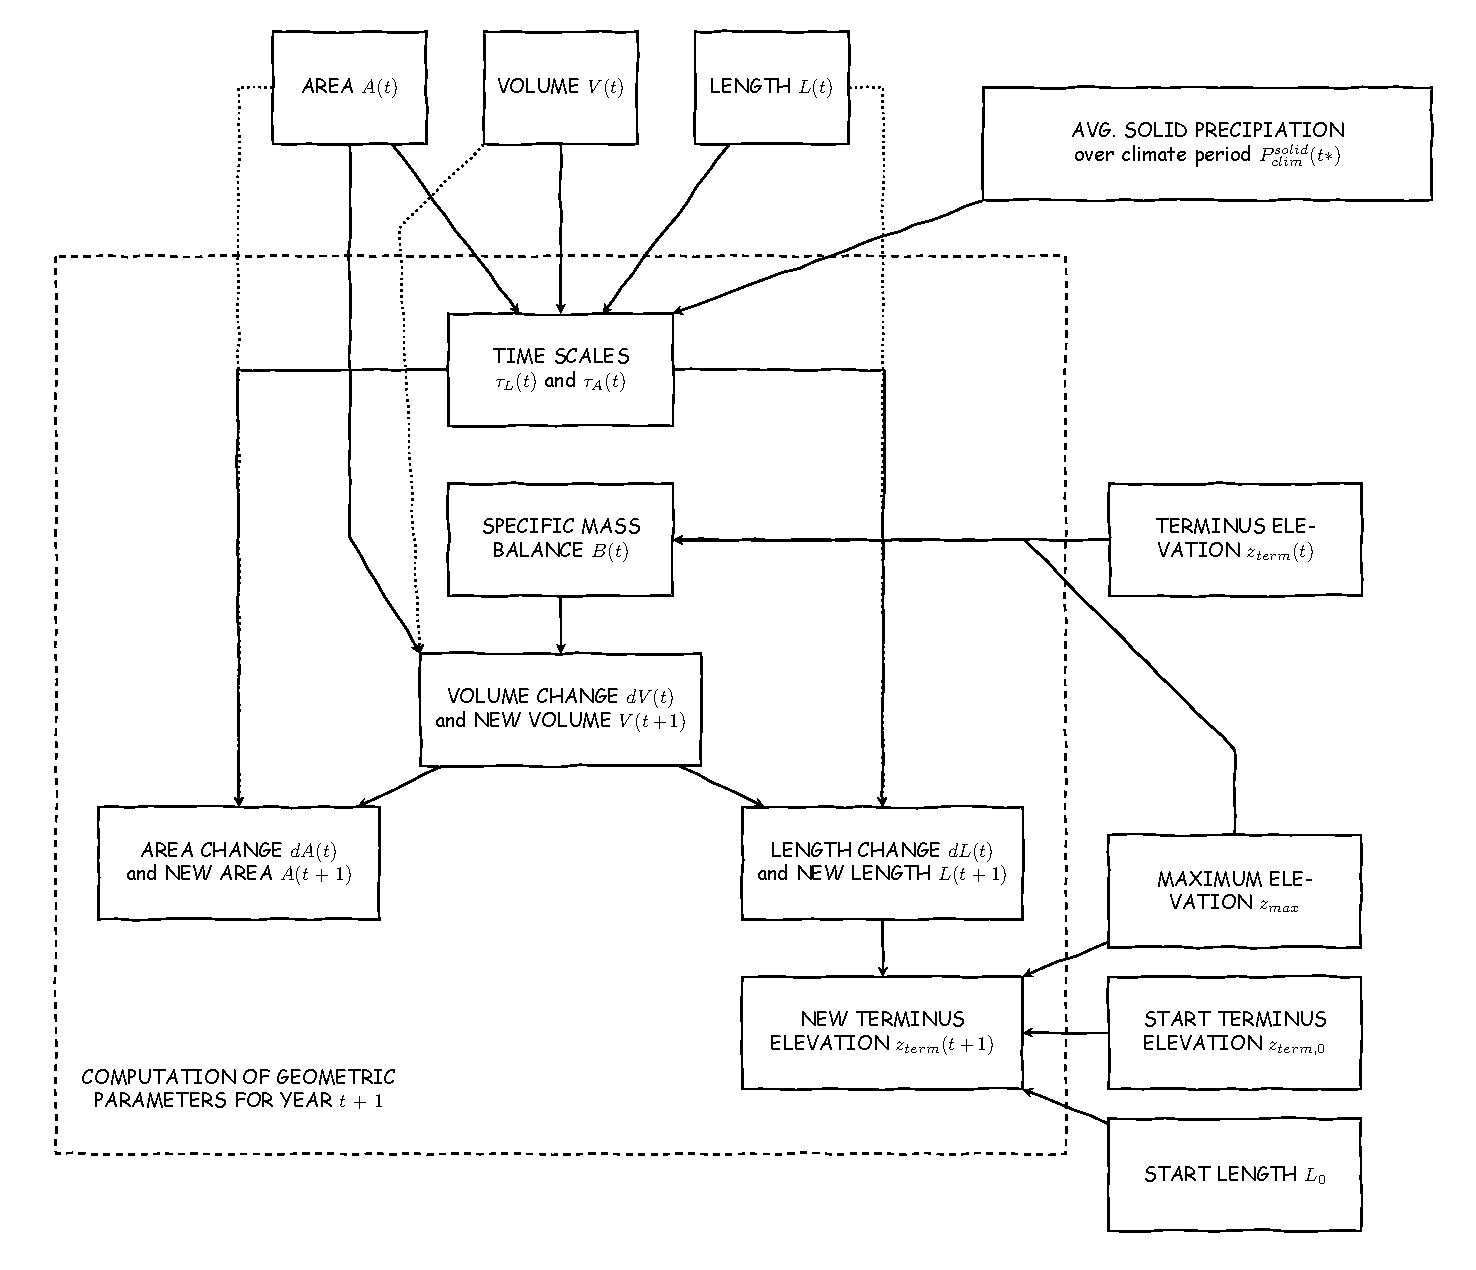
\includegraphics[width=\textwidth]{../flowchart/iterations/scaling.pdf}
            \caption{Schematic of the glacier evolution model's time stepping.}
            \label{fig:iteration-scheme}
        \end{figure}
        
        % Start area finding process ???
    
    % subsection glacier_evolution_model (end)

% section general_concepts (end)

% ==== SECTION 2 ===============================================================
\section{Implementation} % (fold)
\label{sec:implementation}

    \subsection{Mass balance models} % (fold)
    \label{sub:mass_balance_models_implementation}

        \subsubsection{Volume/area scaling mass balance model} % (fold)
        \label{ssub:volume_area_scaling_mass_balance_model_implementation}

            The \lstinline`VAScalingMassBalance` model is the implementation of the \textit{original} mass balance model by \citet{Marzeion2012b}. The model computes the mass balance of a glacier during the climate data period. The general concept is fairly similar to the \lstinline`oggm.core.massbalance.PastMassBalance` model. The main difference is, that the \vas{} mass balance model returns only one glacier wide average mass balance value, instead of point mass balance values for the different elevation bands.

            The mass balance model is initialized for a single glacier, denoted by the OGGM specific glacier directory \lstinline`gdir`. Per default, the model will use the calibrated mass balance parameters \mustar{} and \bias{} and read temperature and precipitation records from the preprocessed climate file \lstinline`climate_historical`. An alternative climate file can be used, by supplying either the filename and/or it's suffix via the parameters \lstinline`filename` and \lstinline`input_filesuffix`, repecitvely. It is possible to specify the start year and end year of the climate period (\lstinline`ys` and \lstinline`ye`), if not all available data should be used. The parameter \lstinline`repeat` controlls whether the climate period given by \lstinline`[ys, ye]` should be repeated indefinitely in a circular way.

            The \vas{} mass balance model inherits the following methods from the \lstinline`oggm.core.massbalance.MassBalanceModel` super class:
            \begin{itemize}
                \item \lstinline`get_annual_climate()` and \lstinline`get_monthly_climate()` compute and return the mass balance relevant climate information, i.e. positive air temperature at the terminus elevation in \si{\celsius} and solid precipitation amount in \si{\kg\per\square\m}, for the given year and month/year combination, respectively.
                \item \lstinline`get_annual_mb()` and \lstinline`get_monthly_mb()` compute and return the glacier wide average mass balance in \si{\m\per\s}, for the given year and month/year combination, respectively. The possible mass balance residual \bias{} is applied.
                \item \lstinline`get_specific_mb()` and \lstinline`get_monthly_specific_mb()` compute and return the glacier wide average specific mass balance in \si{mm w.e.\per yr}, for the given year and month/year combination, respectively. The possible mass balance residual \bias{} is applied.
            \end{itemize}
            All methods need the glacier terminus elevation \lstinline`min_hgt` and the maximal glacier surface elevation \lstinline`max_hgt` as parameters. The date is supplied via the \lstinline`year` parameter, using the hydrological float year convention. Given that the scaling mass balance model computes the glacier wide average mass balance, it is not possible to estimate the equilibrium line altitude. Hence, the the method \lstinline`get_ela()` is not implemented, in contrast to the \lstinline`PastMassBalance` model.
        
        % subsubsection volume_area_scaling_mass_balance_model_implementation (end)

        \subsubsection{Constant climate scenario} % (fold)
        \label{ssub:constant_climate_scenario_implementation}
            The \lstinline`ConstantMassBalance` model simulates a constant climate based on the observations averaged over a 31-year period centered on a given year \lstinline`y0`. Hence, the specific mass balance does not change from year to year. The task \lstinline`run_constant_climate(gdir, ...)` initializes a \lstinline`ConstantMassBalance` for the given glacier \lstinline`gdir` and runs for a given number of years \lstinline`nyears`. The task takes an additional temperature bias as parameters \lstinline`temp_bias`, to alter the observed climate records.

            The same idea of a constant climate is used during the mass balance calibration, solving the mass balance equation (Equation~\ref{eq:mass-balance}) for the temperature sensitivity \mustar. So per definition, \mustar{} is the temperature sensitivity to keep the glacier in equilibrium over the 31-year climate period centered around the \textit{equilibrium year} \tstar{} while neglecting a potential mass balance residual \bias. Consequentially, a \lstinline`ConstantMassBalance` model with \lstinline`y0` = \tstar{} keeps the glacier in equilibrium.
        
        % subsubsection constant_climate_scenario_implementation (end)

        \subsubsection{Random climate scenario} % (fold)
        \label{ssub:random_climate_scenario_implementation}

            Similar to the \lstinline`ConstantMassBalance` model, the \lstinline`RandomMassBalance` model is based on a 31-year period centered on a given year \lstinline`y0`. However, the mass balance years are randomly shuffled within that period. More precise, for each simulated year the model computes the specific mass balance using temperature and precipitation records from a randomly selected year within the given period. Hence, the model runs on a synthetic random climate scenario based on actual observations. A seed \lstinline`seed`' for the random generator can be supplied as parameter, to allow for reproducibility. Additionally, it is possible to choose between draws with and without replacement via the \lstinline`unique_sample` parameter.

            The task \lstinline`run_random_climate(gdir, ...)` works analogously to the task \lstinline`run_constant_climate(gdir, ...)`, using an instance of \lstinline`RandomMassBalance` model instead of the \lstinline`ConstantMassBalance` model. Hence, using the climatological period centered around \lstinline`y0` = \tstar, the model glacier should stay in an equilibrium state while underlying minor fluctuations. Supplying a positive or negative temperature bias will result in a retreating or advancing model glacier, respectively, reaching a new equilibrium after some years.
        
        % subsubsection random_climate_scenario_implementation (end)
    
    % subsection mass_balance_models_implementation (end)

    \subsection{Glacier evolution model} % (fold)
    \label{sub:glacier_evolution_model_implementation}

        The \lstinline`oggm-vas.VAScalingModel` is the implementation of the above describe glacier evolution model (see Section~\ref{sub:glacier_evolution_model}, \citet[cf.]{Marzeion2012b}) into the OGGM framework. The full source code is publicly available on \href{https://github.com/OGGM/oggm-vas}{GitHub}.

        An instance of the \lstinline`oggm-vas.VAScalingModel` class is initialized with the initial area \lstinline`area_m2_0`, the initial glacier terminus elevation \lstinline`min_hgt` and maximum glacier surface elevation \lstinline`max_hgt` and an instance of a \lstinline`oggm-vas.VAScalingMassBalance` model. Additionally, the start year of the simulation \lstinline`year_0` must be defined. Those initial values are stored as instance variables, since they are needed for later computations. Other than that, the \lstinline`oggm-vas.VAScalingModel` object stores all model parameters as instance variables for the current year it is in. This includes glacier geometries ($V$, $A$, $L$, $z_\text{min}$, $z_\text{max}$) and their changes ($\Delta V$, $\Delta A$, $\Delta L$), time scales ($\tau_A$, $\tau_L$), the mass balance model and the specific mass balance $B$, but also constants like the scaling parameters ($c_A$, $\gamma$, $c_L$, $q$) and ice density $\rho_\text{ice}$.

        To advance the glacier model, there are three different methods. The \lstinline`step()` method advances the model by one year, following the above described steps (see Section~\ref{sub:glacier_evolution_model}). The method \lstinline`run_until(year_end)` runs the model until the specified year and returns the geometric glacier parameters at the end of the model evolution (year, length, area, volume, terminus elevation and specific mass balance). Thereby, the model starts from whatever year it currently is in. It is possible to start the model run from \lstinline`year_0` with the flag \lstinline`reset`. The method \lstinline`run_until_and_store()` works analagous to the previous one, with the difference that all parameters are stored for each time step (i.e., for each year). The resulting data set is returned and possible stored to file, if a file path is give. The method \lstinline`run_until_equilibrium()` tries to run the glacier model until an equilibrium state is reached. The model runs for a fixed number of iteratrions \lstinline`max_ite`, the total elapsed time changes with the chosen time step \lstinline`ystep`. The iteration breaks, either if the glacier volume is below \SI{1}{\cubic\meter} or an equilibirum is reached. An equilibrium state is reached, if the volume change rate $|V(t) - V(t+\Delta t)|/V(t)$ falls below a given value \lstinline`rate`. Therefore, the method can only be used with a \hyperref[ssub:constant_climate_scenario_implementation]{constant climate scenario} (see Section~\ref{sub:mass_balance_models_implementation}).
    
    % subsection glacier_evolution_model_implementation (end)

% section implementation (end)


% ==== SECTION 3 ===============================================================
\section{Experimental setup} % (fold)
\label{sec:experimental_setup}
    
    % intro
    Implementing the \vas{} model is all good and well, but how does it compare to the flowline model?!
    While successfully passing the unit test is a necessity---or at least good programming practice---unit tests are only testing for coding errors and not for the physicality of the results. Nor do they answer the main research question: ``What information is gained from the use of a physical based flowline model?'' The following experiments run the newly implemented model in a variety of setting and compare it to the OGGM flowline model. The focus is on the intrinsic model behavior and its comparison to the flowline model, not on absolute ice volume estimations.

    The experiments start on the smallest scale possible, namely with a single glacier. This first test case is intended to get a feel for the model and set the stage for the following experiments. Qualitative conclusions are drawn from time series of glacier geometries in response to different equilibrium climates. Some more quantitative results are obtained from an analysis of autocorrelation and power spectral density of length change signals under a white noise climate, inspired by \citep{Roe2014}. Both analyses can only be performed on the signal of a single glacier, since mirroring oscillation of different glaciers could cancel each other out. To avoid another N-of-1 experiment, six different Alpine glaciers are investigated during this step. 
    While it may be necessary for the aforementioned experiments, it is not appropriate to apply scaling relations to a single glacier. \Vas{} should only be applied to a collection of glaciers \citep{Bahr2015}. The first regional run looks at the evolution of aggregate ice volume of all Alpine glaciers for different equilibrium climate scenarios.
    Any differences between the \vas{} model and the flowline model found above may be caused by the parameters defining the scaling relations. The parameters in question are the length timescale and area timescale for the response time scaling as well as the scaling constants and scaling exponents for the volume/length and \vas{}. A sensitivity analysis of said parameters is performed on a single glacier and on the collective Alpine glaciers.
    As a final experiment, the \vas{} model is used to estimate the potential ice melt over the coming one-hundred years for all Alpine glaciers. This is done by using todays climate in combination with a different positive temperature biases to simulate different climate scenarios.

    All the aforementioned experiments can be classified as equilibrium experiments. As most things in nature, glaciers strive toward an equilibrium condition. Such an equilibrium is reached eventually, by adjusting the glacier's geometry in reaction to changes in climatic conditions. Analyzing the behavior of a glacier model subjected to a step change in climate can be used to get insight into the dynamics of the numerical model, e.g. to estimate response times. The OGGM provides two convenient climate scenarios (or rather mass balance models) for such equilibrium experiment: the \lstinline`ConstantMassBalance` model and the \lstinline`RandomMassBalance` model. The implementation and workings of both mass balance models are described in Section~\ref{sub:mass_balance_models_implementation} (see \hyperref[ssub:constant_climate_scenario_implementation]{constant} and \hyperref[ssub:random_climate_scenario_implementation]{random} climate scenario). The hereafter detailed experiments use the HISTALP dataset \citep{Auer2007} as climate input data, with the corresponding hyper parameters (see  \href{https://oggm.org/2018/08/10/histalp-parameters/}{Mass-balance model calibration for the Alps} \citep{Dusch2018} on the OGGM blog for more information). This obviously limits the suitable glaciers to the ones inside the HISTALP domain, i.e. the Alps. The HISTALP domain corresponds to the region 11-01 of the Randolph Glacier Inventory (RGI) \citep{RGI2017,Pfeffer2014} (version 6.x) and lists 3892 glaciers.

    The following paragraph briefly lists the preprocessing tasks needed for the equilibrium runs. For a detailed description of OGGM workflow see \citet{Maussion2019} and the \href{https://docs.oggm.org}{OGGM documentation}.
    \begin{description}[noitemsep]
        \item[GIS tasks:] using the digital elevation model (DEM) from the Shuttle Radar Topography Mission (\href{http://srtm.csi.cgiar.org/}{SRTM}, \citet{Jarvis2008}) and the RGI glacier outlines to compute a local grid, compute a glacier mask, compute centerlines and corresponding catchment areas;
        \item[climate tasks:] extract the HISTALP time series for the grid point nearest to the glacier and write it in the \lstinline`climate_historical.nc` file;
        \item[mass balance calibration:] computing the glacier specific mass balance parameters \tstar{}, \mustar{} and \bias{};
        \item[inversion tasks:] running the ice thickness inversion to estimate the bed topography (needed only for the flowline model);
    \end{description}

    The actual model runs are invoked via the \lstinline`run_constant_climate` and \lstinline`run_random_climate` tasks (see Section~\ref{sub:mass_balance_models_implementation} for implementation details). The used settings depend on the intended experiment and are detailed in the following sections.

    \subsection{Single glacier test case} % (fold)
    \label{sub:single_glacier_test_case_setup}

        The first qualitative look at the \vas{} performance uses the Hintereisferner (RGI60-11.00897) as test case. This test case is intended to get a feel for the \vas{} model and set the stage for the following experiments, by comparing the two mass balance models suitable for equilibrium experiments.
        It has to be noted that \vas{} applied to single glaciers gives only an order of magnitude estimation. The scaling constant $c$ is a globally averaged value, and the relative error in scaling constant is directly proportional to the error in estimated ice volume \citep{Bahr2015}. However, a qualitative comparison between the \vas{} model and the flowline model is more practicable and meaningful for a single glacier. The model's sensitivity to its scaling parameters is investigated in Section~\ref{sec:sensitivity_experiments_results}

        % Mass balance calibration and mass balance models using the same tstar
        For this first experiment, both evolution models run with the \lstinline`ConstantMassBalance` model and the \lstinline`RandomMassBalance` model, for 1000 years each. Both mass balance models emulate an equilibrium climate to keep the glacier in its initial equilibrium state. Therefore, the mass balance models must be initialized with the climatic period centered around the equilibrium year, i.e., \lstinline`y0` = \tstar{}. As explained above, the mass balance calibration depends, among others, on the chosen \tstar{} (Section~\ref{sub:temperature_index_model}, see \hyperref[ssub:mb_calib]{Calibration of the mass balance parameters}). Hence, to run both evolution models with the identical climatic forcing, \tstar{} must be equal for both. This is done by computing the temperature sensitivity \mustar{} for both models using the same \tstar{} reference table (\lstinline`oggm_ref_tstars_rgi6_histalp.csv`, corresponding to the flowline model). Additionally, the mass balance residual must be omitted during the model run ($\beta^*$ = 0, as per the definition of \mustar{}, see Section~\ref{sub:temperature_index_model}). Each mass balance model runs three different climate scenarios defined by the temperature biases of \SI{0}{\celsius}, \SI{-0.5}{\celsius} and \SI{+0.5}{\celsius}. These runs will be referred to as \emph{equilibrium run}, run with \emph{positive mass balance bias} and run with \emph{negative mass balance bias}, respectively.
    
    % subsection single_glacier_test_case_setup (end)

    \subsection{Autocorrelation and Power spectral density} % (fold)
    \label{sub:autocorrelation_and_power_spectral_density_setup}

        The autocorrelation function of a signal measures the correlation between data points separated by any lag time $k$. Hence, the autocorrelation is a function of lag time $k$, computed as the correlation coefficient between the original signal and a lagged copy of itself. It is used find possible periodicities hidden in noisy signals and gives an estimate on how strong neighboring data points influence each other. A high autocorrelation at lag time $k$ indicates that data points that are a time $k$ apart have similar values. The autocorrelation function at lag time $k=0$ is obviously one, since any signal correlates to \SI{100}{\percent} with itself.
        The power spectral density is the Fourier transform of the autocorrelation function. The Fourier transform decomposes the signal into a spectrum of frequencies (much rather a collection of frequency bins). Hence, the power spectral density is as function of frequency. The signal's power is its energy per unit time. Thereby, the power is of unit \si{[X^2]} if the signal's unit is \si{[X]} and must not be actual physical power of unit \si{[\watt]}. The power density is the power normalized with the frequency bin width, hence the power density has the unit \si{[X^2/\hertz]} if the frequency is measured in \si{[\hertz]}. The power spectral density is used to find dominant frequencies in noisy signals.

        The autocorrelation and power spectral density are computed for the glacier length change signal, inspired by \citep{Roe2014}. To avoid another N-of-1 experiment, the behavior of the \vas{} model is compared to the flowline model for the following six Alpine glaciers:
        \begin{itemize}
            \item Hintereisferner (RGI60-11.00897), Ötztal Alps, Austria
            \item Pasterze (RGI60-11.00106), Hohe Tauern, Austria
            \item Mer de Glace (RGI60-11.03643), Mont Blanc massif, France
            \item Glacier d'Argentière (RGI60-11.03638), Mont Blanc massif, France
            \item Großer Aletschgletscher (RGI60-11.01450), Bernese Alps, Switzerland
            \item Rhonegletscher (RGI60-11.01238), Urner Alps, Switzerland
        \end{itemize}
        These glaciers are selected because of the size and notoriety, however the choice is somewhat arbitrary. All glaciers are subjected to different random (white noise) climate conditions for 10\ 000 years. The remaining settings are analogous to the single glacier test case. The \lstinline`RandomMassBalance` model is initialized around the respective \textit{equilibrium year} for each glacier (\lstinline`y0` = \tstar), whereby both evolution model use the same \tstar{} reference table.
        To increase the amount of available data, each glacier is subjected to three different climate scenarios, specified by a temperature bias of \SI{-0.5}{\celsius}, \SI{0}{\celsius} and \SI{+0.5}{\celsius}, respectively. The mass balance residual is omitted ($\beta^* = 0$). The different temperature biases lead to a large, medium an small sized glacier. The initial 1000 years are clipped, since the adjustment period could falsify the results.

        The autocorrelation function is computed using the python function \href{https://www.statsmodels.org/devel/generated/statsmodels.tsa.stattools.acf.html}{\lstinline`statsmodels.tsa.stattools.acf`} via a fast Fourier transform. The power spectral density is estimated using Welch's method. Welch's method reduces the variance in  estimated power density by time-averaging, at the cost of frequency resolution \citep[e.g.,][]{Welch1967, Proakis2007}.  The resulting 9000 data points are divided into nine time windows with a window size of 1800 datapoints and a \SI{50}{\percent} overlap. The windows are tapered using the Hann function. For details about additional parameters see the default values of the python function \href{https://docs.scipy.org/doc/scipy/reference/generated/scipy.signal.welch.html}{\lstinline`scipy.signal.welch`} which is used for computation.
    
    % subsection autocorrelation_fand_power_spectral_density_setup (end)

    \subsection{Regional runs with all Alpine glaciers} % (fold)
    \label{sub:regional_runs_with_all_alpine_glaciers_setup}
        \Vas{} applied to single glaciers gives only an order of magnitude estimation, since the scaling constant $c$ is a globally averaged value. A potential relative error in $c$ will be directly transfered to any volume estimation. Hence, \vas{} should only be applied to collections of glaciers \citep{Bahr2015}. 
        This first regional simulations over all Alpine glaciers are based on an equilibrium climate, in analogy to the single glacier test case.

        These simulations are intended to reflect the reality as good as possible. Hence, the default OGGM \hyperref[ssub:mb_calib]{mass balance calibration} is used (see Section~\ref{sub:temperature_index_model}). This means, each evolution model uses its own \tstar{} reference table (which may result in different \tstar{} for the same glacier depending on the evolution model) and the mass balance residual \bias{} is used for each run. Both evolution models run with the \lstinline`ConstantMassBalance` model and the \lstinline`RandomMassBalance` model, for 1000 years each. The mass balance models are initialized with \lstinline`y0` = \tstar{} and run with the same three different temperature biases as before (\SI{0}{\celsius}, \SI{-0.5}{\celsius}, \SI{+0.5}{\celsius}).
    
    % subsection regional_runs_with_all_alpine_glaciers_setup (end)

    \subsection{Sensitivity experiments} % (fold)
    \label{sub:sensitivity_experiments_setup}
        % introduction
        ... Before moving to the final experiments estimating future ice volume loss, it is necessary to determine the model's sensitivities. The following sensitivity analysis investigates the effects of the model-internal time scales and scaling parameters on the model behavior. Both parameter sets are specific to the scaling model, since they determine the response time scaling as well as the volume/length and \vas{}. For consistency, the sensitivity experiments are performed on Hintereisferner (RGI60-11.00897) as a single glacier test case and on all Alpine glaciers inside the HISTALP domain. For simplicity, only the \lstinline`ConstantMassBalance` model with a temperature bias of \SI{+0.5}{\celsius} is used for all runs.

        % Time scales
        The scaling model estimates glacial evolution via the implemented response time scaling. Response time scaling adjusts the yearly change in geometry in relation to the total possible change using the model-internal response time scales for length and area, $\tau_L$ and  $\tau_A$, respectively (see Section~\ref{sub:glacier_evolution_model} and \ref{sub:glacier_evolution_model_implementation} for details).
        However, the model-internal time scales are only a rough estimate and hence good possible tuning parameters. The sensitivity experiments compare the model output for different time scales, modified by a linear factor $\tau_\text{sens.} = f \cdot \tau$. Hereby, the factor $f$ is only applied to $\tau_L$, since $\tau_A$ is a linear function of $\tau_L$. The default values with $f=1$ serves as baseline. From there, the model-internal time scales are halved ($f=0.5$) and doubled ($f=2$). 

        % Scaling parameters
        The other obvious choice of tuning parameters are the scaling exponents and scaling constants. The scaling constants for volume/length and \vas{}, $c_L$ and $c_A$, respectively, can be seen as random variables. The randomness stems from the statistically similar but not identical dimensionless parameters for length, area and volume  varying from glacier to glacier. Thanks to the law of large numbers, the global scaling constants $c_L = \SI{0.0180}{\kilo\meter^{3-q}}$ and $c_A = \SI{0.0340}{\kilo\meter^{3-2\gamma}}$ are a reasonable choice for a global ice volume estimation \citep{Bahr2015}. However, those parameters may be a bad fit for certain regions and therefore need calibration.
        While the scaling constants are not constant, the scaling exponents are. The \vas{} exponent was first derived as the slope of the linear regression of volume and area observations in log-log space \citep[e.g.,][]{Chen1990}. \citet{Bahr1997b} found that their values are fixed by the underlying physics and depend only on a single set of closure conditions. The closure conditions are in turn tightly bound by observations and different common closures lead to the same results. Hence, it is strongly advised to use the global values of $q = 2.2$ and $\gamma = 1.375$  for the volume/length and \vas{}. Additionally, even with different closure conditions could be justified, the area scaling exponent is bound $1.1\dot{6} \leq \gamma \leq 1.5$ by simple geometric reasoning \citep[Section 8.2]{Bahr2015}. 

        As for the time scale sensitivity experiments, the global values of the scaling exponents serve as baseline. The next run uses custom scaling constant derived from a linear regression in log-log space but with a fixed slope corresponding to the global scaling exponents. The last run uses full custom scaling constants and exponents, again derived from a linear regression in log-log space. For reasons of simplicity, data points of volume, area and length are taken from the OGGM flowline model glaciers and not from observations. The inversion volume serves as glacier volume, the RGI area as surface area and the longest centerline as glacier length.
        
        Since a linear regression can not be computed from a single data point, the Hintereisferner test case differentiates only between global and custom scaling constants (obtained by solving the scaling relations for $c$) while using the global default scaling exponents. The following two sets of scaling parameters are used:
        \begin{enumerate}[label=(\alph*)]
            \item global (default) values of $c_L = \SI{4.551}{\meter^{3-q}}$, $q = 2.2$ for volume/length scaling and $c_A = \SI{0.191}{\meter^{3-2\gamma}}$, $\gamma = 1.375$ for \vas{}
            \item custom scaling constants $c_L = \SI{1.555}{\meter^{3-q}}$ and $c_A = \SI{0.252}{\meter^{3-2\gamma}}$ with the global and physically based scaling exponents $q = 2.2$ and $\gamma = 1.375$
        \end{enumerate}
        For comparability, the sensitivity runs on Hintereisferner (RGI60-11.00897) are setup exactly the same as the test case (see Section~\ref{sub:single_glacier_test_case_setup}). This means a fixed \textit{equilibrium year} $t^{*} = 1927$ and no mass balance residual during the run. The regional Alpine runs are setup as before (see Section~\ref{sub:regional_runs_with_all_alpine_glaciers_setup}) and use the following three sets of scaling parameters:
        \begin{enumerate}[label=(\alph*)]
            \item global (default) values of $c_L = \SI{4.551}{\meter^{3-q}}$, $q = 2.2$ for volume/length scaling and $c_A = \SI{0.191}{\meter^{3-2\gamma}}$, $\gamma = 1.375$ for \vas{}
            \item custom scaling constants $c_L = \SI{1.805}{\meter^{3-q}}$ and $c_A = \SI{0.250}{\meter^{3-2\gamma}}$ with the global and physically based scaling exponents $q = 2.2$ and $\gamma = 1.375$
            \item custom scaling constants and scaling exponents $c_L = \SI{0.244}{\meter^{3-q}}$, $q = 2.517$ for volume/length scaling and $c_A = \SI{0.117}{\meter^{3-2\gamma}}$, $\gamma = 1.441$ for \vas{}
        \end{enumerate}

        Disclaimer: As already mentioned, this work is focused on the model behavior much rather than an absolute ice volume estimation. While scaling constants and exponents based in observations would be preferable, the values of the custom scaling parameters are less important as long as the are different from the global values. In fact, the sensitivity experiment could easily be conducted with a set of fabricated exponents. For the same reason, it is inconsequential that scaling exponents derived from a numerical model may differ depending on the model's closure conditions \citep[Section 8.9]{Bahr2015}. It is hereby noted that this potential source for errors is acknowledged, and the flowline model is not tested for its closure conditions. While the custom scaling exponents lie within the range of physical sensible values, finding closure conditions supporting the computed values would go (far) beyond the scope of this work.

    % subsection sensitivity_experiments_setup (end)

    \subsection{Commitment runs} % (fold)
    \label{sub:commitment_runs_setup}
        One of the easiest ways of estimating future glacial evolution are so called \textit{commitment runs}.
        The name stems from the \textit{commitment} to a given climate, which is then held constant for the entire run. For example, applying the current climate to the current glaciers for the next, say, 100 years, would give a---naively optimistic---lower bound of the expected glacial retreat. As for the first regional run, ... % TODO

        While a climate scenario with yearly fluctuations is more physical than a completely constant climate, the resulting ice volume changes are comparable (see Section~\ref{sub:time_series_results}). Which is why, the following experiments can be limited to the \lstinline`ConstantMassBalance` model without any loss of information. For a more tangible experiment, the \lstinline`ConstantMassBalance` model is initialized with todays climate. Todays climate is assumed to be the average over the most recent 31 years. For the HISTALP dataset this corresponds to the period from 1984 to 2014 with \lstinline`y0 = 1999`. Since we live in a period of global warming, additional positive temperature biases of \SI{0}{\celsius}, \SI{+0.5}{\celsius} and \SI{+1.5}{\celsius} are used. Again, the default OGGM \hyperref[ssub:mb_calib]{mass balance calibration} is used assuring the most physical outcome.
    
    % subsection commitment_runs_setup (end)

% section experimental_setup (end)
\newpage
\thispagestyle{plain}


% ==== CHAPTER 3 ===============================================================
% ---- set some counters to zero:
\setcounter{equation}{0}
\setcounter{table}{0}
\setcounter{figure}{0}
% ---- include tex-file:
%!TEX root = thesis.tex
\chapter{Results}\label{chap:results}
\thispagestyle{plain}

  The following chapter provides all findings from the different experiments detailed in Section~\ref{sec:experimental_setup}. Starting with quantitative results from a single glacier test case, to time series analysis via an ACF and PSD, to a sensitivity analysis of the scaling parameters, and finishing with regional runs for the entire European Alps.

  For all experiments except the sensitivity analysis, the \vas{} is evaluated in comparison to the flowline model. While this gives insights into the drawbacks of simple models and benefits of explicit ice physics, no accuracy assessment can be made without comparison to observational data.

  \section{Single glacier test case} % (fold)
  \label{sec:single_glacier_test_case_results}

    This first test case is intended to get a feel for the \vas{} model and set the stage for the following experiments. The model simulates the evolution of the Hintereisferner (RGI60-11.00897) over 1000 years for three different climate scenarios: an equilibrium climate, and a positive and a negative step change in climate, defined by a temperature bias of \SI{\pm0.5}{\celsius}. Additionally, two different mass balance models are used. The \lstinline`ConstantMassBalance` model simulates a perfectly constant climate and the \lstinline`RandomMassBalance` introduces random year-to-year variability, as the names may suggest. Result are compared to the flowline model. For details about the experimental setup see Section~\ref{sub:single_glacier_test_case_setup}.

    \begin{tldrbox}[Single glacier test case]{tldr:hintereisferner_test_case_results}
      \item Both evolution models produce the same qualitative results, advancing under colder climates and shrinking under warmer climates. The temporal correlation between both models under a random climate is satisfying.
      \item The \vas{} model drastically underestimates changes in glacier geometry compared to the flowline model (up to four times). For example, the relative volume changes for the run with positive mass balance bias amount to $\SI{+17}{\percent}$ for the \vas{} model and $\SI{+71}{\percent}$ for the flowline model. 
      \item The \vas{} does not account for the mass-balance-elevation feedback and therefore produces highly symmetrical results between the positive and negative step change in air temperature. This symmetry can also be seen in the e-folding response times.
      \item The e-folding response times are much shorter for the \vas{} model. For example, the volume response times for the run with positive mass balance bias amount to $\SI{39}{\year}$ for the \vas{} model and $\SI{139}{\year}$ for the flowline model. 
      \item The \vas{} model does not show an asymptotic adjustment but behaves more like a damped harmonic oscillator, whereby the model-internal time scale acts as damping factor.
    \end{tldrbox}

    % overall impression
    The \vas{} model behaves as expected and produces the same qualitative results as the flowline model. The model glacier stays in an approximate equilibrium using the climate around \tstar, and decreases and increases in size for a positive and negative temperature bias of \SI{\pm0.5}{\celsius}, respectively. However, the \vas{} model underestimate changes in geometry compared to the flowline model. This is true for both the constant and random climate scenario, whereby the \lstinline`RandomMassBalance` model, with its year-to-year variations, produces more short term variability (most obviously). Figure~\ref{fig:hintereisferner} shows the time series for ice volume, surface area and glacier length for all climate scenarios and both evolution models.

    % temporal correlation between VAS and flowline
    The modeled glacier advances and retreats forced by the random climate scenarios show a weak but highly significant correlation between the two evolution models (with correlation coefficients $0.34 \leq r \leq 0.58$ and p-values of $p \ll 0.01$). Given that the implementations of the mass balance models are almost identical between the \vas{} model and the flowline model, this is the first indication that the differences must arise from the geometry models. For both models, the ice volume exhibits the highest year-to-year variability, since volume changes happen instantaneously, i.e., over a single time step. The changes in surface area and glacier length are smoother, accounting for the glacier's response time. However, the flowline model shows generally less short term variabilities but stronger long term variabilities than the \vas{} model, indicating longer response times. This assumption is backed by the model behavior under the constant climate scenarios. Qualitatively speaking, the flowline model takes longer to reach a new equilibrium (about 400 years) than the \vas{} model (about 200 years). A quantitative analysis of the response times follows after the evaluation of the equilibrium values. 

    % Equilibrium values
    % ------------------

    % segue and introduction
    For the following discussion about the new equilibrium values, only the constant climate scenarios are considered (if not stated otherwise). It is assumed that the model glacier has reached a new equilibrium 1000 years after the climate perturbation. Hence, the equilibrium values are taken as the final values at year \lstinline`t = 1000`. This assumption seems valid, given that the fluctuation of volume, area and length are in the order of only \SI{0.01}{\percent}\footnotemark{} over the last 200 years of the simulations.
    \footnotetext{The fluctuations are computed as the relative difference between minimum and maximum value during that period. The relative difference between two values $a$ and $b$ refers to their absolute difference relative to the average between them $\left|\frac{a-b}{(a+b)/2}\right|$.}
    Table~\ref{tab:hintereisferner_equilibrium_values} shows all new equilibrium values in response to the positive and negative step changes in climate. Percentage values refer to the normalized glacier geometries to their respective initial values, which facilitates the comparison.
    
    % underestimation
    The most apparent result is that the \vas{} model underestimates all changes in glacier geometry compared to the flowline model. While the \vas{} model estimates a volume change of \SI{+17}{\percent} and \SI{-15}{\percent}, the flowline estimates \SI{+72}{\percent} and \SI{-42}{\percent}, for the negative and positive temperature perturbation, respectively. In other words, the flowline glacier grows more than four times larger and shrinks more than two and a half times smaller than the \vas{} glacier.
    The changes in surface area are slightly less underestimated, with values of \SI{+12}{\percent} and \SI{-11}{\percent} for the \vas{} model and \SI{+33}{\percent} and \SI{-23}{\percent} for the flowline model. The glacier length of the \vas{} model does hardly change at all. The year-to-year changes of glacier length estimated by the \vas{} model range between \SI{-11}{\meter} and \SI{+8}{\meter}, corresponding to a maximal change of \SI{2}{\percent} of the initial values. This results in a total length change of \SI{\pm7}{\percent} for the \vas{} model over the entire simulation, which is roughly five to six times less than the changes of \SI{+44}{\percent} and \SI{-39}{\percent} for the flowline model. The continuous length records for Hintereisferner from 1939 to 2003 \citep{Leclercq2014} show an average yearly absolute length change of $26\pm{}\SI{21}{\meter}$ (mean $\pm$ standard deviation) and a maximum of over \SI{100}{\meter}. That amounts to an maximum observed yearly length changes of \SI{1.6}{\percent} in relation to the glacier length of \SI{6.9}{\kilo\meter} in 2003. It seems that the values of relative length change of the \vas{} are comparable to observations, the absolute values, however, are far too low. This is the another indication that the \vas{} model cannot resolve all the same processes as a dedicated ice physics models can.
    
    % symmetry
    The changes in glacier geometries produces by the \vas{} model are highly symmetrical. Absolute changes ice volume, surface area and glacier length differ by a maximum of \SI{7}{\percent}, \SI{3}{\percent}, and \SI{2}{\percent}, respectively, between the run with positive and negative mass balance perturbation\footnote{The percentages correspond to the relative difference, as explained above}.
    Again, this cannot be explained by the mass balance models. The climate scenarios used for this experiment are all based on an equilibrium climate. If the input climate is not altered by a temperature bias, the model glacier will stay in its equilibrium state under the constant climate scenario. Under a random climate scenario the model glacier will show some year-to-year variability, but still fluctuation around the same equilibrium values. This specific equilibrium mass balance can be approximated as a linear function of temperature bias (with $r^2 > \SI{99.9}{\percent}$), for small enough temperature biases between \SI{-1}{\celsius} and \SI{+1}{\celsius}. Thereby, the slopes of the linear functions and consequentially the initial specific mass balance are almost identical between the \vas{} and flowline model: \SI{+309}{\milli\meter\waterequivalent\per\year} and \SI{-320}{\milli\meter\waterequivalent\per\year} for the \vas{} model and \SI{+307}{\milli\meter\waterequivalent\per\year} and \SI{-323}{\milli\meter\waterequivalent\per\year} for the flowline model. The initial mass balance values are quite symmetrical for both evolution models and can, therefore, not be the cause of the \vas{} model's symmetric equilibrium results.
    However, since this study looks for benefits of a dedicated ice physics model rather than flaws of the \vas{} model, the question should be “What allows the flowline model to produces asymmetric results?”. % the question should not be “What makes the \vas{} model results symmetric?” but much rather
    And the answer is the mass-balance-elevation feedback. The flowline model continuously adjusts the surface elevation of each grid cell and passes the elevation information onto the mass balance model\footnote{Implementation note: the mass balance feedback can be adjusted via the \lstinline`mb_elev_feedback` parameter of the \lstinline`FlowlineModel` class}. Suppressing the mass-balance-elevation feedback for the flowline model run results in a volume change of \SI{+38}{\percent} and \SI{-34}{\percent}. These results are symmetric and lower than with mass-balance-elevation feedback in place. The relative changes in ice volume are reduced to about twice the values produces by the \vas{} model.
    % segue and introduction of next section
    It has been shown, that the responses of the \vas{} model and the flowline model to a step change in climate are qualitatively similar but do not compare quantitatively. While the absolute equilibrium values are still in the same order of magnitude, they differ substantially. But what about the time domain? The following paragraphs look at temporal characteristics of the glacier model's response.

    % Time scales
    % -----------

    % time scales computed by the vas model
    The implementation of the \vas{} model includes the corresponding response time scaling to estimate temporal changes (see Section~\ref{sub:glacier_evolution_model_implementation}). For a proper response time scaling, the length response time scale $\tau_L$ and the area response time scale $\tau_A$ must be estimated. The length response time scale can be estimated as ratio between ice volume and mass turnover \citep{Johannesson1989}, the area response time scale then follows from geometric considerations. The model-internal time scales computed for the Hintereisferner under a constant equilibrium climate amount to $\tau_L \approx \SI{38}{\year}$ and $\tau_L \approx \SI{12.5}{\year}$. Those values are rather low compared to other findings of $\tau_L \approx \SI{100}{\year}$ \citep{Greuell1992, Schuster2020}. However, it is possible that the used time scales are merely model parameters and do not correspond to the typically used e-folding time scales.
    
    % e-folding time scales
    % The flowline model has no inherent measure for a glacier's time scale.
    Processes evolving exponentially to an equilibrium can be characterized by their e-folding response time. The assumption that a glacier's geometry changes exponentially is valid for small enough perturbations in climate. The e-folding response time is computed as the time after which the initial difference between a glacier's geometric property (such as ice volume, surface area or glacier length) and its new equilibrium value has decreased by a factor of $1-\mathrm{e}^{-1}\approx\SI{63}{\percent}$. For comparability, e-folding time scales are computed for both evolution models and all geometric properties. The values can be found in Table~\ref{tab:hintereisferner_time_scales}.
    As was to be expected, volume response times $\tau_V$ are smallest, followed by $\tau_A$ and $\tau_L$. As already qualitatively estimated above, the \vas{} model adjust between two times and six times faster to the temperature perturbation of \SI{\pm0.5}{\celsius} than the flowline model. This is especially visible for the growing glacier, where the flowline model takes almost \SI{120}{\year} longer to reach a new equilibrium than the \vas{} model does ($\tau_{V,\text{fl}}=\SI{142}{\year}$ vs. $\tau_{V,\text{vas}}=\SI{24}{\year}$).
    
    % symmetry
    The results of the \vas{} model are again very symmetric between the positive and negative temperature perturbation. The \vas{} e-folding time scales range within \SI{9}{\percent} of each other, while the flowline response time scales vary up to \SI{55}{\percent}\footnotetext{The percentages correspont to the relative difference, as explained above.}. Suppressing the mass-balance-elevation feedback for the flowline model results in similarly symmetric result.
    % oscillation
    It has to be noted, that the length e-folding response time for the \vas{} model $\tau_{L,\text{vas}}\approx\SI{55}{\year}$ is over twenty years (\SI{\approx 30}{\percent}) longer than the model-internal time scale.
    However, the \vas{} model does not show an asymptotic or exponential adjustment. The adjustment of glacier geometries looks like the signal of an underdamped oscillator, with a strongly discernible overshoot. The damping factor seems to be controlled by the model-internal time scale, which could allow for an additional tuning parameter. A closer look at this oscillatory behavior is provided in Section~\ref{sec:sensitivity_to_model_internal_time_scales_results}

    % scaling for single glacier, sensitivity to scaling constant
    While Hintereisferner is not representative for all Alpine glaciers, the same experiment performed on other single glaciers yields similar results (see Appendix~\ref{appendix_A}). For some glaciers (e.g., Mer de Glace, Glacier d'Argentière) the change in relative ice volume is comparable between the two evolution models. However, this is merely a mathematical artifact, since the initial ice volume estimated by the scaling relation is much smaller than the one from the numerical ice thickness inversion. The absolute values of ice volume and ice volume change are still drastically underestimated by the \vas{} model. Unlike ice volume and glacier length, the initial surface area is equivalent for both models. This generally results in better agreement of estimated final equilibrium areas, even though the glacier areas simulated by the \vas{} model show far more and stronger fluctuations under random climates.
    Anyway, all of those observations are not robust, since scaling relations are developed to work best on a global or at least a regional scale. The scaling constant $c$ is a random variable which can vary drastically from glacier to glacier. It is possible that the global mean value of $c=\SI{0.034}{\kilo\meter^{3-2\gamma}}$ is a bad fit for the characteristics of Hintereisferner (or any other single glacier). A detailed look at the model's sensitivity to the scaling constant is provided in Section~\ref{sec:sensitivity_to_scaling_parameters_results}.

    
    % Table showing the Hintereisferner equilibrium values, geometries as columns including initial values
    \begin{table}[htp]
      \centering
      \small
      \ra{1.4}

      \caption{Hintereisferner (RGI60-11.00897) equilibrium values after 1000 years of model evolution in response to a step change in climate of $\Delta T = $\SI{\pm0.5}{\celsius} relative to the average climate between 1912 and 1942. Percentage values in parenthesis indicate normalized changes in respective to their initial values.}
      \label{tab:hintereisferner_equilibrium_values}
      
      \begin{tabular}{@{}rcrlcrlcrl@{}}
        \toprule
        {} & \phantom{a} & \multicolumn{2}{c}{\textbf{Length [\si{\kilo\meter}]}} & \phantom{a} & \multicolumn{2}{c}{\textbf{Area [\si{\square\kilo\meter}]}} & \phantom{a} & \multicolumn{2}{c}{\textbf{Volume [\si{\cubic\kilo\meter}]}} \\
        \midrule
        \textbf{Initial values} \\
        V/A scaling & \phantom{a} & 4.89 & & \phantom{a} & 8.04 & & \phantom{a} & 0.60 & \\
        Flowline & \phantom{a} &  6.90 & & \phantom{a} & 8.04 & & \phantom{a} & 0.80 & \\
        $\bm{\Delta T}$\textbf{ = \SI{-0.5}{\celsius}} \\
        % \cmidrule{1-10}
        V/A scaling & \phantom{a} & 5.25 & (\SI{+7}{\percent}) & \phantom{a} & 8.98 & (\SI{+12}{\percent}) & \phantom{a} & 0.70 & (\SI{+17}{\percent}) \\
        Flowline & \phantom{a} &  9.80 & (\SI{+42}{\percent}) & \phantom{a} & 10.64 & (\SI{+33}{\percent}) & \phantom{a} &  1.38 & (\SI{+72}{\percent}) \\
        \addlinespace
        $\bm{\Delta T}$\textbf{ = \SI{+0.5}{\celsius}} \\
        % \cmidrule{1-10}
        V/A scaling & \phantom{a} & 4.54 & (\SI{-7}{\percent}) & \phantom{a} & 7.12 & (\SI{-11}{\percent}) & \phantom{a} & 0.50 & (\SI{-15}{\percent}) \\
        Flowline & \phantom{a} &   3.80 & (\SI{-45}{\percent}) & \phantom{a} & 6.16 & (\SI{-23}{\percent}) & \phantom{a} & 0.46 & (\SI{-42}{\percent}) \\
        \bottomrule
      \end{tabular}
    \end{table}

    % Table showing the e-folding time scales for Hintereisferner, time scales as columns
    \begin{table}[htp]
      \centering
      \small
      \ra{1.4}

      \caption{e-folding time scales for Hintereisferner (RGI60-11.00897) in response to a step change in climate of $\Delta T = $\SI{\pm0.5}{\celsius} relative to the average climate between 1912 and 1942. Time scales are computed for changes in ice volume, surface area and glacier length, denoted as $\tau_V$, $\tau_A$ and $\tau_L$, respectively.}
      \label{tab:hintereisferner_time_scales}
      
      \begin{tabular}{@{}rcrcrcr@{}}
        \toprule
        {} & \phantom{a} & $\bm{\tau_L}$ \textbf{[\si{\year}]} & \phantom{a} & $\bm{\tau_A}$ \textbf{[\si{\year}]} & \phantom{a} & $\bm{\tau_V}$ \textbf{[\si{\year}]} \\
        \midrule
        $\bm{\Delta T}$\textbf{ = \SI{-0.5}{\celsius}} \\
        % \cmidrule{1-10}
        V/A scaling & \phantom{a} & 55 & \phantom{a} & 36 & \phantom{a} & 24 \\
        Flowline & \phantom{a} &  184 & \phantom{a} & 160 & \phantom{a} & 142 \\
        \addlinespace
        $\bm{\Delta T}$\textbf{ = \SI{+0.5}{\celsius}} \\
        % \cmidrule{1-10}
        V/A scaling & \phantom{a} & 52 & \phantom{a} & 33 & \phantom{a} & 22 \\
        Flowline & \phantom{a} & 118 & \phantom{a} & 111 & \phantom{a} & 80 \\
        \bottomrule
      \end{tabular}
    \end{table}

    % Figure showing Hintereisferner time series plots - on page
    \begin{figure}[p]
      \centering

      % VAS volume
      \begin{subfigure}[b]{0.476\textwidth}
        \caption{\Vas{} model, relative ice volume}
        \label{fig:hintereisferner:volume_vas}
        \centering
        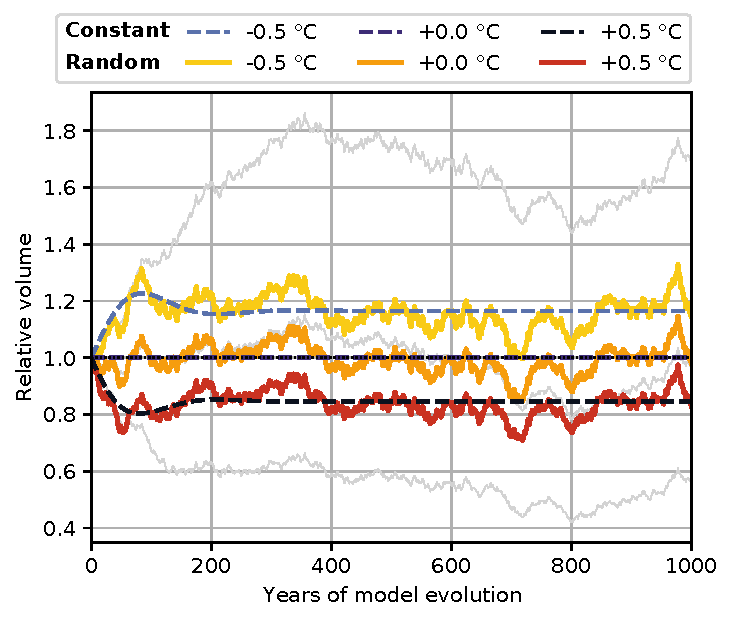
\includegraphics[width=\textwidth]{../plots/final_plots/time_series/single_glaciers/volume_norm_vas_Hintereisferner.pdf}
      \end{subfigure}
      \hfill
      % Flowline volume
      \begin{subfigure}[b]{0.476\textwidth}
        \caption{Flowline model, relative ice volume}
        \label{fig:hintereisferner:volume_fl}
        \centering
        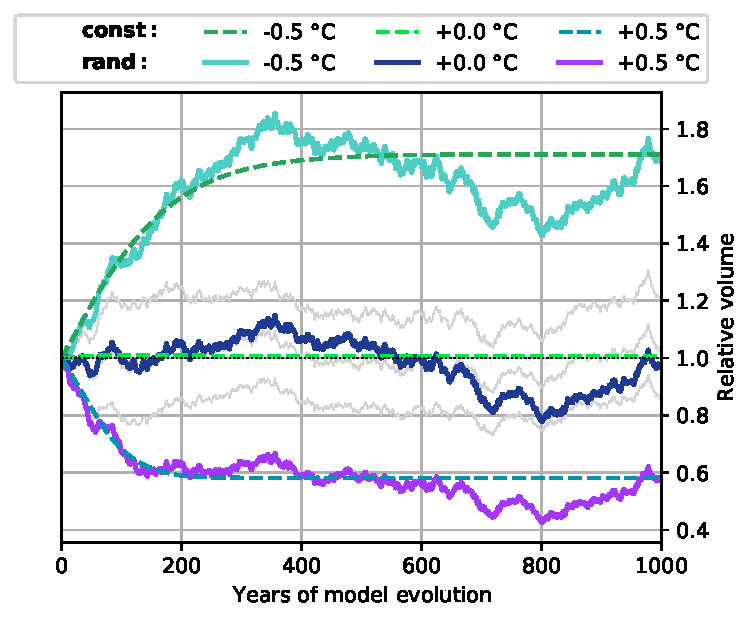
\includegraphics[width=\textwidth]{../plots/final_plots/time_series/single_glaciers/volume_norm_fl_Hintereisferner.pdf}
      \end{subfigure}

      % VAS area
      \begin{subfigure}[b]{0.476\textwidth}
        \caption{\Vas{} model, relative surface area}
        \label{fig:hintereisferner:area_vas}
        \centering
        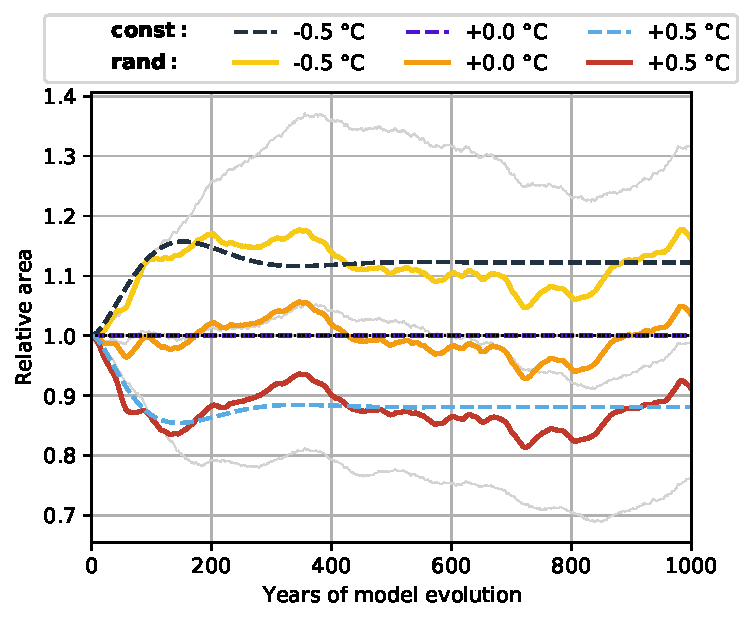
\includegraphics[width=\textwidth]{../plots/final_plots/time_series/single_glaciers/area_norm_vas_Hintereisferner.pdf}
      \end{subfigure}
      \hfill
      % Flowline area
      \begin{subfigure}[b]{0.476\textwidth}
        \caption{Flowline model, relative surface area}
        \label{fig:hintereisferner:area_fl}
        \centering
        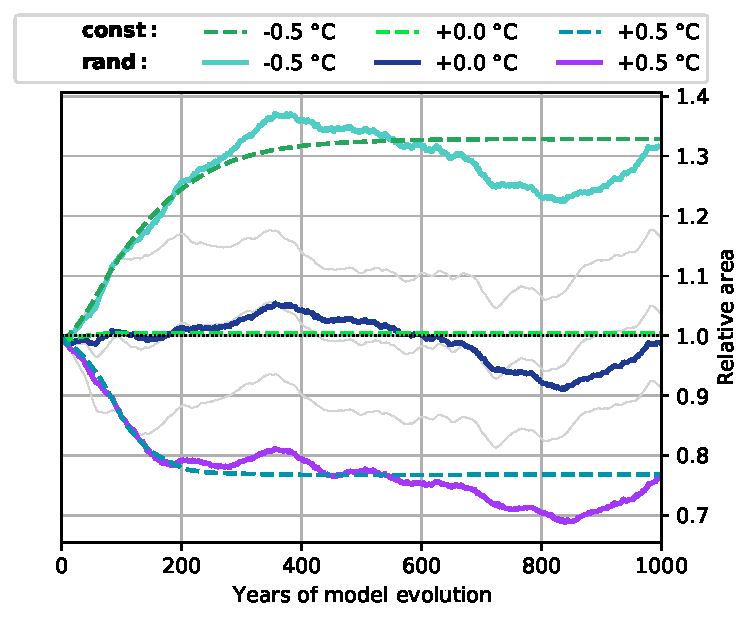
\includegraphics[width=\textwidth]{../plots/final_plots/time_series/single_glaciers/area_norm_fl_Hintereisferner.pdf}
      \end{subfigure}

      % VAS length
      \begin{subfigure}[b]{0.476\textwidth}
        \caption{\Vas{} model, relative glacier length}
        \label{fig:hintereisferner:length_vas}
        \centering
        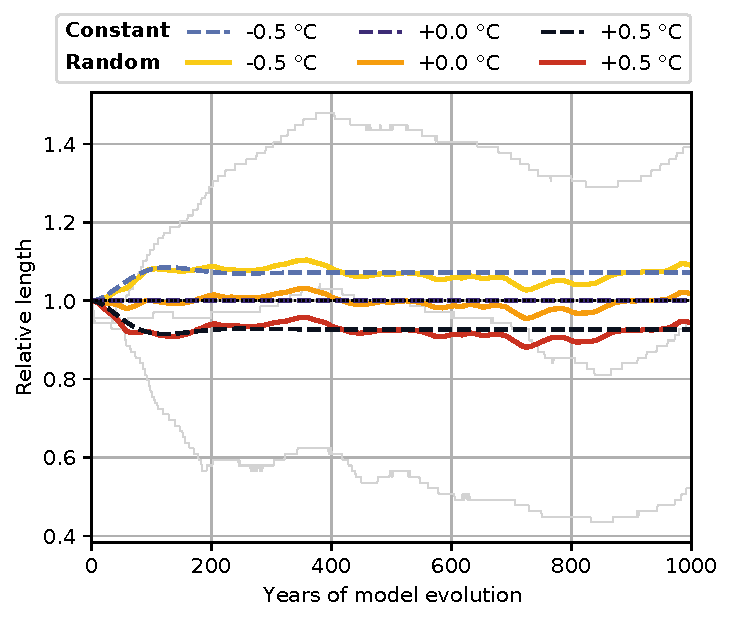
\includegraphics[width=\textwidth]{../plots/final_plots/time_series/single_glaciers/length_norm_vas_Hintereisferner.pdf}
      \end{subfigure}
      \hfill
      % Flowline length
      \begin{subfigure}[b]{0.476\textwidth}
        \caption{Flowline model, relative glacier length}
        \label{fig:hintereisferner:length_fl}
        \centering
        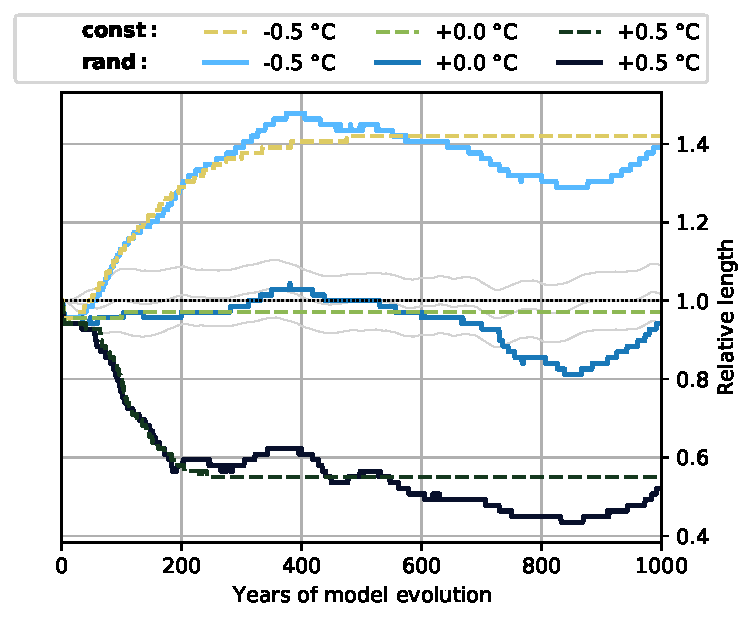
\includegraphics[width=\textwidth]{../plots/final_plots/time_series/single_glaciers/length_norm_fl_Hintereisferner.pdf}
      \end{subfigure}
      
      \caption{Temporal evolution of ice volume in (\subref{fig:hintereisferner:volume_vas}) and (\subref{fig:hintereisferner:volume_fl}), surface area in (\subref{fig:hintereisferner:area_vas}) and (\subref{fig:hintereisferner:area_fl}) and glacier length in (\subref{fig:hintereisferner:length_vas}) and (\subref{fig:hintereisferner:length_fl}) for Hintereisferner (RGI60-11.00897). The shown values area normalized with their respective initial values. The left panels show the result of the \vas{} model, the right panels show the results of the flowline model. Solid lines represent the random climate scenarios, while dashed lines represent the constant climate scenarios. All climate scenarios are based on an equilibrium climate. The applied temperature biases of \SI{-.5}{\celsius}, \SI{0}{\celsius} and \SI{+.5}{\celsius} are color coded, see legend for details. The dotted line indicates the initial volume. The light gray lines represent the volume evolutions of the other model, to facilitate comparisons.}
      \label{fig:hintereisferner}
    \end{figure}

    While the

  % section single_glacier_test_case_results (end)


  \section{Autocorrelation function and Power spectral density} % (fold)
  \label{sec:autocorrelation_and_power_spectral_density_results}
    
    % intro
    The autocorrelation function (ACF), partial autocorrelation function (PACF) and power spectral density (PSD) give insight into the periodicity and dominant frequencies of a given signal. The length signals of different  glaciers, modeled as response to different constant climate scenarios with random year-to-year variabilities, are investigated in this section (see Figure~\ref{fig:random_length}). The experiment is setup in analogy to the single glacier test case, since ACF, PACF and PSD are only meaningful for time series of a single glacier. To avoid a N-of-1 experiment, five more individual glaciers are investigated, namely the Pasterze, Mer de Glace, Glacier d'Argentière, Aletschgletscher and Rhonegletscher. All glaciers are subjected to different random (white noise) climate conditions for 20\ 000 years. The spinup period during which the glaciers adjust to the different climate is clipped, which leaves three different sizes of the same glacier. Hence, the temperature bias can be seen as a label for glacier size rather than climatic conditions. For details about the experimental setup see Section~\ref{sub:autocorrelation_and_power_spectral_density_setup}. The ACF for lag times up to 200 years is shown in Figure~\ref{fig:acf}, the PACF for lag times up to 20 years in Figure~\ref{fig:pacf} and the PSD in Figure~\ref{fig:psd}.

    Figure~\ref{fig:random_length} shows the length anomalies with respect to the equilibrium value for the arbitrarily chosen period between 8000 and 12\,000 years. This allows to formulate some first qualitative conclusions. The overlaid length changes seem to be in good agreement between the \vas{} and the flowline model. While correlations may be high, the difference in absolute length fluctuations is already apparent by looking at the y-scales (left for the flowline model and right for the \vas{} model). While the length changes estimated by the \vas{} model are all in the order of \SI{\pm200}{\meter} (except \SI{\pm500}{\meter} for the Pasterze, see Figure~\ref{fig:random_length:pasterze}), the flowline model predicts fluctuations between \SI{\pm500}{\meter} for the Rhonegletscher (Figure~\ref{fig:random_length:rhonegletscher}) and \SI{\pm2500}{\meter} for the Aletschgletscher (Figure~\ref{fig:random_length:großer_aletschgletscher}). Furthermore, different sizes of the same glacier show similar but noticeable different length fluctuation under the flowline model, while there seems to be little to no differences under the \vas{} model. However, these first findings are only based on the visual inspection of a temporally limited subsample and are further investigated and quantified in the following sections.

    \subsection{Power spectral density} % (fold)
    \label{sub:power_spectral_density_results}

      % intro and general
      % low pass filter
      Glaciers act as low-pass filters for the natural climate variability. A low pass filter passes lower frequencies while attenuating higher frequencies, which results in a characteristic PSD curve. Figure~\ref{fig:psd} shows the PSD of glacier lengths for the six glaciers mentioned above. The power density stays in a constant range for frequencies up to \SI{3e-3}{\per\year} (corresponding to signals with a period of over 300 years) before decreasing with increasing frequency. This makes intuitive sense, since changes in glacier length are mainly driven by long term climatic trends and less by inter-annual variabilities in the climatic forcing. A single year with low temperatures and strong (cold season) precipitation has less impact on the glacier size than a decade of slightly above-average temperatures.
      % higher power density of flowline model
      While the overall shape of the PSDs are similar for the \vas{} model and the flowline model, there are some key differences. As seen before, the length changes estimated by the \vas{} model are smaller compared to the flowline model. Hence, the overall power of the flowline model is higher across all frequencies. In agreement with the symmetric behavior discussed before, the PSDs of the \vas{} model are practically identical for different sizes of the same glacier. The PSDs based on the flowline length are less coherent between different sizes of the same glacier, whereby there is no discernible relation between shape of PSD and glacier size.
      % power density for high frequencies
      Additionally, the flowline model shows a rather constant power density for lower frequencies. This is due to the discrete changes in glacier length of the flowline model, whose resolution depends on the grid size (\SI{100}{\meter} in this case). The \vas{} model length is a continuous variable, resulting in a constantly decreasing power density.
      % slope?
      While the absolute values are different, the slope of the PSDs are almost identical between \vas{} and flowline model for medium frequencies up to about \SI{3e-2}{\per\year} (corresponding to signals with a period of over 30 years). This indicates that the breakdown of energy from larger to smaller scales happens at similar rates for both models (cp. the energy cascade for turbulent flows, e.g., \cite{Wyngaard2010}).

      % Random length plots
      \begin{figure}[htp]
        \centering
        \begin{subfigure}[b]{0.48\textwidth}
          \caption{RGI60-11.00897 - Hintereisferner}
          \label{fig:random_length:hintereisferner}
          \centering
          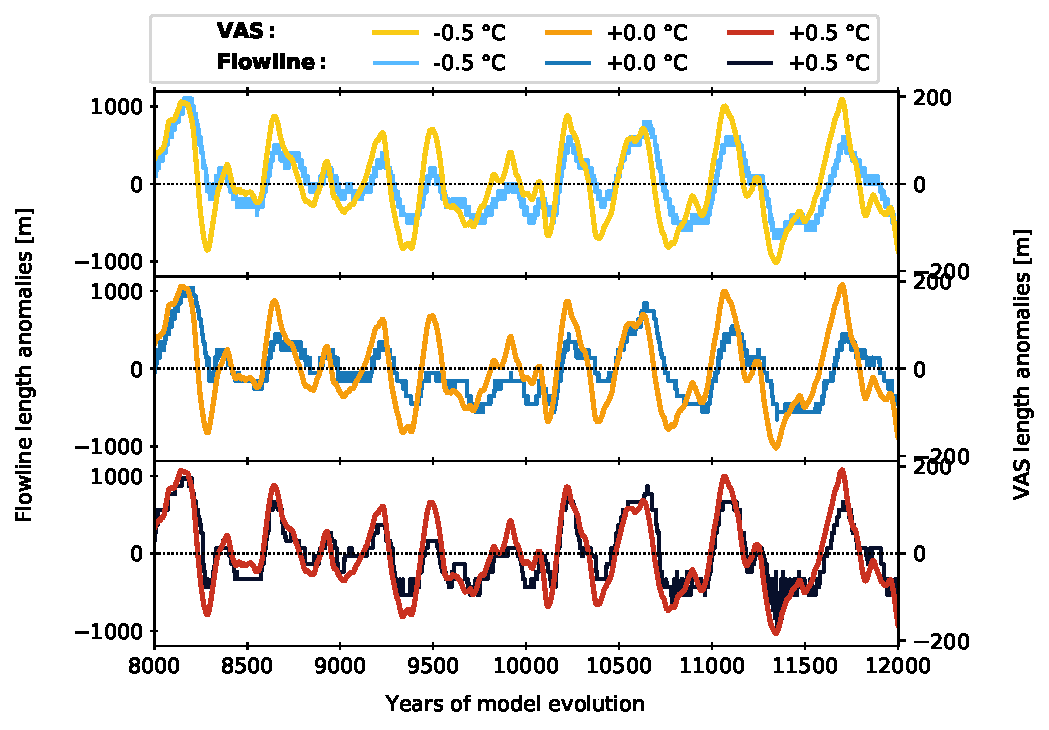
\includegraphics[width=\textwidth]{../plots/final_plots/random_length/Hintereisferner.pdf}
        \end{subfigure}
        \hfill
        \begin{subfigure}[b]{0.48\textwidth}
          \caption{RGI60-11.00106 - Pasterze}
          \label{fig:random_length:pasterze}
          \centering
          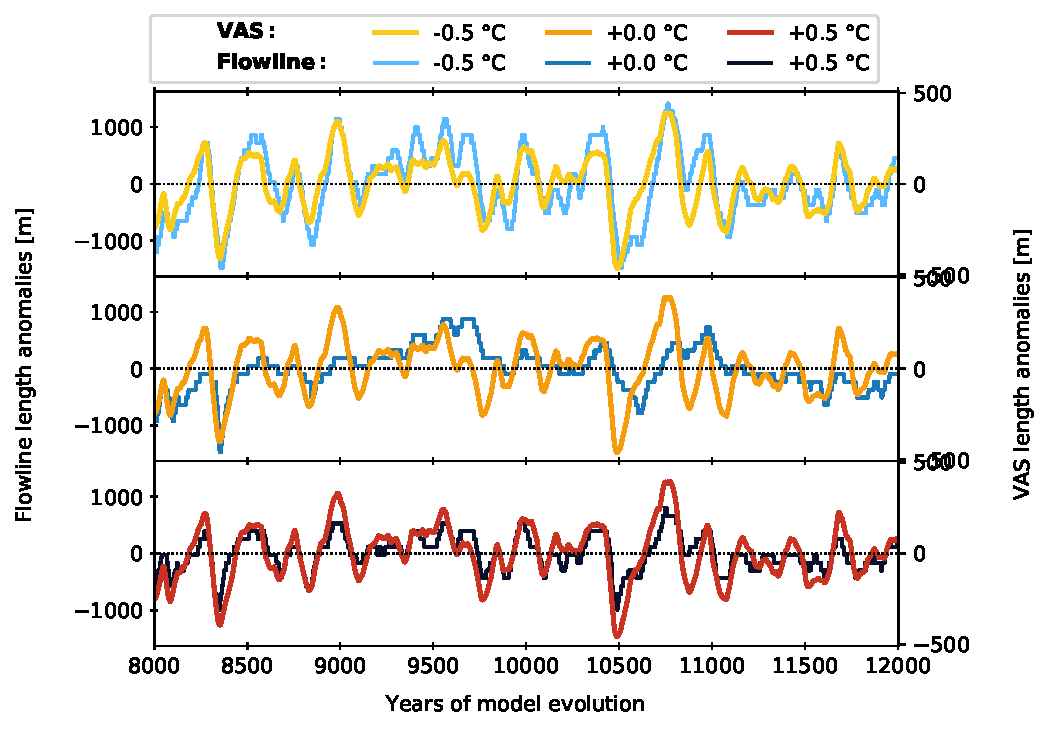
\includegraphics[width=\textwidth]{../plots/final_plots/random_length/Pasterze.pdf}
        \end{subfigure}
        \begin{subfigure}[b]{0.48\textwidth}
          \caption{RGI60-11.03643 - Mer de Glace}
          \label{fig:random_length:mer_de_glace}
          \centering
          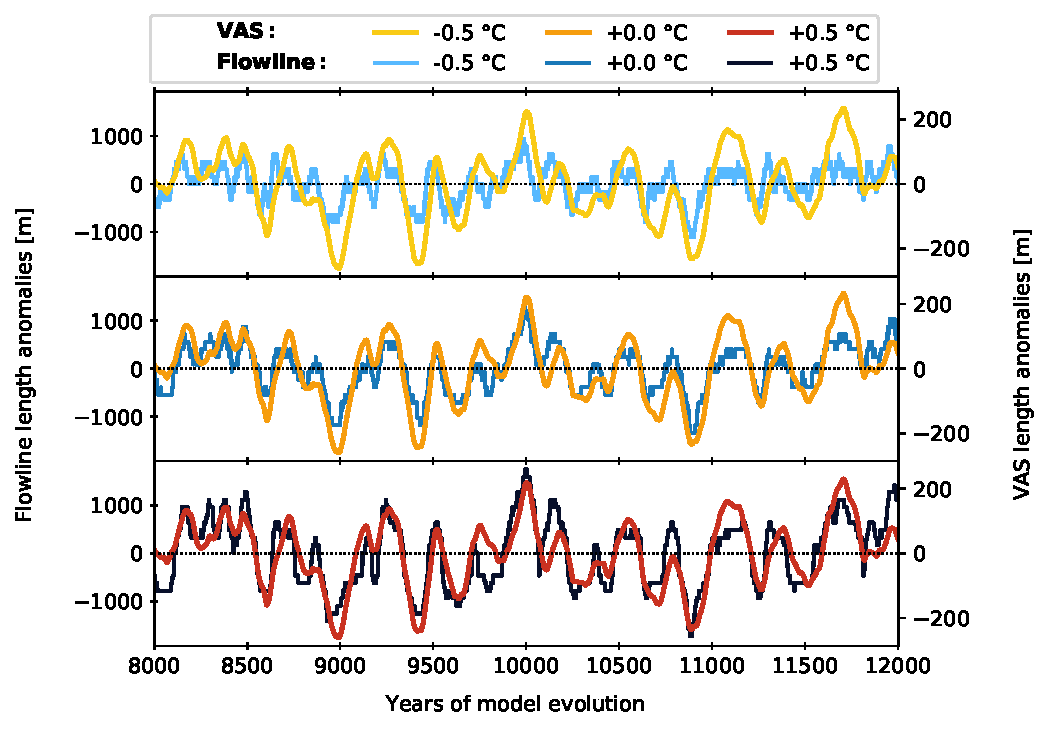
\includegraphics[width=\textwidth]{../plots/final_plots/random_length/Mer_de_Glace.pdf}
        \end{subfigure}
        \hfill
        \begin{subfigure}[b]{0.48\textwidth}
          \caption{RGI60-11.03638 - d'Argentière}
          \label{fig:random_length:glacier_d_argentiere}
          \centering
          \includegraphics[width=\textwidth]{../plots/final_plots/random_length/Glacier_d'Argentière.pdf}
        \end{subfigure}
        \begin{subfigure}[b]{0.48\textwidth}
          \caption{RGI60-11.01450 - Großer Aletschgletscher}
          \label{fig:random_length:großer_aletschgletscher}
          \centering
          \includegraphics[width=\textwidth]{../plots/final_plots/random_length/Großer_Aletschgletscher.pdf}
        \end{subfigure}
        \hfill
        \begin{subfigure}[b]{0.48\textwidth}
          \caption{RGI60-11.01238 - Rhonegletscher}
          \label{fig:random_length:rhonegletscher}
          \centering
          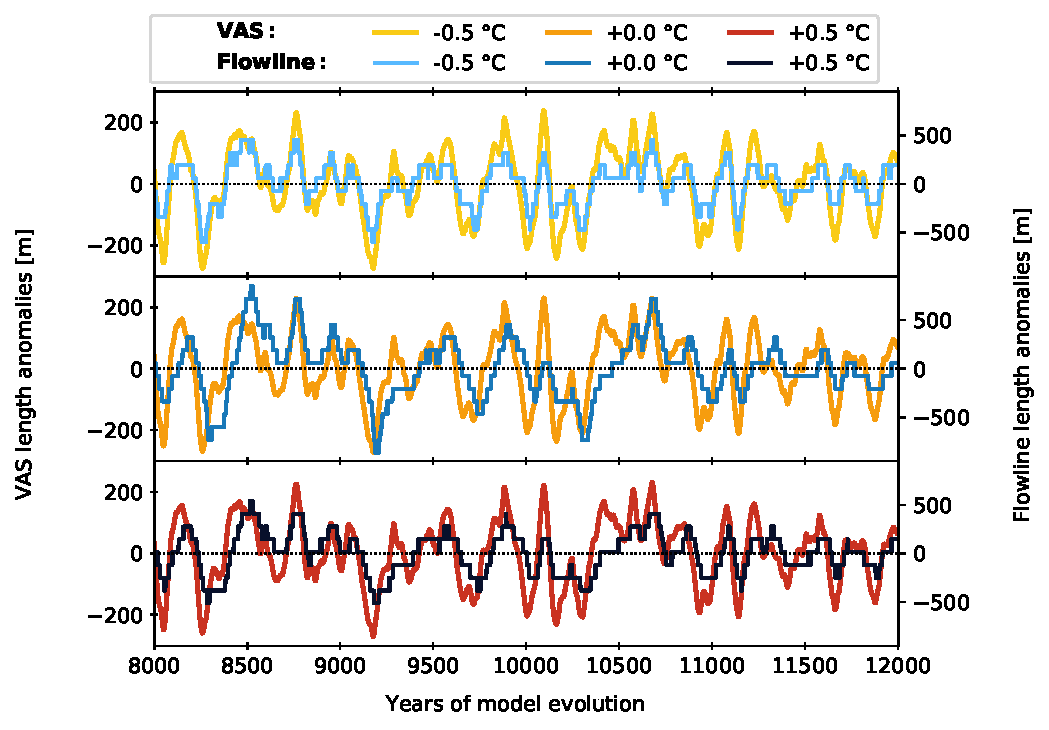
\includegraphics[width=\textwidth]{../plots/final_plots/random_length/Rhonegletscher.pdf}
        \end{subfigure}

        \caption{Length anomalies from to the respective average (equilibrium) value. The climate scenarios are based on a randomized equilibrium climate, with different temperature biases. Cyan, blue and purple lines represent the flowline model, while yellow, orange and red lines represent the \vas{} model, with a temperature bias of \SI{-.5}{\celsius}, \SI{0}{\celsius} and \SI{+.5}{\celsius}, respectively. Note the differences in y-axis scales.}
        \label{fig:random_length} 
      \end{figure}
      
      % PSD plots
      \begin{figure}[htp]
        \centering
        \begin{subfigure}[b]{0.48\textwidth}
          \caption{RGI60-11.00897 - Hintereisferner}
          \label{fig:psd:hintereisferner}
          \centering
          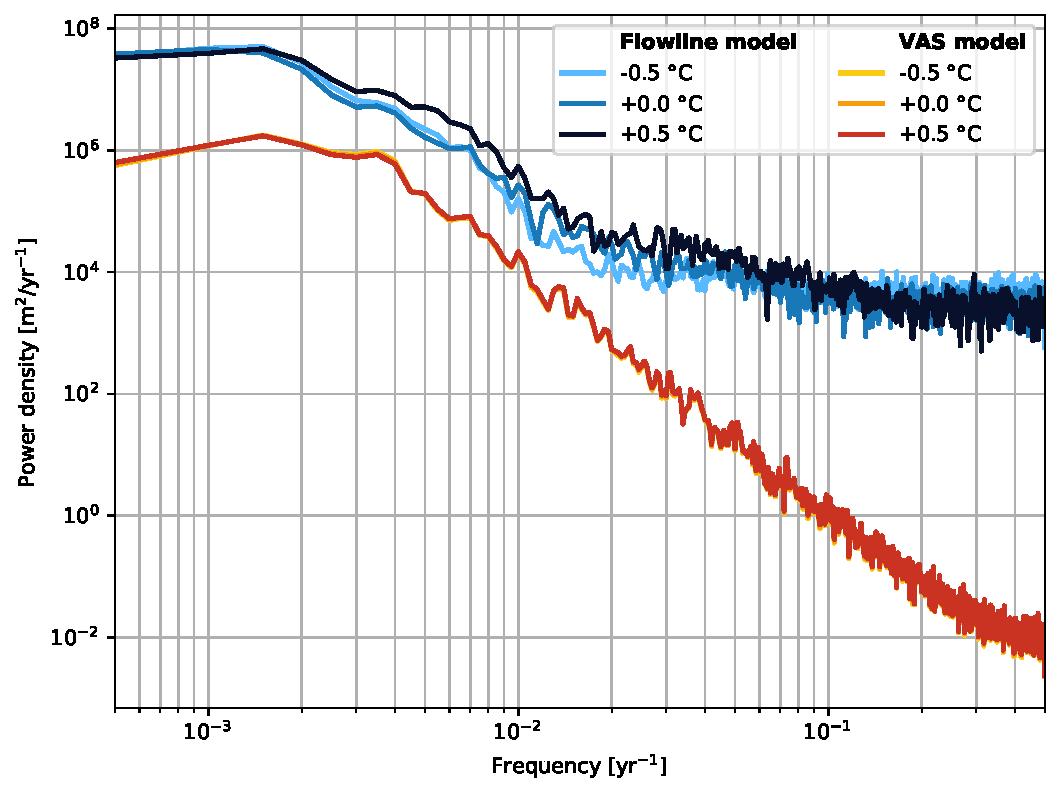
\includegraphics[width=\textwidth]{../plots/final_plots/psd/Hintereisferner.pdf}
        \end{subfigure}
        \hfill
        \begin{subfigure}[b]{0.48\textwidth}
          \caption{RGI60-11.00106 - Pasterze}
          \label{fig:psd:pasterze}
          \centering
          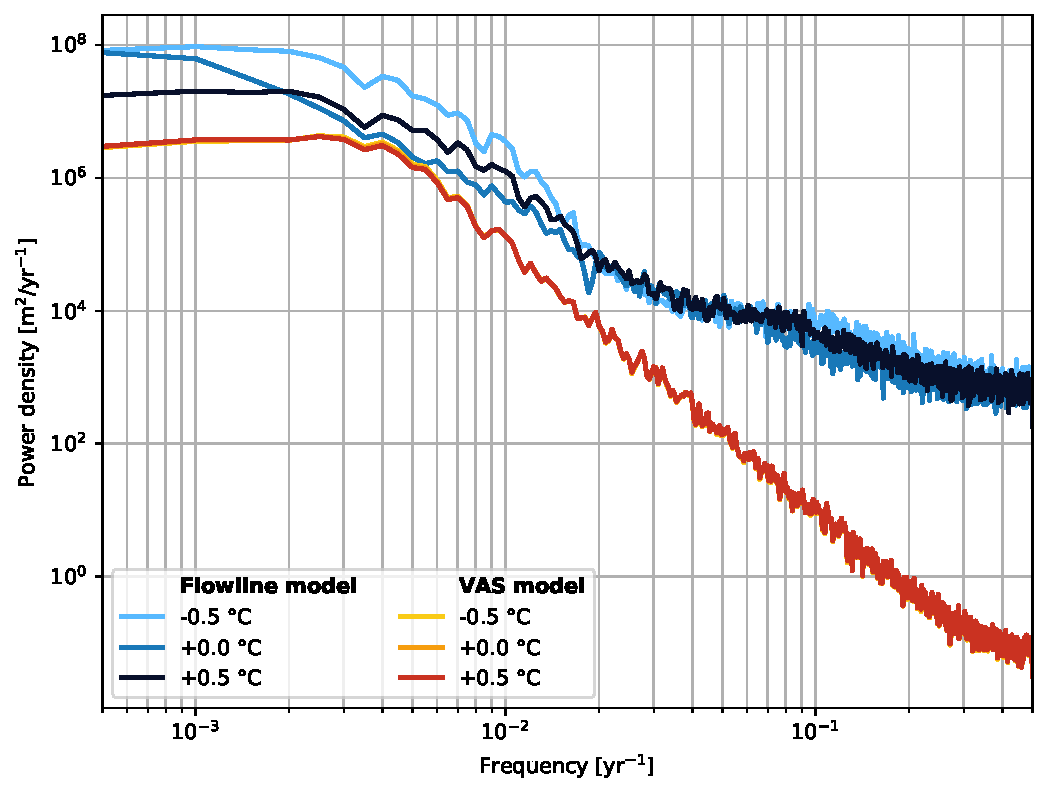
\includegraphics[width=\textwidth]{../plots/final_plots/psd/Pasterze.pdf}
        \end{subfigure}
        \begin{subfigure}[b]{0.48\textwidth}
          \caption{RGI60-11.03643 - Mer de Glace}
          \label{fig:psd:mer_de_glace}
          \centering
          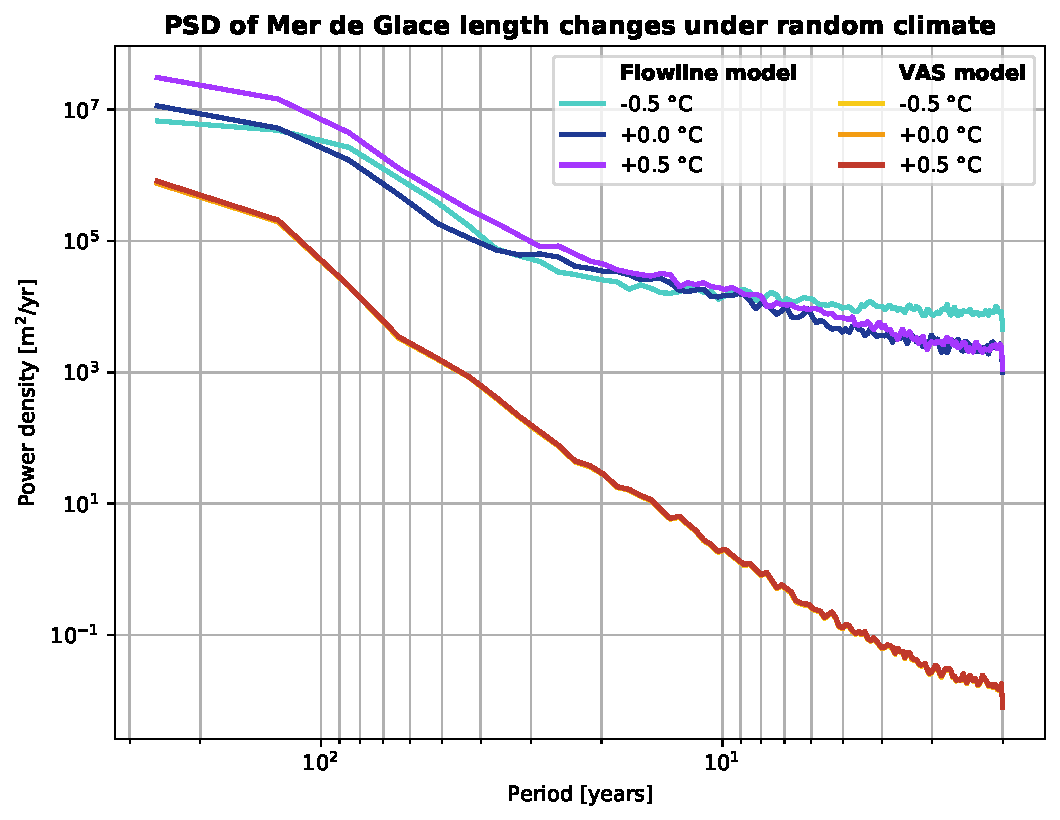
\includegraphics[width=\textwidth]{../plots/final_plots/psd/Mer_de_Glace.pdf}
        \end{subfigure}
        \hfill
        \begin{subfigure}[b]{0.48\textwidth}
          \caption{RGI60-11.03638 - d'Argentière}
          \label{fig:psd:glacier_d_argentiere}
          \centering
          \includegraphics[width=\textwidth]{../plots/final_plots/psd/Glacier_d'Argentière.pdf}
        \end{subfigure}
        \begin{subfigure}[b]{0.48\textwidth}
          \caption{RGI60-11.01450 - Großer Aletschgletscher}
          \label{fig:psd:großer_aletschgletscher}
          \centering
          \includegraphics[width=\textwidth]{../plots/final_plots/psd/Großer_Aletschgletscher.pdf}
        \end{subfigure}
        \hfill
        \begin{subfigure}[b]{0.48\textwidth}
          \caption{RGI60-11.01238 - Rhonegletscher}
          \label{fig:psd:rhonegletscher}
          \centering
          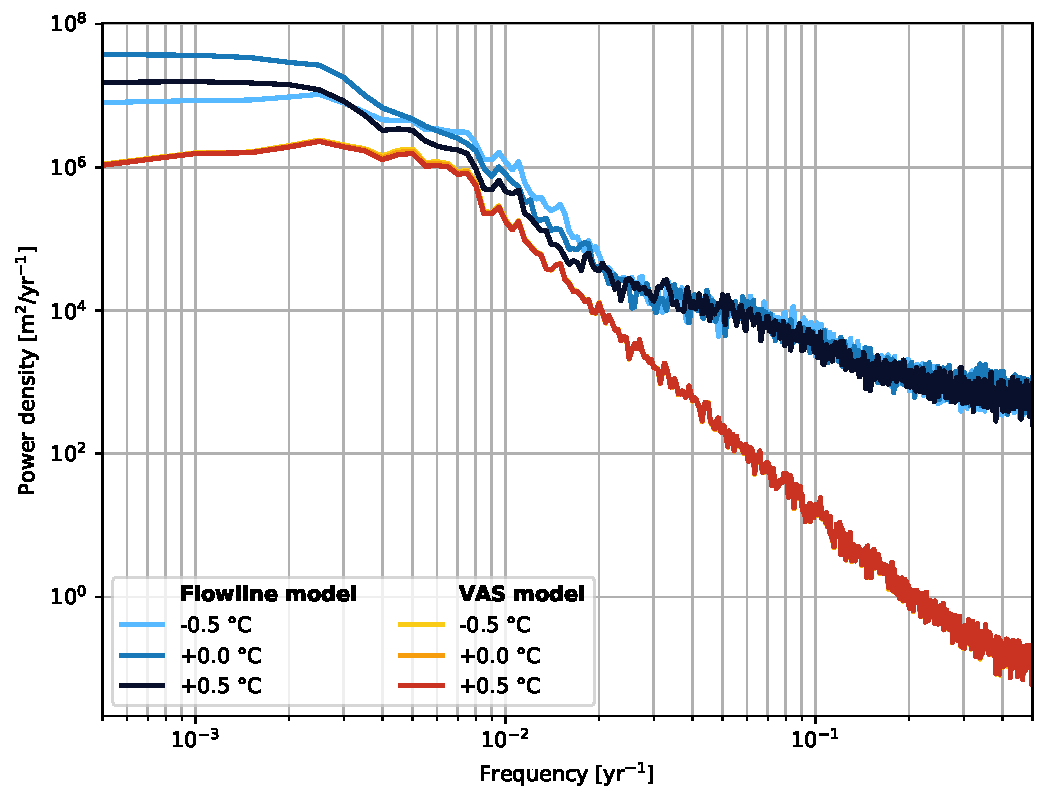
\includegraphics[width=\textwidth]{../plots/final_plots/psd/Rhonegletscher.pdf}
        \end{subfigure}

        \caption{Power spectral density of modeled glacier length for different alpine glaciers. Different lines represent different combinations of evolution models and climate scenarios. The climate scenarios are based on a randomized equilibrium climate, with different temperature biases. Cyan, blue and purple lines represent the flowline model, while yellow, orange and red lines represent the \vas{} model, with a temperature bias of \SI{-.5}{\celsius}, \SI{0}{\celsius} and \SI{+.5}{\celsius}, respectively. Note the differences in y-axis scales.}
        \label{fig:psd}
      \end{figure}
    
    % subsection power_spectral_density_results (end)

    \subsection{Autocorrelation function} % (fold)
    \label{sub:autocorrelation_function_results}

      A general observation about the ACF can be made for both models, all glaciers and climate scenarios: the correlation is high for the first few lag times, before it decreases exponentially. This points at an autoregressive (AR) term and a moving-average (MA) term in the data. An autoregressive-moving-average model (ARMA) predicts future values of a random variable based on a linear combination of the past values and past error terms of said variable. This makes intuitive sense for glaciers, since the past and current glacier size and the difference to the equilibrium value have a direct influence on next years glacier size. A more detailed discussion of a potential ARMA model is provided at the end of this section.

      Same as for the PSDs, the ACFs for the \vas{} length signals are almost identical between different sizes of the same glacier, indicating that the glacier size has little to no effect on the transient behavior of the model. The \vas{} model represents the glacier as a simple cuboid without any additional information about the glacier shape. The absolute dimensions of that cuboid seem to have less of an effect on the ACF than other parameters, which differe from glacier to glacier. Some glaciers, like the Glacier d'Argentière and the Aletschgletscher show statistically significant negative correlations for higher lag terms between 80 and 250 years, while the others show very little to no significant negative correlation for higher lag times. However, no apparent relation between the strength of negative correlations for later lag times and any other glacier parameter, like the average slope or the model-internal lag times, was found.
      The average slope is the only additional geometric information of the \vas{} model, even if it is implemented only indirectly. The slope is independent of the glacier's sizes. However, it affects the temporal evolution, since changes in terminus elevation---and thereby changes in specific mass balance---are linearly related to changes in glacier length. This can be seen in the ACF plots, which vary from glacier to glacier but not between different sizes of the same glacier.  However, their is no obvious pattern when comparing the ACF to the average slope\footnote{Possible future work could include a in-depth investigation on how glacier characteristics influence its ACF. Thereby, the ACF could add information, or even superseed, to the concept of e-folding response times as glacier characteristics.}.
    
      The flowline model is able to represent different glacier geometries and grasp individual responses under different equilibrium climates, which can be seen in the vastly different ACFs. They differ from glacier to glacier, but also for different sizes of the same glacier. However, there are again no discernible patterns, which confirms the notion that the flowline model is capable of simulating each glacier's individual response. The autocorrelation of the flowline model is generally stronger than for the \vas{} runs for most glaciers and most temperature biases, even though not for all. The following list points to some particular observations:
      \begin{itemize}
        \item for Hintereisferner (Figure~\ref{fig:acf:hintereisferner}) the ACFs of the flowline model show higher correlations than for the \vas{} model, while for Mer de Glace (Figure~\ref{fig:acf:mer_de_glace}) and Großer Aletschgletscher (Figure~\ref{fig:acf:großer_aletschgletscher}) the flowline model ACFs show equal ore lower correlations for lag time up to around fifty years;
        \item the flowline model of the Pasterze (Figure~\ref{fig:acf:pasterze}) shows a strong autocorrelation under the equilibrium climate, i.e., for its medium size, ($r>0.6$ for lags times up to one-hundred years and statistically significant up until a lag time of 243 years), while under a warmer and colder equilibrium climate (\SI{\pm0.5}{\celsius}) the autocorrelation of all lag times is comparable to the \vas{} model;
        \item similarly, the flowline model of the Glacier d'Argentière (Figure~\ref{fig:acf:glacier_d_argentiere}) shows a strong autocorrelation under the warmer equilibrium climate (\SI{+0.5}{\celsius}), while the autocorrelation under the other two climate scenarios is even lower than the ACF of the \vas{} model.
      \end{itemize}
      The only observation made for all glaciers, it that the \vas{} model shows a stronger or equal autocorrelation for shorter lag time (i.e., less than about twenty years) than the flowline model. This is true even for glaciers, where the autocorrelation of the flowline mode is generally stronger than for the \vas{} model (e.g., Hintereisferner).

      Strong correlations for short lag times influences the correlation of all following lag terms. For example, an exponentially decaying signal, which halves its value with each time step $\Phi(t) = 0.5 \Phi(t-1)$, will have an autocorrelation of 0.5 for lag 1, 0.25 for lag 2, 0.125 for lag 3, and so on. Depending on the sample size these values will be statistically significant, even though only one lag term is included in the definition of the signal (i.e., an AR(1) process). The partial autocorrelation function (PACF) measures only these direct influences, eliminating the effects of all shorter lag times. All the PACFs of the \vas{} model lengths show a strong positive correlation for lag times of 1 year, followed by a strong negative correlation which then slowly increases towards zero. Correlations for lag times ten and greater are not, or only marginally, significant. Again, there are no discernible differences between different sizes of the same glacier and very little differences from one glacier to another. The PACFs for the flowline model lengths show the same high correlation for the lag time of one year, before decreasing towards zero. The decrease towards statistical insignificant correlations happens quite fast for most glaciers. Only Mer de Glace (Figure~\ref{fig:pacf:mer_de_glace}) and Glacier d'Argentière (Figure~\ref{fig:pacf:glacier_d_argentiere}), both for the warmer climate, and Rhonegletscher (Figure~\ref{fig:pacf:rhonegletscher}), for the equilibrium climate, show significant correlations for lag times greater than three years. For higher lag times between ten and twenty years there are some negative correlations, even though they are only marginally significant.

      The number of statistically significant terms of the PACF informs on the order $p$ for the AR($p$) model. The order specifies the of number lag terms that are considered. Analogously, the order $q$ for the MA($q$) model can be estimated from the number of significant terms of the ACF. By this definition, the \vas{} model could be ... by an ARMA(9, 70) model, and the flowline model by an ARMA(3, 140). Hereby, the orders are taken as average over all glaciers and climate scenarios (see Appendix~\ref{appendix_B} for details). While an AR model with nine lag terms would be big but still feasible, a MA model with over one-hundred lag terms is neither practicable nor does it make sense. Especially, since \citet{Roe2014} use an ARMA(3,3) model to produce comparable results to a flowline model. It is not the intent of this work to investigate the relation between a glacier's geometry and its ACF, neither to fit an ARMA model to the data. Hence, this qualitative first look has to suffice. However, it is most notable that the flowline model behaves differently not only for different glaciers, but also for different sizes of the same glacier. The \textit{one size fits all} approach of the \vas{} model produces more homogeneous results, the ACFs and PACFs are mostly independent of a glacier's size.

      \begin{figure}[htp]
        \centering
        
        \begin{subfigure}[b]{0.48\textwidth}
          \caption{RGI60-11.00897 - Hintereisferner}
          \label{fig:acf:hintereisferner}
          \centering
          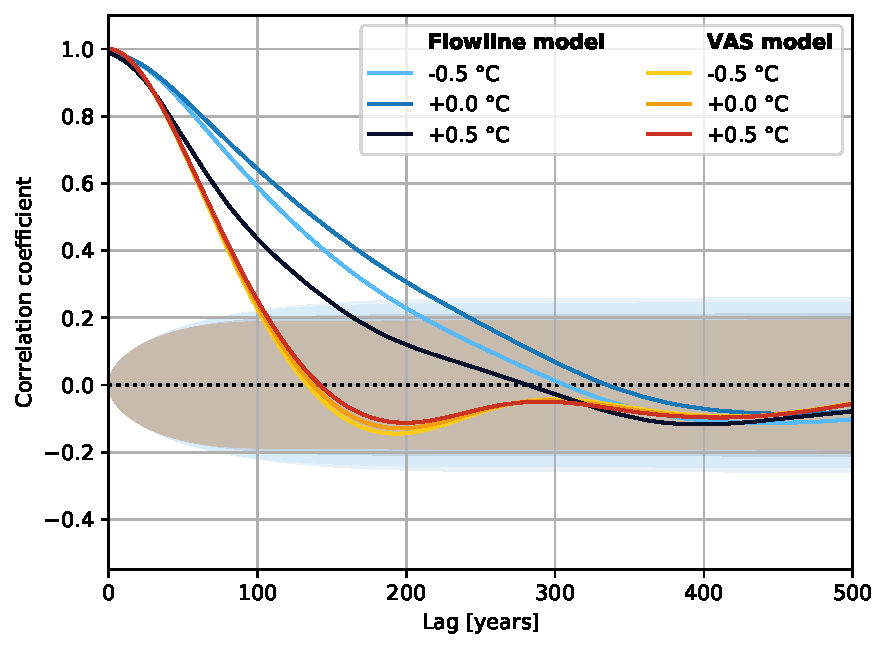
\includegraphics[width=\textwidth]{../plots/final_plots/acf/Hintereisferner.pdf}
        \end{subfigure}
        \hfill
        \begin{subfigure}[b]{0.48\textwidth}
          \caption{RGI60-11.00106 - Pasterze}
          \label{fig:acf:pasterze}
          \centering
          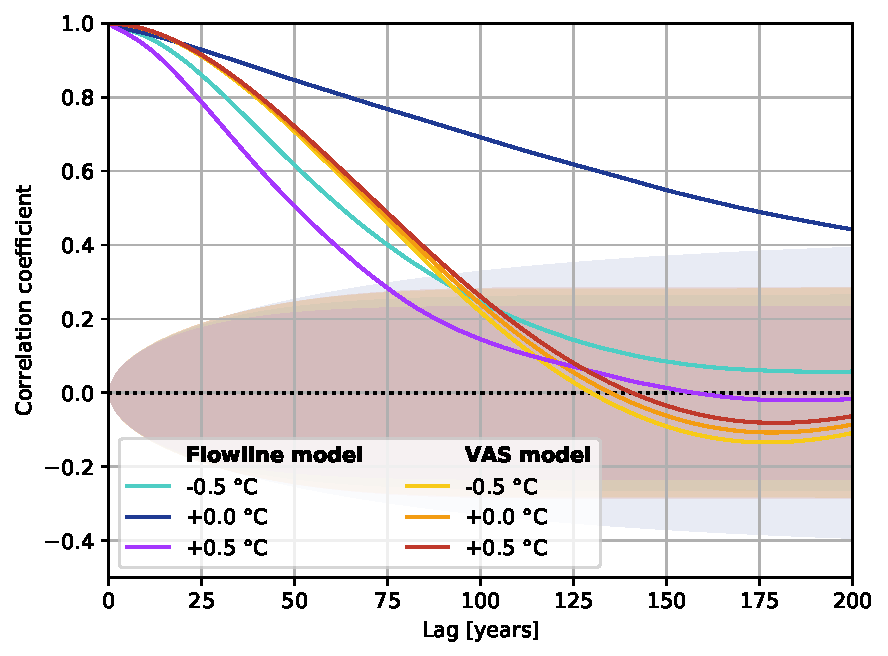
\includegraphics[width=\textwidth]{../plots/final_plots/acf/Pasterze.pdf}
        \end{subfigure}

        \begin{subfigure}[b]{0.48\textwidth}
          \caption{RGI60-11.03643 - Mer de Glace}
          \label{fig:acf:mer_de_glace}
          \centering
          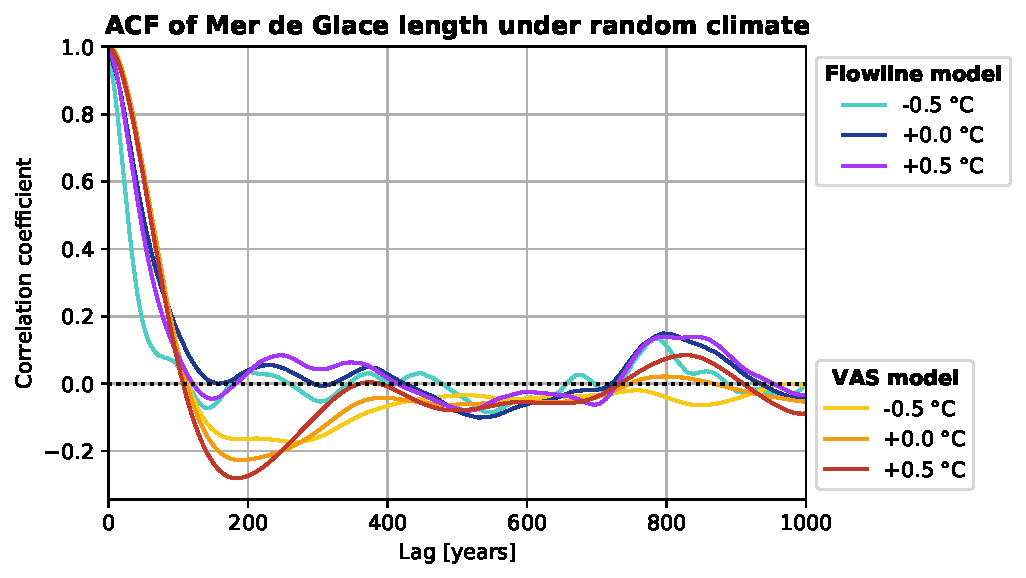
\includegraphics[width=\textwidth]{../plots/final_plots/acf/Mer_de_Glace.pdf}
        \end{subfigure}
        \hfill
        \begin{subfigure}[b]{0.48\textwidth}
          \caption{RGI60-11.03638 - d'Argentière}
          \label{fig:acf:glacier_d_argentiere}
          \centering
          \includegraphics[width=\textwidth]{../plots/final_plots/acf/Glacier_d'Argentière.pdf}
        \end{subfigure}

        \begin{subfigure}[b]{0.48\textwidth}
          \caption{RGI60-11.01450 - Großer Aletschgletscher}
          \label{fig:acf:großer_aletschgletscher}
          \centering
          \includegraphics[width=\textwidth]{../plots/final_plots/acf/Großer_Aletschgletscher.pdf}
        \end{subfigure}
        \hfill
        \begin{subfigure}[b]{0.48\textwidth}
          \caption{RGI60-11.01238 - Rhonegletscher}
          \label{fig:acf:rhonegletscher}
          \centering
          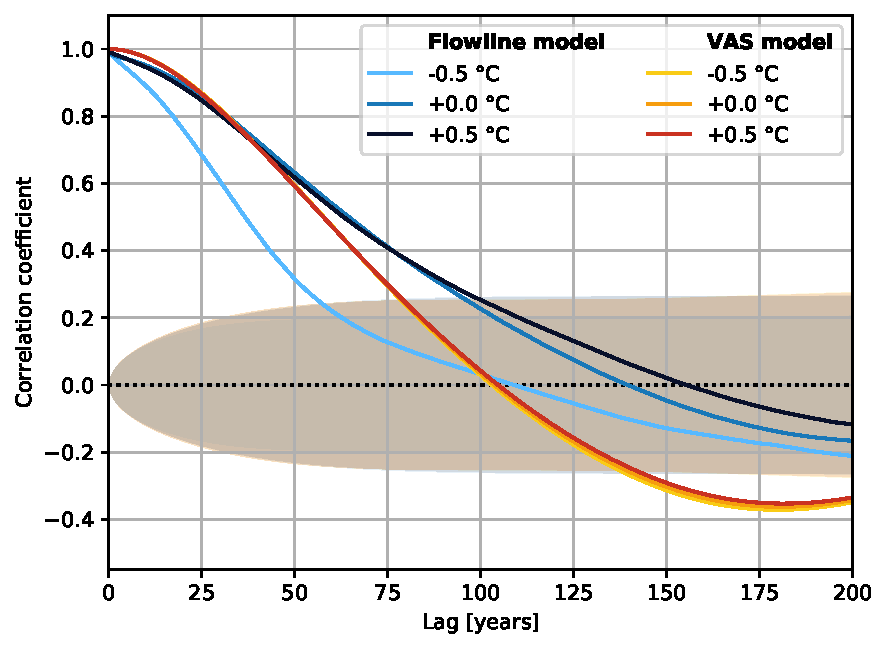
\includegraphics[width=\textwidth]{../plots/final_plots/acf/Rhonegletscher.pdf}
        \end{subfigure}

        \caption{Autocorrelation function of modeled length for lag times between zero and 200 years. Different lines represent different combinations of evolution model and climate scenario.
        The random climate scenario is based on an equilibrium climate, with different temperature biases.
        Cyan, blue and purple lines represent the flowline model, while yellow, orange and red lines represent the \vas{} model, with a temperature bias of \SI{-.5}{\celsius}, \SI{0}{\celsius} and \SI{+.5}{\celsius}, respectively.
        The \SI{99}{\percent} confidence intervals are shaded in the corresponding colors.}
        \label{fig:acf}
      \end{figure}

      \begin{figure}[htp]
        \centering
        
        \begin{subfigure}[b]{0.48\textwidth}
          \caption{RGI60-11.00897 - Hintereisferner}
          \label{fig:pacf:hintereisferner}
          \centering
          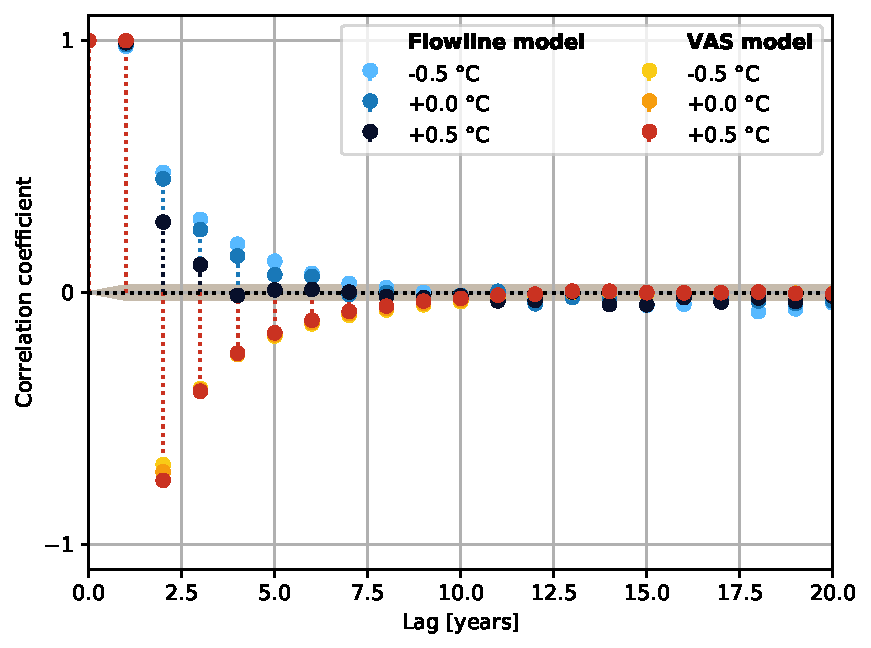
\includegraphics[width=\textwidth]{../plots/final_plots/pacf/Hintereisferner.pdf}
        \end{subfigure}
        \hfill
        \begin{subfigure}[b]{0.48\textwidth}
          \caption{RGI60-11.00106 - Pasterze}
          \label{fig:pacf:pasterze}
          \centering
          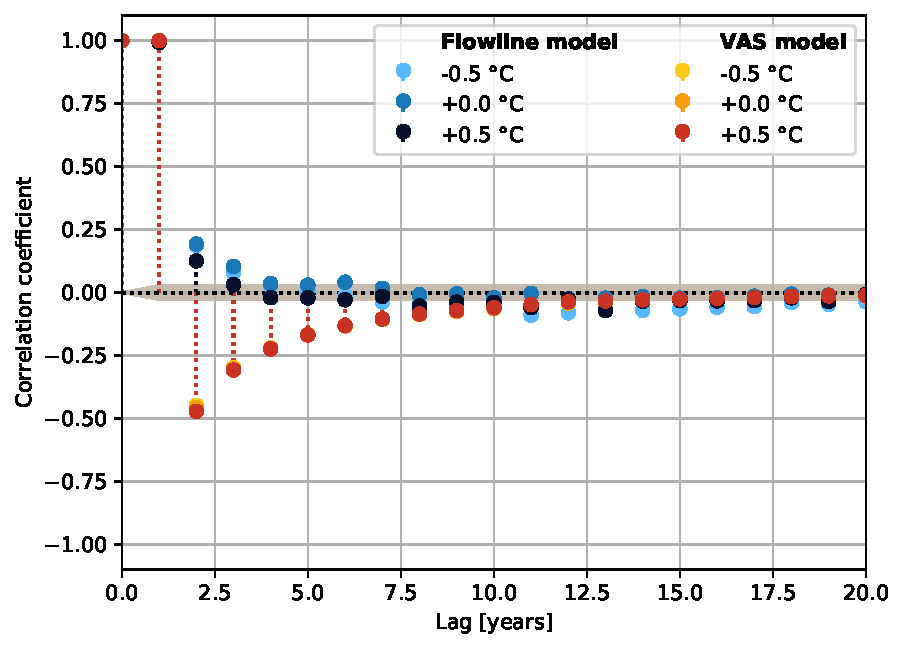
\includegraphics[width=\textwidth]{../plots/final_plots/pacf/Pasterze.pdf}
        \end{subfigure}

        \begin{subfigure}[b]{0.48\textwidth}
          \caption{RGI60-11.03643 - Mer de Glace}
          \label{fig:pacf:mer_de_glace}
          \centering
          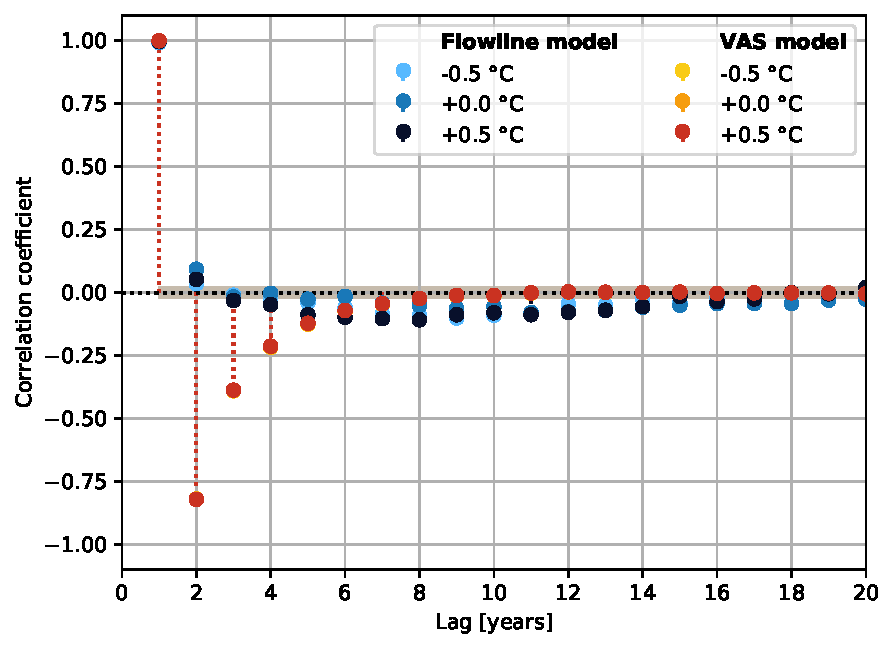
\includegraphics[width=\textwidth]{../plots/final_plots/pacf/Mer_de_Glace.pdf}
        \end{subfigure}
        \hfill
        \begin{subfigure}[b]{0.48\textwidth}
          \caption{RGI60-11.03638 - d'Argentière}
          \label{fig:pacf:glacier_d_argentiere}
          \centering
          \includegraphics[width=\textwidth]{../plots/final_plots/pacf/Glacier_d'Argentière.pdf}
        \end{subfigure}

        \begin{subfigure}[b]{0.48\textwidth}
          \caption{RGI60-11.01450 - Großer Aletschgletscher}
          \label{fig:pacf:großer_aletschgletscher}
          \centering
          \includegraphics[width=\textwidth]{../plots/final_plots/pacf/Großer_Aletschgletscher.pdf}
        \end{subfigure}
        \hfill
        \begin{subfigure}[b]{0.48\textwidth}
          \caption{RGI60-11.01238 - Rhonegletscher}
          \label{fig:pacf:rhonegletscher}
          \centering
          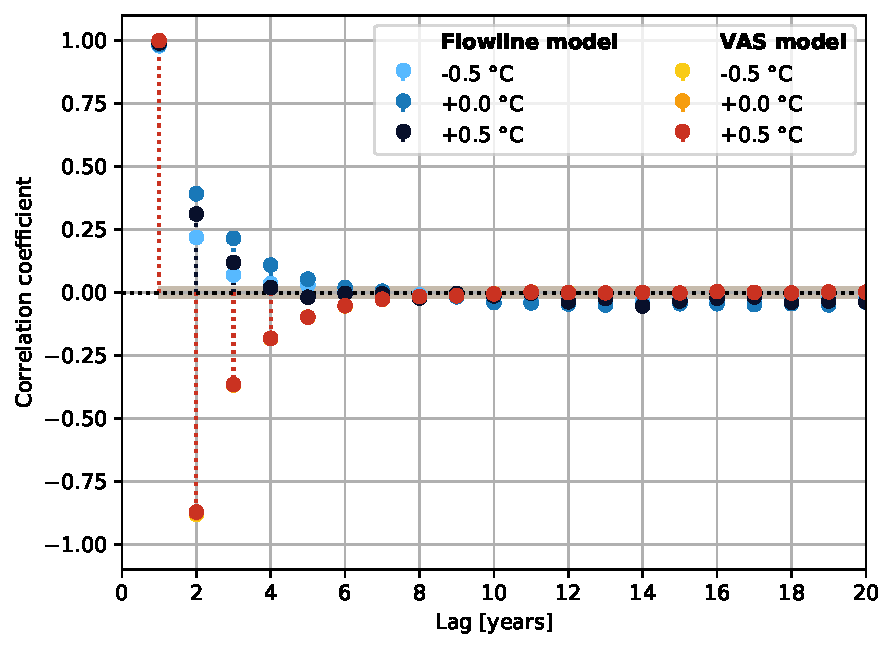
\includegraphics[width=\textwidth]{../plots/final_plots/pacf/Rhonegletscher.pdf}
        \end{subfigure}

        \caption{Partial autocorrelation function of modeled length for lag times between zero and 200 years. Different lines represent different combinations of evolution model and climate scenario.
        The random climate scenario is based on an equilibrium climate, with different temperature biases.
        Cyan, blue and purple lines represent the flowline model, while yellow, orange and red lines represent the \vas{} model, with a temperature bias of \SI{-.5}{\celsius}, \SI{0}{\celsius} and \SI{+.5}{\celsius}, respectively.
        The \SI{99}{\percent} confidence intervals are shaded in the corresponding colors.}
        \label{fig:pacf}
      \end{figure}

    % subsection autocorrelation_function_results (end)

  % section autocorrelation_fand_power_spectral_density_results (end)

  \section{Regional runs with all Alpine glaciers} % (fold)
  \label{sec:regional_runs_with_all_alpine_glaciers_results}

    \Vas{} should not be applied to individual glaciers, but only to populations of glaciers \citep{Bahr2015}, where the scaling approach shows its strength: the law of large number assures a reasonable estimation of the collective glacier ice volume, since random errors will be canceled out by each other. This section compares the behavior of the \vas{} model to the flowline model, on the example of all Alpine glaciers under different climate scenarios (analogous to the single glacier test case, see Section~\ref{sec:single_glacier_test_case_results}).
    Again, both mass balance models simulate different climate scenarios with the same three temperature biases as above, based on the equilibrium period centered around \lstinline`y0` = \tstar{}. The only difference to the single glacier test case is that the \vas{} model and the flowline model each use their respective \tstar{} reference tables. For more details about the experimental setup see Section~\ref{sub:regional_runs_with_all_alpine_glaciers_setup}. The time series plots of normalized and absolute total Alpine ice volume are shown in Figure~\ref{fig:histalp_commitment}.

    Both evolution models run for 1000 years with the \lstinline`ConstantMassBalance` model and the \lstinline`RandomMassBalance` model. The random climate with its year-to-year fluctuations is obviously more physical than the completely constant climate. However, the resulting changes in glacier ice volume under both climate scenarios are almost identical. This makes intuitive sense, considering that glaciers act as natural low-pass filters for climatic variabilities (as established above, see Section~\ref{sub:power_spectral_density_results}). Short term climatic variabilities have little to no effect on the ice volume of a single glacier, much less on the aggregate ice volume of an entire region. Over the last 200 years of the simulations, the relative differences in aggregate ice volume between the constant and random climate scenario never exceed \SI{0.6}{\percent} for the \vas{} model and \SI{1.7}{\percent} for the flowline model. Only the \SI{0}{\celsius}-run of flowline model shows higher relative differences, with an average of \SI{2.0}{\percent} over the last 200 years, up to a maximum of \SI{2.7}{\percent}. While the total ice volume stays close to it's initial value, it shows a slight increase over time. After an initially strong increase of \SI{1.6}{\percent} over the first fifty years and another fifty years of constant values, the volume grows almost linearly with about \SI{0.53}{\cubic\kilo\meter} per 100 years under the constant climate scenario. This results in a total volume change of \SI{5.6}{\cubic\kilo\meter} (\SI{+3.4}{\percent} of the initial value) after 1000 years of simulation. Under the random climate scenario, the total ice volume grows slower, most likely since the oscillations will reduce certain feedback loops. Long story short, the following discussion is simplified by only considering the constant climate scenarios. 

    The \vas{} model estimates a total Alpine ice volume of \SI{156}{\cubic\kilo\meter} (\SI{+20}{\percent}), \SI{130}{\cubic\kilo\meter} (\SI{\pm{}0}{\percent}) and \SI{109}{\cubic\kilo\meter} (\SI{-17}{\percent}), while the flowline model estimates a total Alpine ice volume of \SI{259}{\cubic\kilo\meter} (\SI{+59}{\percent}), \SI{169}{\cubic\kilo\meter} (\SI{+3}{\percent}) and \SI{92}{\cubic\kilo\meter} (\SI{-44}{\percent}), after 1000 years of simulation under a temperature bias of \SI{-0.5}{\celsius}, \SI{0}{\celsius} and \SI{+0.5}{\celsius}, respectively.

    All the general characteristics of the \vas{} model found for the Hintereisferner test case turn up again for the regional. The \vas{} scaling model underestimates the changes in ice volume compared to the flowline model by a factor of \num{\approx 3.5}. The oscillatory behavior of the \vas{} model is still visible The \vas{} model's response time scales to the step changes in climate are shorter that for the flowline model. The volume e-folding time scales of both models are comparable to the single glacier test case: $\tau_V = \SI{23}{\year}$ and $\tau_V = \SI{20}{\year}$ for the \vas{} model and $\tau_V = \SI{125}{\year}$ and $\tau_V = \SI{79}{\year}$ for the flowline model, for the negative and positive temperature perturbation, respectively. These values are highly influenced by the larger glaciers and serve only as a guidance level. The symmetric behavior of the \vas{} model is still reflected in the response times, but less so in the new equilibrium values.

    All in all, the \vas{} model does a bad job compared to the flowline model, even though no statement about the model accuracy can be made without any comparison to observational data. The next section explores the possibilities of tuning the \vas{} model via different parameters for the used scaling relations. This also provides a range of plausible results and serves as uncertainty estimation.

    \begin{figure}[htp]
      \centering
      \begin{subfigure}[b]{0.48\textwidth}
        \caption{\Vas{} model, relative glacier volume}
        \label{fig:histalp_commitment:volume_norm_const}
        \centering
        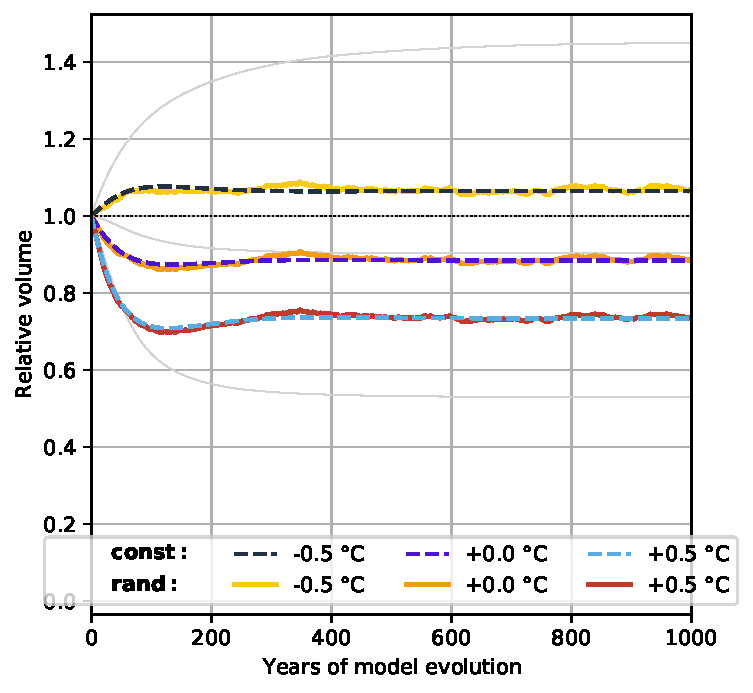
\includegraphics[width=\textwidth]{../plots/final_plots/time_series/histalp_commitment/volume_norm_vas.pdf}
      \end{subfigure}
      \hfill
      \begin{subfigure}[b]{0.48\textwidth}
        \caption{Flowline model, relative glacier volume}
        \label{fig:histalp_commitment:volume_norm_random}
        \centering
        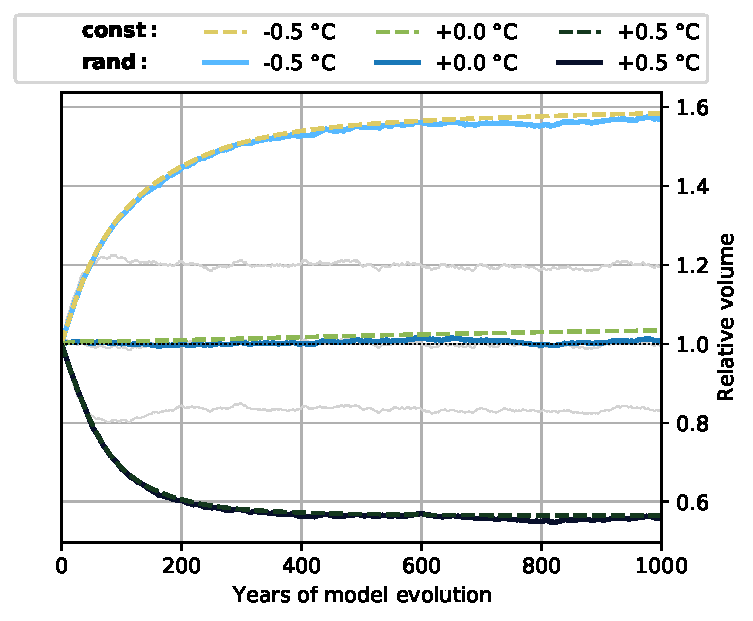
\includegraphics[width=\textwidth]{../plots/final_plots/time_series/histalp_commitment/volume_norm_fl.pdf}
      \end{subfigure}
      \begin{subfigure}[b]{0.48\textwidth}
        \caption{\Vas{} model, absolute glacier volume}
        \label{fig:histalp_commitment:volume_abs_const}
        \centering
        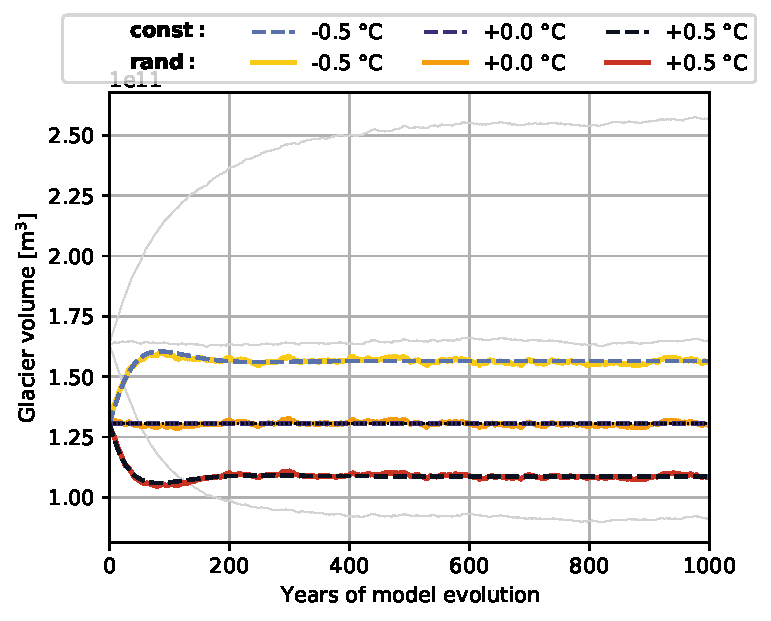
\includegraphics[width=\textwidth]{../plots/final_plots/time_series/histalp_commitment/volume_abs_vas.pdf}
      \end{subfigure}
      \hfill
      \begin{subfigure}[b]{0.48\textwidth}
        \caption{Flowline model, absolute glacier volume}
        \label{fig:histalp_commitment:volume_abs_random}
        \centering
        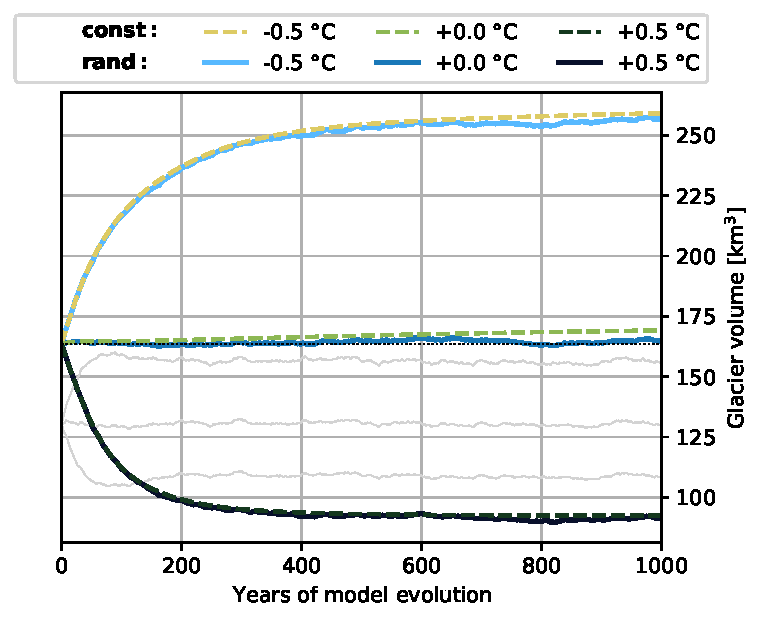
\includegraphics[width=\textwidth]{../plots/final_plots/time_series/histalp_commitment/volume_abs_fl.pdf}
      \end{subfigure}
      
      \caption{Time series of total ice volume for all glaciers in the HISTALP domain. The upper two panels show the relative glacier ice volume, normalized with the initial values, while the lower two panels show the absolute glacier ice volume. The left panels show the result of the \vas{} model, the right panels show the results of the flowline model. Solid lines represent the random climate scenarios, while dashed lines represent the constant climate scenarios. All climate scenarios are based on an equilibrium climate, with one of three different temperature biases.
      Yellow, orange and red solid lines represent the \vas{} model, while cyan, blue and purple solid lines represent the flowline model, under a random climate with a temperature bias of \SI{-.5}{\celsius}, \SI{0}{\celsius} and \SI{+.5}{\celsius}, respectively. Yellow, orange and red dashed lines represent the \vas{} model, while cyan, blue and purple dashed lines represent the flowline model, under a constant climate with a temperature bias of \SI{-.5}{\celsius}, \SI{0}{\celsius} and \SI{+.5}{\celsius}, respectively. %TODO change colors
      The dotted line indicate the initial volume. The light gray lines represent the volume evolutions of the other model, to facilitate comparisons.}
      \label{fig:histalp_commitment}
    \end{figure}

  % section regional_runs_with_all_alpine_glaciers_results (end)

  \section{Sensitivity experiments} % (fold)
  \label{sec:sensitivity_experiments_results}

    All the experiments performed above show quite large differences in projected ice volume change between the \vas{} model and the flowline model. However, the ``out-of-the-box'' scaling model is maybe not the best fit for the Alpine glaciers, and it is definitely not a good fit for any single glacier. Hence, tuning a set of parameters may improve the model performance.
    The most obvious tuning parameters are the model-internal time scales, and the scaling constants and scaling exponents. The following sensitivity experiments run the \vas{} model with different values for these parameters. As before, the experiments are performed on the Hintereisferner (RGI60-11.00897) and on all Alpine glaciers in the HISTALP domain, in each case with a constant equilibrium climate scenario and a positive temperature bias of \SI{+0.5}{\celsius}. For details about the experimental setup see Section~\ref{sub:sensitivity_experiments_setup}.

    \begin{tldrbox}[Sensitivity experiments]{tldr:sensitivity_experiments_results}
      \item The model-internal time scales control the damping ratio of the oscillation, longer time scales correspond to stronger overshoots.
      \item Halving the model-internal time scales leads to an almost asymptotic change in aggregate ice volume of the HISTALP domain, showing only negligible oscillations.
      \item Different scaling constants lead to a different initial ice volume and a different initial glacier length, which in turn affect the e-folding time scales.
      \item Changing the scaling constants has little to no effect on the normalized volume change and normalized equilibrium volume.
      \item Custom scaling constants and exponents increase the change in ice volume ever so slightly, but the results are still not comparable to the flowline model.
    \end{tldrbox}
    
    \begin{figure}[ht]
      \centering
      % HEF time scales
      \begin{subfigure}[b]{0.476\textwidth}
        \caption{Hintereisferner, different model-internal time scales}
        \label{fig:sensitivity:time_scales_hef}
        \centering
        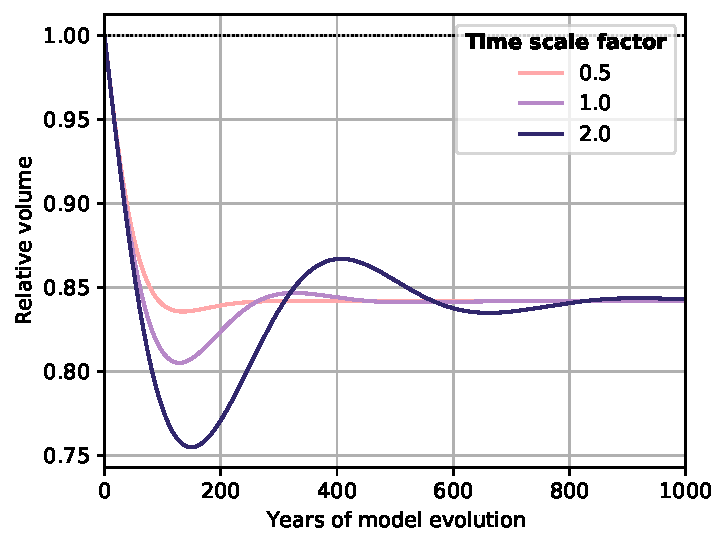
\includegraphics[width=\textwidth]{../plots/final_plots/sensitivity/time_scales_hef.pdf}
      \end{subfigure}
      \hfill
      % HEF scaling params
      \begin{subfigure}[b]{0.476\textwidth}
        \caption{Hintereisferner, different scaling constants}
        \label{fig:sensitivity:scaling_params_hef}
        \centering
        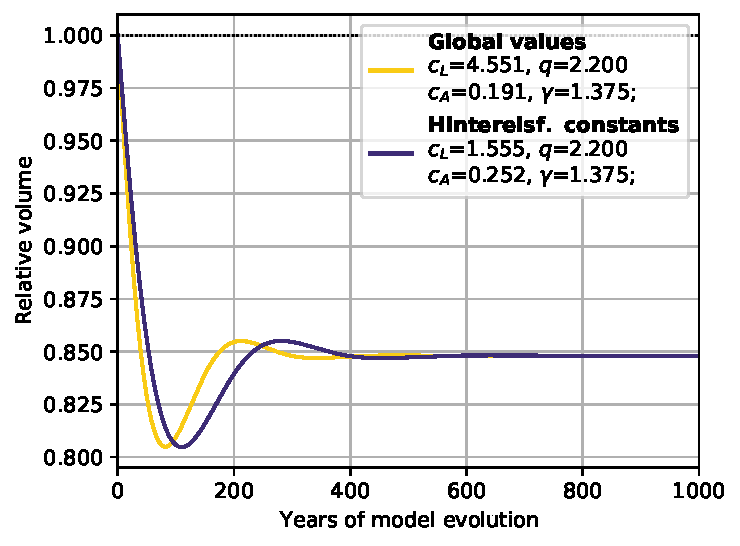
\includegraphics[width=\textwidth]{../plots/final_plots/sensitivity/scaling_params_hef.pdf}
      \end{subfigure}
      
      % HISTALP time scales
      \begin{subfigure}[b]{0.476\textwidth}
        \caption{HISTALP domain, different model-internal time scales}
        \label{fig:sensitivity:time_scales_histalp}
        \centering
        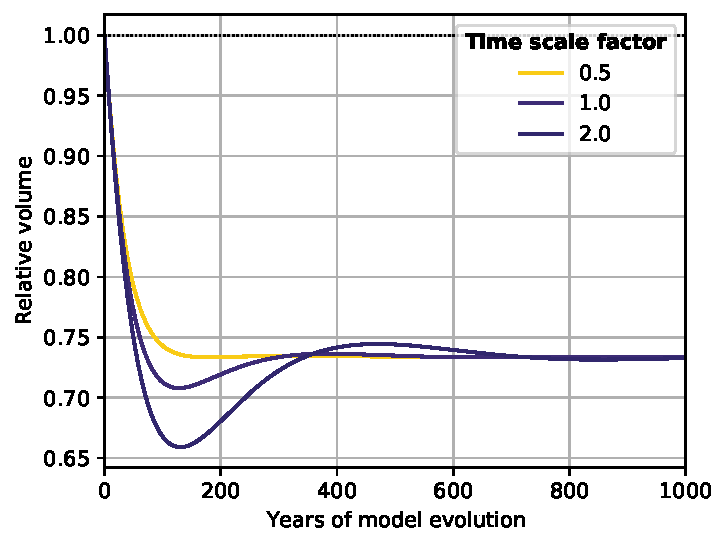
\includegraphics[width=\textwidth]{../plots/final_plots/sensitivity/time_scales_histalp.pdf}
      \end{subfigure}
      \hfill
      % HISTALP scaling params
      \begin{subfigure}[b]{0.476\textwidth}
        \caption{HISTALP domain, different scaling constants and scaling exponents}
        \label{fig:sensitivity:scaling_params_histalp}
        \centering
        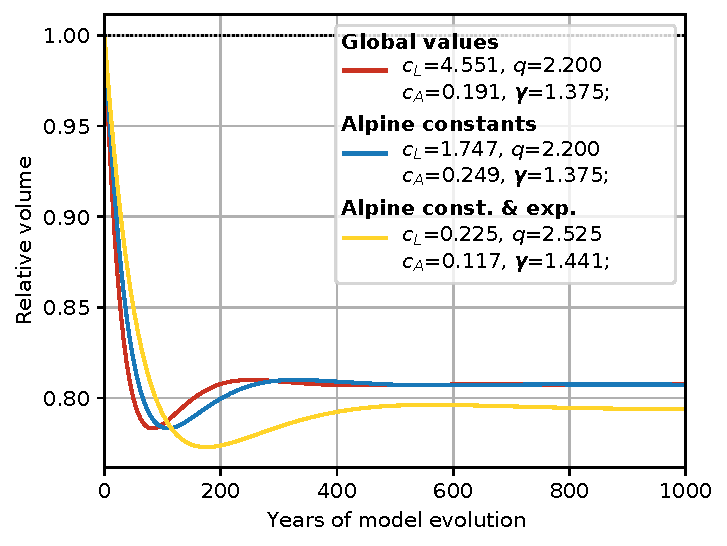
\includegraphics[width=\textwidth]{../plots/final_plots/sensitivity/scaling_params_histalp.pdf}
      \end{subfigure}
      
      \caption{Temporal evolution of glacier ice volume under a positive temperature bias of \SI{+0.5}{\celsius} for the Hintereisferner (RGI60-11.00897) in the two upper panels (\subref{fig:sensitivity:time_scales_hef}) and (\subref{fig:sensitivity:scaling_params_hef}) and for the entire HISTALP domain in the two lower panels (\subref{fig:sensitivity:time_scales_histalp}) and (\subref{fig:sensitivity:scaling_params_histalp}). The right panels show results for different model-internal time scales, scaled by a linear factor (see legend for details). The left panels show results for different scaling constants and scaling exponents (see legend for details). Note the difference in y-axis scales.}
      \label{fig:sensitivity}
    \end{figure}

    \subsection{Sensitivity to model-internal time scales} % (fold)
    \label{sec:sensitivity_to_model_internal_time_scales_results}
      Let's again start with the Hintereisferner test case, before moving to the regional scale. As was to be expected, the model-internal time scales do not affect the absolute values, but control only the oscillatory behavior. The e-folding response time scales for length and area are directly proportional to the model-internal time scales. Halving and doubling the time scales results in a respective change of \SI{-4}{\year} and \SI{+7}{\year} for the area response time and \SI{-10}{\year} and \SI{+15}{\year} for the length response time\footnote{The changes refer to the values shown in Section~\ref{sec:single_glacier_test_case_results}.}. The asymmetric responses hint at the non-linear effect of the time scales. Interestingly enough, the e-folding response time for volume is indirectly proportional to the model internal time scales, and changes only by \SI{\pm1}{\year}. This means, while the glacier takes longer to reach it's new equilibrium area and length, it takes less time to reach the new equilibrium volume (and vice versa). This is, however, most likely just a mathematical artifact, which stems from the oscillatory behavior and is discussed in the following.

      The main change, however, is seen in the oscillation amplitude (Figure~\ref{fig:sensitivity:time_scales_hef}). The damping ratio seems to be controlled by the model-internal time scales. Higher model-internal time scales lead to stronger oscillations and vice versa. But even with halved model-internal time scales, the modeled volume adjustment still shows some oscillations. With the default values, the \vas{} model overshoots the volume change estimate by \SI{5}{\percent} of the final equilibrium value and it takes 371 years to reach an equilibrium. Hereby, an equilibrium state is (somewhat arbitrarily) defined as the range of \SI{\pm0.1}{\percent} of the equilibrium value at year 1000. Halving and doubling the model-internal time scales changes the overshoot to \SI{1}{\percent} and \SI{11}{\percent} of the equilibrium value, respectively. The time span until a new equilibrium is reached seems to be almost linearly dependent on the model-internal time scales. By halving and doubling the model-internal time scales it takes 150 years and 688 years for the model to reach a new steady state, respectively.

      The same qualitative findings are made for the regional run with all Alpiner glaciers (Figure~\ref{fig:sensitivity:time_scales_histalp}). The absolute values do not change for different model-internal time scales, only the oscillatory behavior does. While longer model-internal time scales result again in stronger overshoots, the oscillations seem generally more damped for the regional run. This is most likely a side effect of the summation over all Alpine glacier, whereby small scale oscillations can cancel each other out. The overshoots amount to \SI{0.2}{\percent}, \SI{3.0}{\percent} and \SI{8.0}{\percent} of the equilibrium value for a time scale factor of 0.5, 1 and 2, respectively. Thereby it takes 133 years, 335 years and 642 years to reach a new steady state. When halving the model-internal time scales, the aggregate volume evolution shows almost no more discernible oscillations and is basically of exponential (asymptotic) nature.

    % subsection sensitivity_to_model_internal_time_scales_results (end)

    \subsection{Sensitivity to scaling parameters} % (fold)
    \label{sec:sensitivity_to_scaling_parameters_results}

      As seen above, the model-internal time scale do not change the absolute values of any geometric glacier property. So what about the scaling parameters?! The following paragraph compares the model behavior between the custom Hintereisferner scaling constants and the global scaling constants (Figure\ref{fig:sensitivity:scaling_params_hef}). The scaling exponents are held constant, since it is not possible to compute a linear regression from a single data point (see Section~\ref{sub:sensitivity_experiments_setup} for details). % $c_L = \SI{1.555}{\meter^{3-q}}$ and $c_A = \SI{0.252}{\meter^{3-2\gamma}}$ and the global scaling constants $c_L = \SI{4.551}{\meter^{3-q}}$ and $c_A = \SI{0.191}{\meter^{3-2\gamma}}$.
      Changing the scaling constants leads to different absolute values. As explained in Section~\ref{sub:glacier_evolution_model_implementation}, the \vas{} model starts by computing the initial glacier volume from the surface area via the \vas{} relation. Hence, the initial area stays the same while the initial ice volume increases with the custom scaling constants. The initial volume for the Hintereisferner increases to \SI{0.787}{\cubic\kilo\meter} with custom scaling constants $c_L = \SI{1.555}{\meter^{3-q}}$ and $c_A = \SI{0.252}{\meter^{3-2\gamma}}$, compared to the \SI{0.596}{\cubic\kilo\meter} with the global values. While starting with a larger initial ice volume increases the absolute change in ice volume (\SI{-0.120}{\cubic\kilo\meter} vs. \SI{-0.091}{\cubic\kilo\meter}), it still results in a larger equilibrium ice volume (\SI{0.667}{\cubic\kilo\meter} vs. \SI{0.506}{\cubic\kilo\meter}). However, when normalized with the respective initial ice volumes, the changes in ice volume, the equilibrium values and the overshoots (i.e., minimum values due to the oscillatory behavior) are almost identical (the differences lie far below \SI{0.1}{\percent}). This comes as no surprise, since the scaling constants are canceled out during the normalization process. In fact, when estimating \emph{changes} in regional or global ice volume the scaling constant $c$ can be eliminated altogether \citep[][Section 8.5]{Bahr2015}. While the relative values do not change, the temporal evolution does. As already discussed, the bigger custom scaling constant $c_A$ leads to a bigger initial ice volume. Increasing the glacier's ice volume in turn increases the glacier's response time, since larger glaciers generally react slower to climatic changes. The volume e-folding response time increases to 30 years with the custom scaling constants, compared to 23 years with the global values. The increased response time goes hand in hand with a stronger oscillation. While the amplitude stays the same, the frequency decreases. Hence, the peak of the overshoot shifts by 28 years (to year 100 after the initial climate perturbation) and it takes much longer to reach the new equilibrium state (493 years vs. 371 years).
      While the glacier length reacts analogously to the custom scaling constants, the surface area does not. This was to be expected, since the initial surface area does not depend on the scaling parameters. While the equilibrium value and the e-folding response time are practically not affected, the oscillation amplifies. In addition to the decreased frequency, as for ice volume and glacier length, the surface area overshoots by \SI{15\,761}{\square\meter} more under the custom scaling constants (which corresponds to \SI{\approx0.2}{\percent} of the equilibrium value).
      
      Again, the results of regional Alpine run (Figure\ref{fig:sensitivity:scaling_params_histalp}) are analogous to the Hintereisferner test case. While the Hintereisferner test case compares only the global and custom scaling constants, an additional run with custom scaling constants and scaling exponents is investigated (see Section~\ref{sub:sensitivity_experiments_setup} for details). As seen above, changing the scaling constants results in different absolute values (for the initial volume as well as for the final equilibrium volume). However, when normalized with the initial values only the run with custom scaling exponents shows a different (bigger) change in ice volume. The total modeled glacier ice volume shrinks from an initial \SI{229.7}{\cubic\kilo\meter} to a final \SI{182.4}{\cubic\kilo\meter}, subjected to a positive temperature bias of \SI{+0.5}{\celsius}. The change of \SI{-47.3}{\cubic\kilo\meter} corresponds to \SI{-21}{\percent} of the initial value. However, the result does still not compare to the \SI{-47}{\percent} of the flowline model and is not even significantly different from the \SI{-19}{\percent} for the other two \vas{} runs.

    % subsection sensitivity_to_scaling_parameters_results (end)


  % section sensitivity_experiments_results (end)

  \section{Commitment runs} % (fold)
  \label{sec:commitment_runs_results}

    The easiest way of projecting future glacier mass change is by so called commitment experiments. While an accurate projection should be forced by GCM ensemble data, based on different emission scenarios, a simpler approach will suffice for this qualitative comparison of the \vas{} and flowline model. Thereby, different possible warming scenarios can be simulated by committing to todays climate and adding different positive temperature biases. For details about the experimental setup see Section~\ref{sub:commitment_runs_setup}. Figure~\ref{fig:histalp_commitment} shows the evolution of relative and absolute ice volume of all Alpine glaciers under different warming scenarios.

    Before starting with the results, a disclaimer is in order. As can be seen in the sections above, the \vas{} has some flaws when compared to the flowline model. However, since no validation against observational data was performed, no statement about the accuracy of the model accuracy can be made here. All that said, the following section should be seen as the culmination of all the work done above. And while the results may not hold up or even be entirely meaningless compared to recently published projections, they can serve as reference point on what to expect from a flowline model compared to the \vas{} model.

    Again, all characteristic established for the \vas{} model can be seen here as well: initial ice volume and ice volume changes are underestimated; the new equilibrium values are reached faster; the ice volume estimations overshoot and rebound; the symmetric behavior can not be asses since only positive temperature perturbations are used. Expressed in numbers: the \vas{} model estimates an ice volume change of \SI{42}{\cubic\kilo\meter} and \SI{88}{\cubic\kilo\meter} from an initial \SI{130}{\cubic\kilo\meter} to a final \SI{88}{\cubic\kilo\meter} and \SI{42}{\cubic\kilo\meter} for todays climate with \SI{0}{\celsius} and \SI{+2}{\celsius}, respectively. This corresponds to a relative loss in ice volume of \SI{-68}{\percent} under the \SI{+2}{\celsius} warming scenario. The flowline model already estimates a relative ice loss \SI{-66}{\percent} for todays climate without any temperature bias. And after one-hundred years under the \SI{+2}{\celsius} warming scenario, only \SI{8}{\percent} of glacier ice are left. These differences are even more drastic in absolute numbers, since the flowline starts with \SI{34}{\cubic\kilo\meter} more total ice volume. This suggests that ice change projections made with scaling models are most likely lower bound estimates.

    \begin{figure}[htp]
      \centering
      \begin{subfigure}[b]{0.48\textwidth}
        \caption{\Vas{} model, relative glacier volume}
        \label{fig:histalp_projection:volume_norm_const}
        \centering
        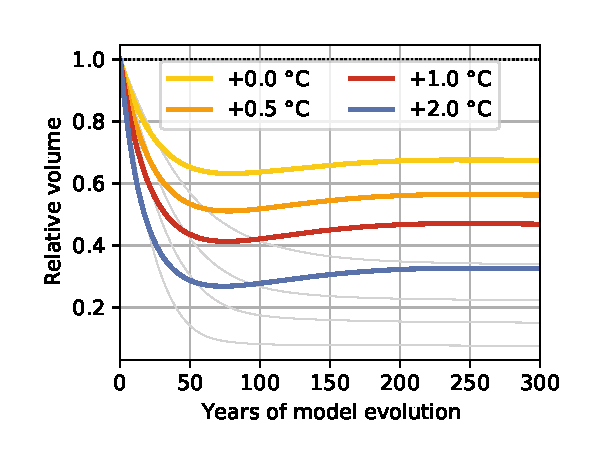
\includegraphics[width=\textwidth]{../plots/final_plots/time_series/histalp_projection/volume_norm_vas.pdf}
      \end{subfigure}
      \hfill
      \begin{subfigure}[b]{0.48\textwidth}
        \caption{Flowline model, relative glacier volume}
        \label{fig:histalp_projection:volume_norm_random}
        \centering
        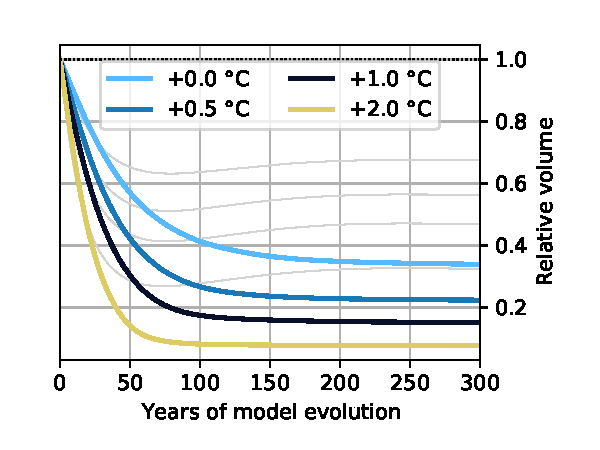
\includegraphics[width=\textwidth]{../plots/final_plots/time_series/histalp_projection/volume_norm_fl.pdf}
      \end{subfigure}
      \begin{subfigure}[b]{0.48\textwidth}
        \caption{\Vas{} model, absolute glacier volume}
        \label{fig:histalp_projection:volume_abs_const}
        \centering
        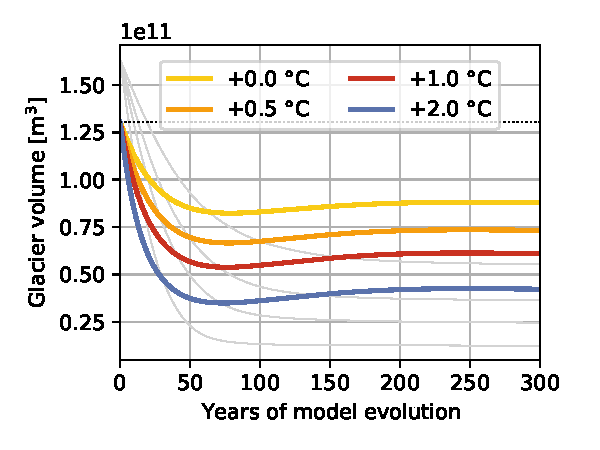
\includegraphics[width=\textwidth]{../plots/final_plots/time_series/histalp_projection/volume_abs_vas.pdf}
      \end{subfigure}
      \hfill
      \begin{subfigure}[b]{0.48\textwidth}
        \caption{Flowline model, absolute glacier volume}
        \label{fig:histalp_projection:volume_abs_random}
        \centering
        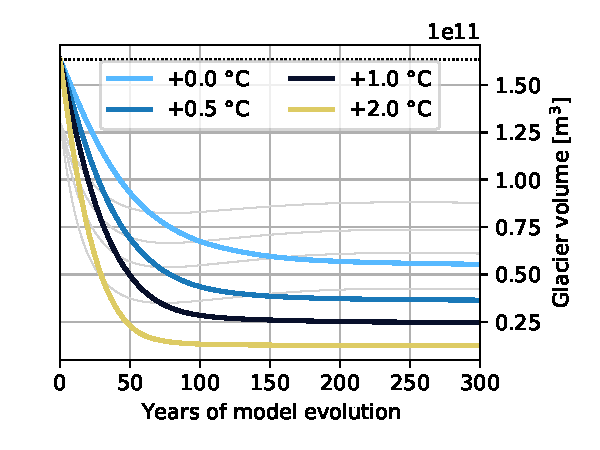
\includegraphics[width=\textwidth]{../plots/final_plots/time_series/histalp_projection/volume_abs_fl.pdf}
      \end{subfigure}
      
      \caption{Time series of total ice volume for all glaciers in the HISTALP domain. The upper two panels show the relative glacier ice volume, normalized with the initial values, while the lower two panels show the absolute glacier ice volume. The left panels show the result of the \vas{} model, the right panels show the results of the flowline model. Solid lines represent the random climate scenarios, while dashed lines represent the constant climate scenarios. All climate scenarios are based on an equilibrium climate, with one of three different temperature biases.
      Yellow, orange and red solid lines represent the \vas{} model, while cyan, blue and purple solid lines represent the flowline model, under a random climate with a temperature bias of \SI{-.5}{\celsius}, \SI{0}{\celsius} and \SI{+.5}{\celsius}, respectively. Yellow, orange and red dashed lines represent the \vas{} model, while cyan, blue and purple dashed lines represent the flowline model, under a constant climate with a temperature bias of \SI{-.5}{\celsius}, \SI{0}{\celsius} and \SI{+.5}{\celsius}, respectively. %TODO change colors
      The dotted line indicate the initial volume. The light gray lines represent the volume evolutions of the other model, to facilitate comparisons.}
      \label{fig:histalp_projection}
    \end{figure}


  % section commitment_runs_results (end)

% section future_projection (end)





\newpage
\thispagestyle{plain}


% ==== DISCUSSION ==============================================================
% ---- set some counters to zero:
\setcounter{equation}{0}
\setcounter{table}{0}
\setcounter{figure}{0}
% ---- include tex-file:
%!TEX root = thesis.tex
\chapter{Discussion}\label{chap:discussion}
\thispagestyle{plain}

% The discussion is the interpretation and evaluation of the results. It is a
% comparison of your results with previous findings. It provides the answer to
% the scientific questions raised in the introduction. It is the "nerve center"
% of a thesis, whereas the chapter Results may be seen as the "heart".

% Clearly separate between your own contributions and those of others. Provide
% rigorous citations of appropriate sources! Explicitly refer to specific 
% results presented earlier. A certain amount of repetition is necessary. Order
% discussion items not chronologically but rather logically.

% The chapter Results answers the question: What has been found? (Facts). The
% chapter Discussion answers the question: How has the  result to be interpreted?
% (Opinion).

% The most important message should appear in the first paragraph. The answer to
% the key question may appear in the first sentence: e.g., did your original idea
% work, or didn't it? The following questions may be answered in the discussion
% section:
% - Why is the presented method simpler, better, more reliable than previous
% ones?
% - What are its strengths and its limitations?
% - How significant are the results?
% - How trustworthy are the observations?
% - Under which conditions and for which region are the results/method valid?
% - Can the results be easily transferred to other regions or fields?


\newpage
\thispagestyle{plain}


% ==== CONCLUSIONS =============================================================
% ---- set some counters to zero:
\setcounter{equation}{0}
\setcounter{table}{0}
\setcounter{figure}{0}
% ---- include tex-file:
%!TEX root = thesis.tex
\chapter{Conclusions}\label{chap:conclusions}
\thispagestyle{plain}

% This chapter contains consequences that derive from your results. It may also
% contain speculations. It may provide suggestions for future studies. Hence,
% the conclusions may provide an outlook and list open questions. Sometimes this
% chapter is part of the discussion. In such a case, the chapter reads
% "Discussion and Conclusions".

Glaciers are controlled by their mass balance and the resulting ice flow. Hence, a glacier model has to incorporate a mass balance model, to account for accumulation and ablation, and a dynamic model, to update glacier geometries in response to mass balance changes. A dynamic model based on scaling relations, such as the here presented combination of volume/area, volume/length and response time scaling, can produce qualitatively comparable results to a state-of-the-art flowline model. Thereby, the results of real world applications like projections of regional glacial evolution forced by GCM models are mostly within the uncertainty bounds of each other, while idealized equilibrium experiments expose the limitations and shortcommings of the \vas{} model.

The overall behavior of the \vas{} model is as expected, i.e., the model correctly simulates advances and retreats in response to step changes in climate as well as to natural climate variability, it has the ability to reach a new equilibrium, and it shows characteristics of a low-pass filter. However, changes in ice volume, surface area and glacier length are generally underestimated when compared to the flowline model. The model-internal representation of time scales has been identified as the main source of those differences and other unexpected and unwanted behaviors. The conducted sensitivity analysis, backed by \citet{Roe2020}, concludes that the used time scale parameterization results in too high values. The timescales could be exploited as future tuning parameter. Using the geometric timescales based on the terminus ablation rate \citep{Johannesson1989} rather than the turnover may improve the results.

Additional errors are introduced by missing physically relevant processes, which are not resolved by the \vas{} model. Those include but are not limited to, a missing mass-balance-elevation feedback, a constant average slope, and no awareness of the surrounding topography. While these processes may be secondary on a global scale, estimates for regions with many small glaciers like the Alps vary significantely between scaling and flowline model. The usage of more complex models is advisable for future projections of glacier mass changes, especially given the nowadays available computational power.

This study detailed the underlying principles and implementation process of a simple global glacier model based on glacier scaling relations \citep{Marzeion2012b} in the OGGM framework. The implementation of the \vas{} model in the OGGM framework is a success on its own. As suggested by \citet{Maussion2019}, the implementation of simpler approaches, such as the one presented here, allows to test the benefits of the increased model complexity. Such extension of the OGGM are obviously not limited to simple model, but may as well add more complex processes \citep[e.g., an improved calving parametrization,][]{Recinos2019}. It shows the benefits of an open source, modular, community driven glacier model. Comparing different parametrization and estimating uncertainties are imperative to improve projections of future glacier mass loss and its consequences. The global implementation of the scaling model and the implementation of additional geometry parameterizations \citep[e.g., GloGEM by][]{Huss2015} could give further insights into the benefits and limitations of explicit glacier dynamics.

\newpage
\thispagestyle{plain}


% ==== APPENDIX ================================================================
% ---- start appendix:
\appendix
% ---- set some counters to zero:
\setcounter{equation}{0}
\setcounter{table}{0}
\setcounter{figure}{0}
% ---- include tex-file:
%!TEX root = thesis.tex

% Singel glacier test cases
\chapter{Single glacier test cases}\label{appendix_A}
\thispagestyle{plain}

The first experiment was performed as a single glacier test case on the example of Hintereisferner (RGI60-11.00897), see Section~\ref{sub:experimental_setup_test_case} for details on the experimental setup. The test case was intended to get a first qualitative impression, drawing conclusions from a single data point is, however, still questionable. Therefore, the exact same experiment was performed on five more single glaciers (Pasterze, Mer de Glace, Glacier d'Argentière, Großer Aletschgletscher, Rhonegletscher) and the results are shown here below. While there are differences between the different glaciers, all general findings presented in Section~\ref{sub:results_test_case} hold true.

\begin{figure}[p]
  \centering

  % VAS volume
  \begin{subfigure}[b]{0.476\textwidth}
    \caption{\Vas{} model, relative ice volume}
    \label{fig:Pasterze:volume_vas}
    \centering
    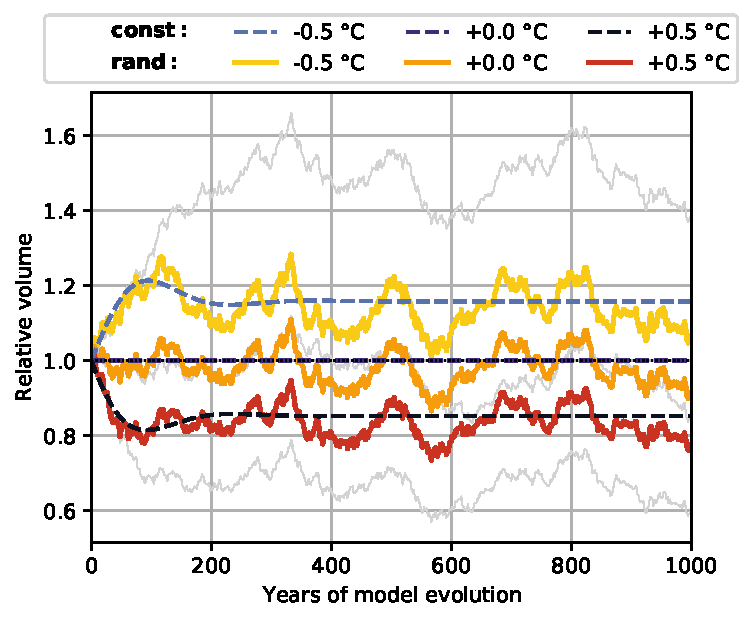
\includegraphics[width=\textwidth]{../plots/final_plots/time_series/single_glaciers/volume_norm_vas_Pasterze.pdf}
  \end{subfigure}
  \hfill
  % Flowline volume
  \begin{subfigure}[b]{0.476\textwidth}
    \caption{Flowline model, relative ice volume}
    \label{fig:Pasterze:volume_fl}
    \centering
    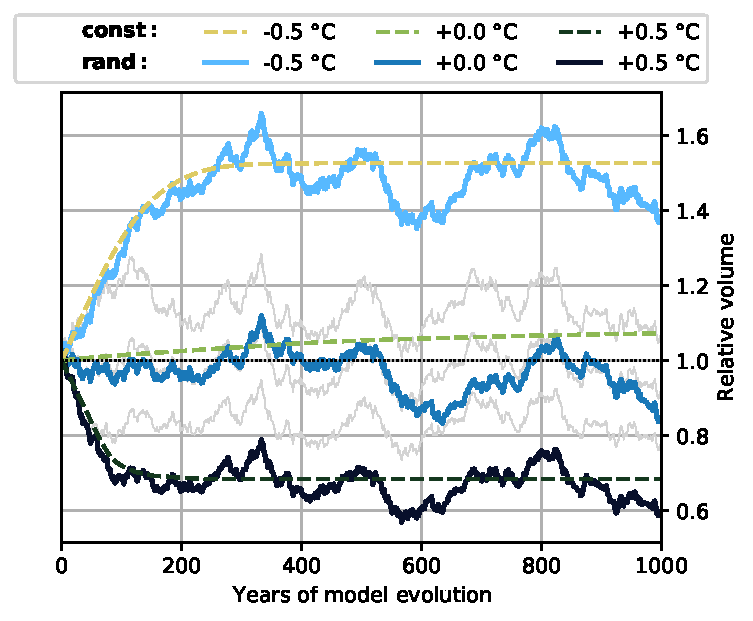
\includegraphics[width=\textwidth]{../plots/final_plots/time_series/single_glaciers/volume_norm_fl_Pasterze.pdf}
  \end{subfigure}

  % VAS area
  \begin{subfigure}[b]{0.476\textwidth}
    \caption{\Vas{} model, relative surface area}
    \label{fig:Pasterze:area_vas}
    \centering
    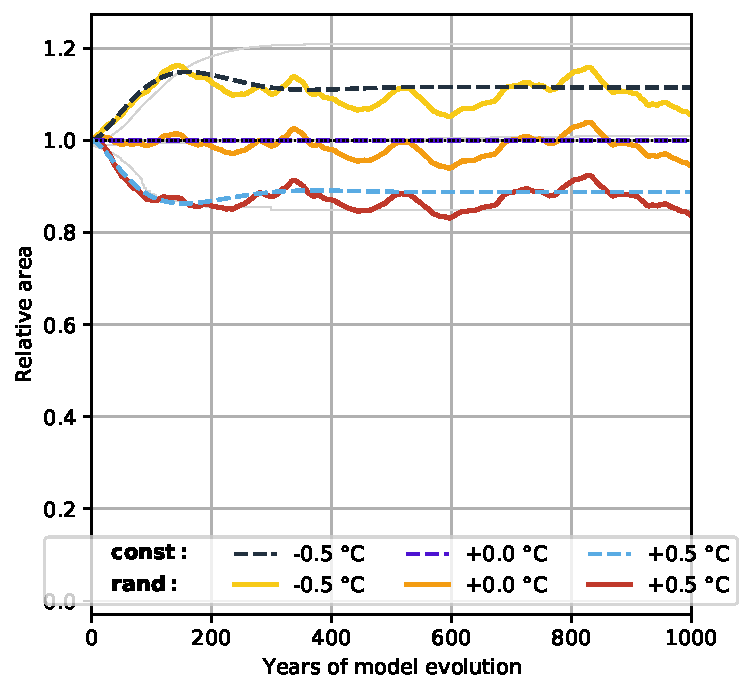
\includegraphics[width=\textwidth]{../plots/final_plots/time_series/single_glaciers/area_norm_vas_Pasterze.pdf}
  \end{subfigure}
  \hfill
  % Flowline area
  \begin{subfigure}[b]{0.476\textwidth}
    \caption{Flowline model, relative surface area}
    \label{fig:Pasterze:area_fl}
    \centering
    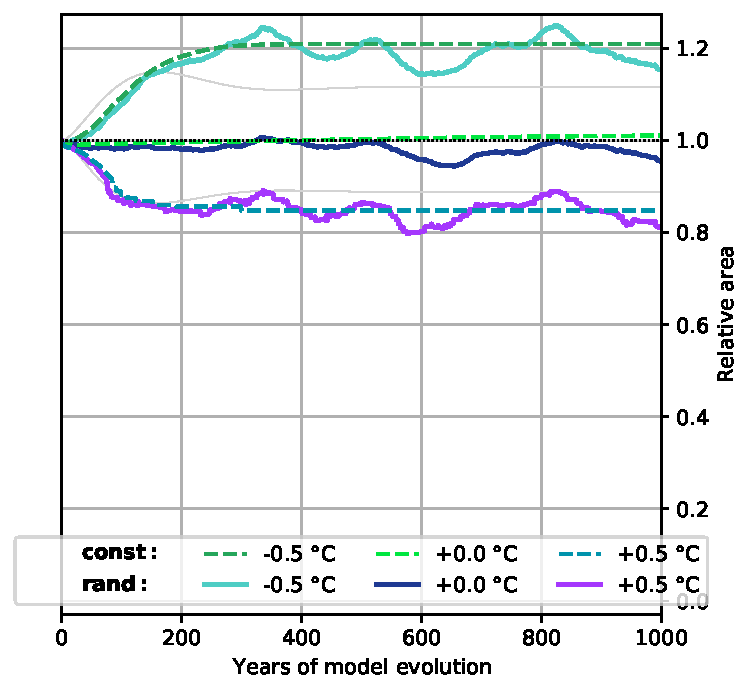
\includegraphics[width=\textwidth]{../plots/final_plots/time_series/single_glaciers/area_norm_fl_Pasterze.pdf}
  \end{subfigure}

  % VAS length
  \begin{subfigure}[b]{0.476\textwidth}
    \caption{\Vas{} model, relative glacier length}
    \label{fig:Pasterze:length_vas}
    \centering
    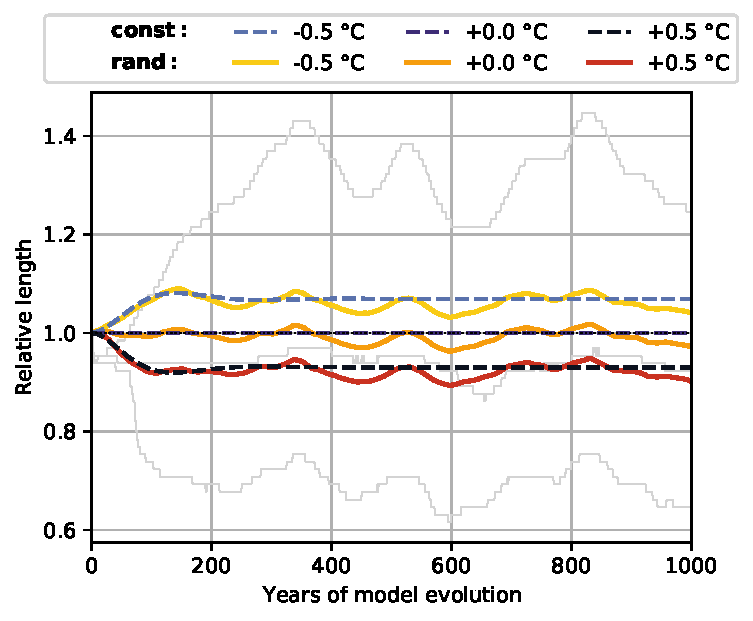
\includegraphics[width=\textwidth]{../plots/final_plots/time_series/single_glaciers/length_norm_vas_Pasterze.pdf}
  \end{subfigure}
  \hfill
  % Flowline length
  \begin{subfigure}[b]{0.476\textwidth}
    \caption{Flowline model, relative glacier length}
    \label{fig:Pasterze:length_fl}
    \centering
    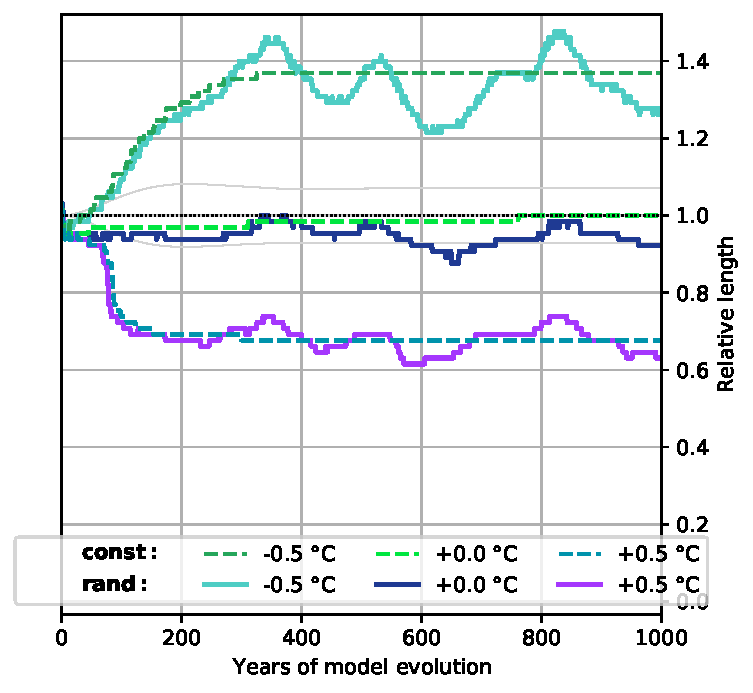
\includegraphics[width=\textwidth]{../plots/final_plots/time_series/single_glaciers/length_norm_fl_Pasterze.pdf}
  \end{subfigure}
  
  \caption{Temporal evolution of ice volume in (\subref{fig:Pasterze:volume_vas}) and (\subref{fig:Pasterze:volume_fl}), surface area in (\subref{fig:Pasterze:area_vas}) and (\subref{fig:Pasterze:area_fl}) and glacier length in (\subref{fig:Pasterze:length_vas}) and (\subref{fig:Pasterze:length_fl}) for \textbf{Pasterze (RGI60-11.00106)}. The shown values area normalized with their respective initial values. The left panels show the result of the \vas{} model, the right panels show the results of the flowline model. Solid lines represent the random climate scenarios, while dashed lines represent the constant climate scenarios. All climate scenarios are based on an equilibrium climate. The applied temperature biases of \SI{-.5}{\celsius}, \SI{0}{\celsius} and \SI{+.5}{\celsius} are color coded, see legend for details. The dotted line indicates the initial volume. The light gray lines represent the volume evolutions of the other model, to facilitate comparisons.}
  \label{fig:Pasterze}
\end{figure}

\begin{figure}[p]
  \centering

  % VAS volume
  \begin{subfigure}[b]{0.476\textwidth}
    \caption{\Vas{} model, relative ice volume}
    \label{fig:Mer_de_Glace:volume_vas}
    \centering
    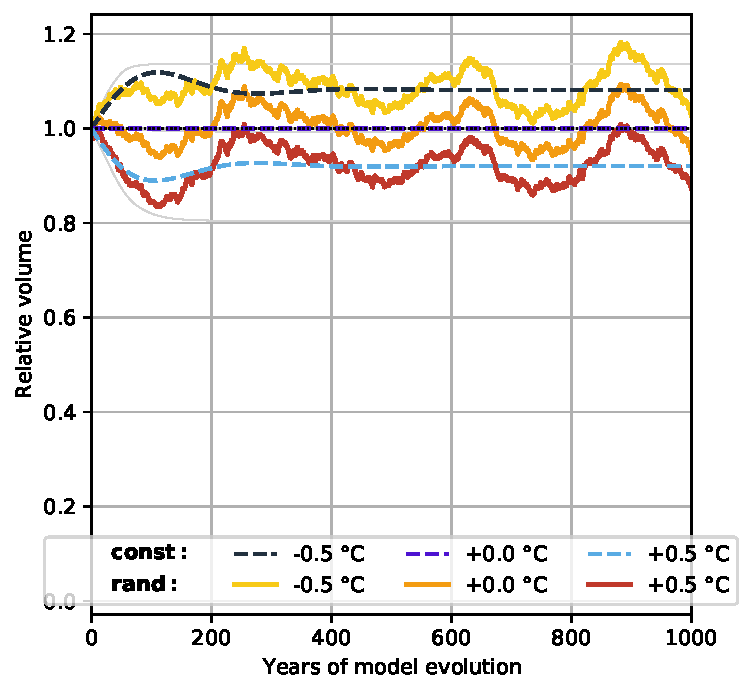
\includegraphics[width=\textwidth]{../plots/final_plots/time_series/single_glaciers/volume_norm_vas_Mer_de_Glace.pdf}
  \end{subfigure}
  \hfill
  % Flowline volume
  \begin{subfigure}[b]{0.476\textwidth}
    \caption{Flowline model, relative ice volume}
    \label{fig:Mer_de_Glace:volume_fl}
    \centering
    \includegraphics[width=\textwidth]{../plots/final_plots/time_series/single_glaciers/volume_norm_fl_Mer_de_Glace.pdf}
  \end{subfigure}

  % VAS area
  \begin{subfigure}[b]{0.476\textwidth}
    \caption{\Vas{} model, relative surface area}
    \label{fig:Mer_de_Glace:area_vas}
    \centering
    \includegraphics[width=\textwidth]{../plots/final_plots/time_series/single_glaciers/area_norm_vas_Mer_de_Glace.pdf}
  \end{subfigure}
  \hfill
  % Flowline area
  \begin{subfigure}[b]{0.476\textwidth}
    \caption{Flowline model, relative surface area}
    \label{fig:Mer_de_Glace:area_fl}
    \centering
    \includegraphics[width=\textwidth]{../plots/final_plots/time_series/single_glaciers/area_norm_fl_Mer_de_Glace.pdf}
  \end{subfigure}

  % VAS length
  \begin{subfigure}[b]{0.476\textwidth}
    \caption{\Vas{} model, relative glacier length}
    \label{fig:Mer_de_Glace:length_vas}
    \centering
    \includegraphics[width=\textwidth]{../plots/final_plots/time_series/single_glaciers/length_norm_vas_Mer_de_Glace.pdf}
  \end{subfigure}
  \hfill
  % Flowline length
  \begin{subfigure}[b]{0.476\textwidth}
    \caption{Flowline model, relative glacier length}
    \label{fig:Mer_de_Glace:length_fl}
    \centering
    \includegraphics[width=\textwidth]{../plots/final_plots/time_series/single_glaciers/length_norm_fl_Mer_de_Glace.pdf}
  \end{subfigure}
  
  \caption{Temporal evolution of ice volume in (\subref{fig:Mer_de_Glace:volume_vas}) and (\subref{fig:Mer_de_Glace:volume_fl}), surface area in (\subref{fig:Mer_de_Glace:area_vas}) and (\subref{fig:Mer_de_Glace:area_fl}) and glacier length in (\subref{fig:Mer_de_Glace:length_vas}) and (\subref{fig:Mer_de_Glace:length_fl}) for \textbf{Mer de Glace (RGI60-11.03643)}. The shown values area normalized with their respective initial values. The left panels show the result of the \vas{} model, the right panels show the results of the flowline model. Solid lines represent the random climate scenarios, while dashed lines represent the constant climate scenarios. All climate scenarios are based on an equilibrium climate. The applied temperature biases of \SI{-.5}{\celsius}, \SI{0}{\celsius} and \SI{+.5}{\celsius} are color coded, see legend for details. The dotted line indicates the initial volume. The light gray lines represent the volume evolutions of the other model, to facilitate comparisons.}
  \label{fig:Mer_de_Glace}
\end{figure}

\begin{figure}[p]
  \centering

  % VAS volume
  \begin{subfigure}[b]{0.476\textwidth}
    \caption{\Vas{} model, relative ice volume}
    \label{fig:Glacier_d_Argentiere:volume_vas}
    \centering
    \includegraphics[width=\textwidth]{../plots/final_plots/time_series/single_glaciers/volume_norm_vas_Glacier_d'Argentière.pdf}
  \end{subfigure}
  \hfill
  % Flowline volume
  \begin{subfigure}[b]{0.476\textwidth}
    \caption{Flowline model, relative ice volume}
    \label{fig:Glacier_d_Argentiere:volume_fl}
    \centering
    \includegraphics[width=\textwidth]{../plots/final_plots/time_series/single_glaciers/volume_norm_fl_Glacier_d'Argentière.pdf}
  \end{subfigure}

  % VAS area
  \begin{subfigure}[b]{0.476\textwidth}
    \caption{\Vas{} model, relative surface area}
    \label{fig:Glacier_d_Argentiere:area_vas}
    \centering
    \includegraphics[width=\textwidth]{../plots/final_plots/time_series/single_glaciers/area_norm_vas_Glacier_d'Argentière.pdf}
  \end{subfigure}
  \hfill
  % Flowline area
  \begin{subfigure}[b]{0.476\textwidth}
    \caption{Flowline model, relative surface area}
    \label{fig:Glacier_d_Argentiere:area_fl}
    \centering
    \includegraphics[width=\textwidth]{../plots/final_plots/time_series/single_glaciers/area_norm_fl_Glacier_d'Argentière.pdf}
  \end{subfigure}

  % VAS length
  \begin{subfigure}[b]{0.476\textwidth}
    \caption{\Vas{} model, relative glacier length}
    \label{fig:Glacier_d_Argentiere:length_vas}
    \centering
    \includegraphics[width=\textwidth]{../plots/final_plots/time_series/single_glaciers/length_norm_vas_Glacier_d'Argentière.pdf}
  \end{subfigure}
  \hfill
  % Flowline length
  \begin{subfigure}[b]{0.476\textwidth}
    \caption{Flowline model, relative glacier length}
    \label{fig:Glacier_d_Argentiere:length_fl}
    \centering
    \includegraphics[width=\textwidth]{../plots/final_plots/time_series/single_glaciers/length_norm_fl_Glacier_d'Argentière.pdf}
  \end{subfigure}
  
  \caption{Temporal evolution of ice volume in (\subref{fig:Glacier_d_Argentiere:volume_vas}) and (\subref{fig:Glacier_d_Argentiere:volume_fl}), surface area in (\subref{fig:Glacier_d_Argentiere:area_vas}) and (\subref{fig:Glacier_d_Argentiere:area_fl}) and glacier length in (\subref{fig:Glacier_d_Argentiere:length_vas}) and (\subref{fig:Glacier_d_Argentiere:length_fl}) for \textbf{Glacier d'Argentière (RGI60-11.03638)}. The shown values area normalized with their respective initial values. The left panels show the result of the \vas{} model, the right panels show the results of the flowline model. Solid lines represent the random climate scenarios, while dashed lines represent the constant climate scenarios. All climate scenarios are based on an equilibrium climate. The applied temperature biases of \SI{-.5}{\celsius}, \SI{0}{\celsius} and \SI{+.5}{\celsius} are color coded, see legend for details. The dotted line indicates the initial volume. The light gray lines represent the volume evolutions of the other model, to facilitate comparisons.}
  \label{fig:Glacier_d_Argentiere}
\end{figure}

\begin{figure}[p]
  \centering

  % VAS volume
  \begin{subfigure}[b]{0.476\textwidth}
    \caption{\Vas{} model, relative ice volume}
    \label{fig:Grosser_Aletschgletscher:volume_vas}
    \centering
    \includegraphics[width=\textwidth]{../plots/final_plots/time_series/single_glaciers/volume_norm_vas_Großer_Aletschgletscher.pdf}
  \end{subfigure}
  \hfill
  % Flowline volume
  \begin{subfigure}[b]{0.476\textwidth}
    \caption{Flowline model, relative ice volume}
    \label{fig:Grosser_Aletschgletscher:volume_fl}
    \centering
    \includegraphics[width=\textwidth]{../plots/final_plots/time_series/single_glaciers/volume_norm_fl_Großer_Aletschgletscher.pdf}
  \end{subfigure}

  % VAS area
  \begin{subfigure}[b]{0.476\textwidth}
    \caption{\Vas{} model, relative surface area}
    \label{fig:Grosser_Aletschgletscher:area_vas}
    \centering
    \includegraphics[width=\textwidth]{../plots/final_plots/time_series/single_glaciers/area_norm_vas_Großer_Aletschgletscher.pdf}
  \end{subfigure}
  \hfill
  % Flowline area
  \begin{subfigure}[b]{0.476\textwidth}
    \caption{Flowline model, relative surface area}
    \label{fig:Grosser_Aletschgletscher:area_fl}
    \centering
    \includegraphics[width=\textwidth]{../plots/final_plots/time_series/single_glaciers/area_norm_fl_Großer_Aletschgletscher.pdf}
  \end{subfigure}

  % VAS length
  \begin{subfigure}[b]{0.476\textwidth}
    \caption{\Vas{} model, relative glacier length}
    \label{fig:Grosser_Aletschgletscher:length_vas}
    \centering
    \includegraphics[width=\textwidth]{../plots/final_plots/time_series/single_glaciers/length_norm_vas_Großer_Aletschgletscher.pdf}
  \end{subfigure}
  \hfill
  % Flowline length
  \begin{subfigure}[b]{0.476\textwidth}
    \caption{Flowline model, relative glacier length}
    \label{fig:Grosser_Aletschgletscher:length_fl}
    \centering
    \includegraphics[width=\textwidth]{../plots/final_plots/time_series/single_glaciers/length_norm_fl_Großer_Aletschgletscher.pdf}
  \end{subfigure}
  
  \caption{Temporal evolution of ice volume in (\subref{fig:Grosser_Aletschgletscher:volume_vas}) and (\subref{fig:Grosser_Aletschgletscher:volume_fl}), surface area in (\subref{fig:Grosser_Aletschgletscher:area_vas}) and (\subref{fig:Grosser_Aletschgletscher:area_fl}) and glacier length in (\subref{fig:Grosser_Aletschgletscher:length_vas}) and (\subref{fig:Grosser_Aletschgletscher:length_fl}) for \textbf{Großer Aletschgletscher (RGI60-11.01450)}. The shown values area normalized with their respective initial values. The left panels show the result of the \vas{} model, the right panels show the results of the flowline model. Solid lines represent the random climate scenarios, while dashed lines represent the constant climate scenarios. All climate scenarios are based on an equilibrium climate. The applied temperature biases of \SI{-.5}{\celsius}, \SI{0}{\celsius} and \SI{+.5}{\celsius} are color coded, see legend for details. The dotted line indicates the initial volume. The light gray lines represent the volume evolutions of the other model, to facilitate comparisons.}
  \label{fig:Grosser_Aletschgletscher}
\end{figure}

\begin{figure}[p]
  \centering

  % VAS volume
  \begin{subfigure}[b]{0.476\textwidth}
    \caption{\Vas{} model, relative ice volume}
    \label{fig:Rhonegletscher:volume_vas}
    \centering
    \includegraphics[width=\textwidth]{../plots/final_plots/time_series/single_glaciers/volume_norm_vas_Rhonegletscher.pdf}
  \end{subfigure}
  \hfill
  % Flowline volume
  \begin{subfigure}[b]{0.476\textwidth}
    \caption{Flowline model, relative ice volume}
    \label{fig:Rhonegletscher:volume_fl}
    \centering
    \includegraphics[width=\textwidth]{../plots/final_plots/time_series/single_glaciers/volume_norm_fl_Rhonegletscher.pdf}
  \end{subfigure}

  % VAS area
  \begin{subfigure}[b]{0.476\textwidth}
    \caption{\Vas{} model, relative surface area}
    \label{fig:Rhonegletscher:area_vas}
    \centering
    \includegraphics[width=\textwidth]{../plots/final_plots/time_series/single_glaciers/area_norm_vas_Rhonegletscher.pdf}
  \end{subfigure}
  \hfill
  % Flowline area
  \begin{subfigure}[b]{0.476\textwidth}
    \caption{Flowline model, relative surface area}
    \label{fig:Rhonegletscher:area_fl}
    \centering
    \includegraphics[width=\textwidth]{../plots/final_plots/time_series/single_glaciers/area_norm_fl_Rhonegletscher.pdf}
  \end{subfigure}

  % VAS length
  \begin{subfigure}[b]{0.476\textwidth}
    \caption{\Vas{} model, relative glacier length}
    \label{fig:Rhonegletscher:length_vas}
    \centering
    \includegraphics[width=\textwidth]{../plots/final_plots/time_series/single_glaciers/length_norm_vas_Rhonegletscher.pdf}
  \end{subfigure}
  \hfill
  % Flowline length
  \begin{subfigure}[b]{0.476\textwidth}
    \caption{Flowline model, relative glacier length}
    \label{fig:Rhonegletscher:length_fl}
    \centering
    \includegraphics[width=\textwidth]{../plots/final_plots/time_series/single_glaciers/length_norm_fl_Rhonegletscher.pdf}
  \end{subfigure}
  
  \caption{Temporal evolution of ice volume in (\subref{fig:Rhonegletscher:volume_vas}) and (\subref{fig:Rhonegletscher:volume_fl}), surface area in (\subref{fig:Rhonegletscher:area_vas}) and (\subref{fig:Rhonegletscher:area_fl}) and glacier length in (\subref{fig:Rhonegletscher:length_vas}) and (\subref{fig:Rhonegletscher:length_fl}) for \textbf{Rhonegletscher (RGI60-11.01238)}. The shown values area normalized with their respective initial values. The left panels show the result of the \vas{} model, the right panels show the results of the flowline model. Solid lines represent the random climate scenarios, while dashed lines represent the constant climate scenarios. All climate scenarios are based on an equilibrium climate. The applied temperature biases of \SI{-.5}{\celsius}, \SI{0}{\celsius} and \SI{+.5}{\celsius} are color coded, see legend for details. The dotted line indicates the initial volume. The light gray lines represent the volume evolutions of the other model, to facilitate comparisons.}
  \label{fig:Rhonegletscher}
\end{figure}

\chapter{ARMA model order}\label{appendix_B}
\thispagestyle{plain}

\begin{figure}[h!]
  \centering

  % AR
  \begin{subfigure}[b]{0.5\textwidth}
    \caption{Order $p$ for the autoregressive term}
    \label{fig:arma:arp}
    \centering
    \includegraphics[width=\textwidth]{../plots/final_plots/arma/arp.pdf}
  \end{subfigure}
  \hfill
  % MA
  \begin{subfigure}[b]{0.5\textwidth}
    \caption{Order $q$ for the moving-average term}
    \label{fig:arma:maq}
    \centering
    \includegraphics[width=\textwidth]{../plots/final_plots/arma/maq.pdf}
  \end{subfigure}
  
  \caption{Orders $p$ and $q$ for a potential ARMA($p$,$q$) model, estimated from the ACFs and PACFs of the length change signal in response to a white noise climate (see Section~\ref{sub:autocorrelation_function_results})}.
  \label{fig:arma}
\end{figure}


\newpage
\thispagestyle{plain}


% ==== START BACK MATTER (this has no visual effect)============================
\backmatter 


% ==== BIBLIOGRAPHY ============================================================
\addcontentsline{toc}{chapter}{Bibliography}
% ---- use AMS reference format (use file ametsoc.bst included in ...
%      ... http://www.ametsoc.org/pubs/journals/AMS_Latex_V3.0.tar.gz):s
\bibliographystyle{./ametsoc}   % ametsoc.bst in local directory
% ---- use BibTeX database file:
\bibliography{./master}
\newpage
\thispagestyle{plain}


% ==== ACKNOWLEDGMENTS =========================================================
% ---- include tex-file:
%!TEX root = thesis.tex
\chapter*{Acknowledgments}
\addcontentsline{toc}{chapter}{Acknowledgments}
\thispagestyle{plain}
\noindent First and foremost I want to thank my supervisor Fabien Maussion. He sparked the idea of implementing the \vas{} model during the Hacktoberfest 2018 at our institute; he gave me the liberty and the time I needed to develop and test ideas, make my own mistakes and learn from them while still providing guidance and tutelage; and most importantly, over the last couple of months he steered me towards the finish line and was an essential help in sharpening my points and in finalizing this entire project.\\[0.3cm]
\noindent Additional thanks go to Ben Marzeion for providing me with the original model code and answering some questions about the implementation and conceptual details, as well as Matthias Dusch, Jan-Hendrik Malles, Timo Rothenspieler and the entire OGGM community for helping with coding problems and providing feedback to model results.\\[0.3cm]
\noindent I would like to thank my parents and grandparents for their continued support, not only during my studies but throughout my life. Special thanks go to my fiancée Carmen for her encouragement and moral support, and also just for enduring me during the more stressful times.\\[0.3cm]
\noindent Furthermore I would like to thank everybody else not mentioned by name who contributed to this thesis in any way, shape or form: by engaging in thematic discussions about harmonic oscillations or color schemes, by calling or swinging by and providing some much needed distraction, or by motivating me when I was about to throw it all away.\\[0.3cm]
\noindent And ``last but not least'', to quote Snoop Dogg, ``I want to thank me. I want to thank me for believing in me. I want to thank me for doing all this hard work. [...] I want to thank me for never quitting.''
\newpage
\thispagestyle{plain}


% ==== CURRICULUM VITAE ========================================================
% ---- include tex-file:
%!TEX root = thesis.tex
\chapter*{Curriculum Vitae}
\addcontentsline{toc}{chapter}{Curriculum Vitae}
\thispagestyle{plain}
%
%
% ---- name, address, and date of birth:
\vspace{-0.5cm}
FirstName LastName\\
Address\\
Born on 01 April 1976 in Town, Country
\\[5mm]
%
%
% ---- education:
\textsc{Education and Professional training}:
\\[1ex]
\begin{tabular}{@{} p{2.5cm} @{} p{12.5cm} @{}}
1999--2003 &
Research assistant and Ph.D. student in the group of Dr. LastName at the
Institute of Meteorology and Geophysics, University of Innsbruck. \\[1ex]
1998--1999 &
Diploma thesis under the guidance of Dr. LastName,
Institute of Meteorology and Geophysics, University of Innsbruck:
\textit{``Title of your diploma thesis''}. \\[1ex]
1993--1998 &
Diploma study at the University of Innsbruck.
\textit{Master of Natural Science (Magister rerum naturalium)} in Meteorology.
\\[1ex]
1989--1993 &
Highschool, Town. \textit{Matura}.
\end{tabular}
\\[5mm]
%
%
% ---- training courses:
\textsc{Meteorological training courses}:
``Numerical methods and adiabatic formulation of models'', ECMWF, 1998; ``Data
assimilation and use of satellite data'', ECMWF, 1998.
\\[5mm]
%
%
% ---- field experiments:
\textsc{Participation in field experiments}:
Gap flow study (MAP), Austria, 1999.

\newpage
\thispagestyle{plain}


% ==== EPILOGUE ================================================================
% ---- include tex-file:
%!TEX root = thesis.tex
\chapter*{Epilogue}
\addcontentsline{toc}{chapter}{Epilogue}
\thispagestyle{plain}

Here is the place where you may want to tell a little story or a fairy tale
which has some relevance for your thesis, such as ``Once upon a time, \dots''.
The Epilogue is optional.

\newpage
\thispagestyle{plain}


\end{document}
% ==== END OF BODY =============================================================
